\newcommand{\suppsection}[1]{\section{{\fontsize{12}{13}\selectfont #1}}}

\renewcommand{\tmpwidth}{18mm}
\setlength{\tabcolsep}{1pt}


\twocolumn[
\begin{@twocolumnfalse}
{
\begin{center}
\begin{tabular}{m{20mm}m{2mm} cccc c cccc}

Original & 
&
&&& \parbox[c]{\tmpwidth}{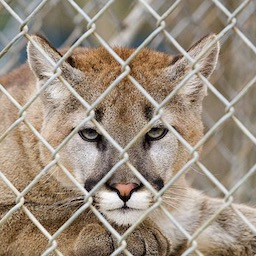
\includegraphics[width=\tmpwidth]{figures/analysis/cougar.jpeg}} &
&
&&& \parbox[c]{\tmpwidth}{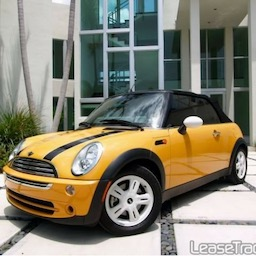
\includegraphics[width=\tmpwidth]{figures/analysis/car.jpeg}} 
\\
\\[-4pt]
&
& Mask 95\% & Mask 90\% & Mask 85\% & Mask 75\% &
& Mask 95\% & Mask 90\% & Mask 85\% & Mask 75\% 
\\ 
\parbox[l]{15mm}{\small{Example Input Mask}} &
&
\parbox[c]{\tmpwidth}{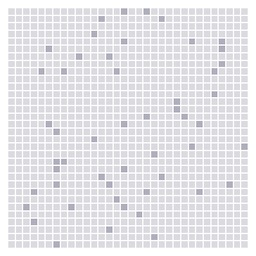
\includegraphics[width=\tmpwidth]{figures/analysis/000286_39_mask03_95.jpeg}}&
\parbox[c]{\tmpwidth}{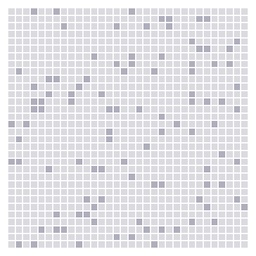
\includegraphics[width=\tmpwidth]{figures/analysis/000286_0_mask01_90.jpeg}}&
\parbox[c]{\tmpwidth}{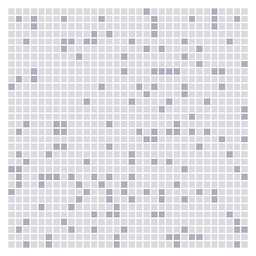
\includegraphics[width=\tmpwidth]{figures/analysis/000286_2_mask_01_85.jpeg}}&
\parbox[c]{\tmpwidth}{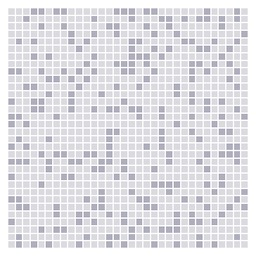
\includegraphics[width=\tmpwidth]{figures/analysis/000286_0_mask03_75.jpeg}}&
&
\parbox[c]{\tmpwidth}{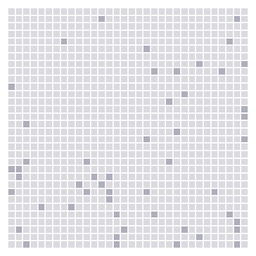
\includegraphics[width=\tmpwidth]{figures/analysis/000511_2_mask_95.jpeg}}&
\parbox[c]{\tmpwidth}{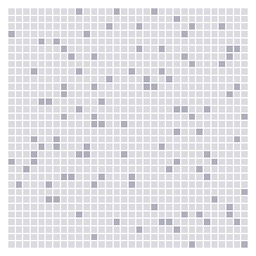
\includegraphics[width=\tmpwidth]{figures/analysis/000511_0_mask_90.jpeg}}&
\parbox[c]{\tmpwidth}{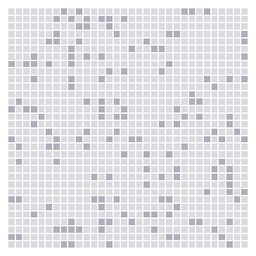
\includegraphics[width=\tmpwidth]{figures/analysis/000511_5_mask_85.jpeg}}&
\parbox[c]{\tmpwidth}{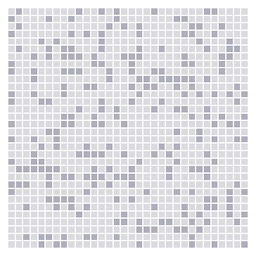
\includegraphics[width=\tmpwidth]{figures/analysis/000511_0_mask_75.jpeg}}

\\
\parbox[l]{15mm}{\small{Reconstruction Sample}} &
&
\parbox[c]{\tmpwidth}{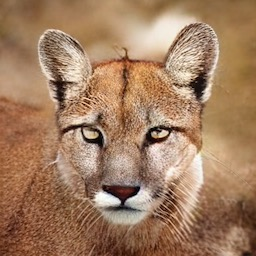
\includegraphics[width=\tmpwidth]{figures/analysis/000286_39_output_95.jpeg}}&
\parbox[c]{\tmpwidth}{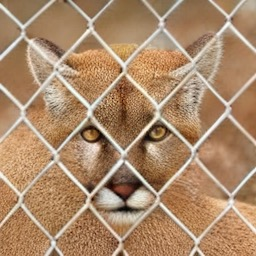
\includegraphics[width=\tmpwidth]{figures/analysis/000286_0_output_90.jpeg}}&
\parbox[c]{\tmpwidth}{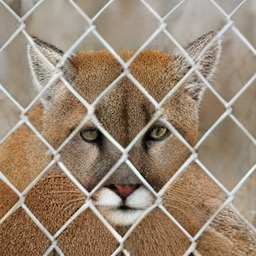
\includegraphics[width=\tmpwidth]{figures/analysis/cougar_85.jpeg}}&
\parbox[c]{\tmpwidth}{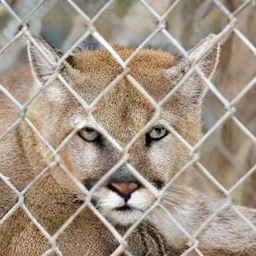
\includegraphics[width=\tmpwidth]{figures/analysis/cougar_75.jpeg}}&
&
\parbox[c]{\tmpwidth}{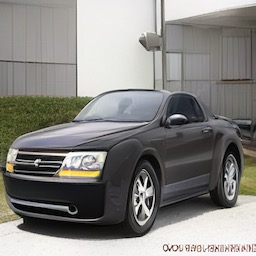
\includegraphics[width=\tmpwidth]{figures/analysis/car_95.jpeg}}&
\parbox[c]{\tmpwidth}{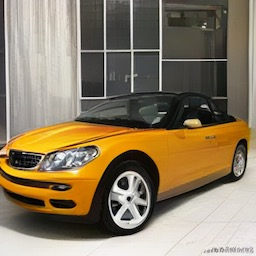
\includegraphics[width=\tmpwidth]{figures/analysis/car_90.jpeg}}&
\parbox[c]{\tmpwidth}{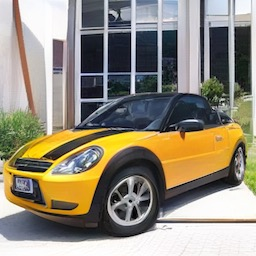
\includegraphics[width=\tmpwidth]{figures/analysis/car_85.jpeg}}&
\parbox[c]{\tmpwidth}{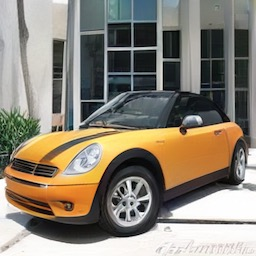
\includegraphics[width=\tmpwidth]{figures/analysis/car_75.jpeg}}

\\
\parbox[l]{20mm}{\small{Median of $100$ Samples}}
 & 
&
\parbox[c]{\tmpwidth}{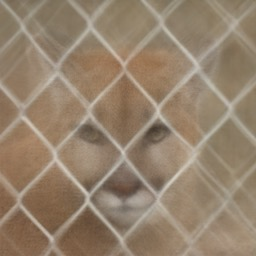
\includegraphics[width=\tmpwidth]{figures/analysis/why_schedule_cougar_statistics_95percent_avg.jpeg}}&
\parbox[c]{\tmpwidth}{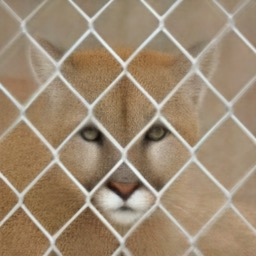
\includegraphics[width=\tmpwidth]{figures/analysis/why_schedule_cougar_statistics_90percent_median.jpeg}}&
\parbox[c]{\tmpwidth}{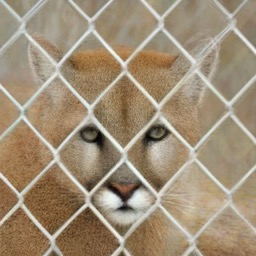
\includegraphics[width=\tmpwidth]{figures/analysis/why_schedule_cougar_85percent_median.jpeg}}&
\parbox[c]{\tmpwidth}{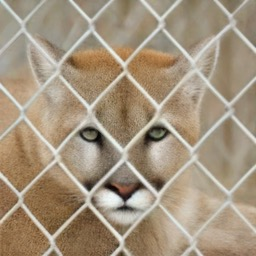
\includegraphics[width=\tmpwidth]{figures/analysis/why_schedule_cougar_statistics_75percent_median.jpeg}}&
&
\parbox[c]{\tmpwidth}{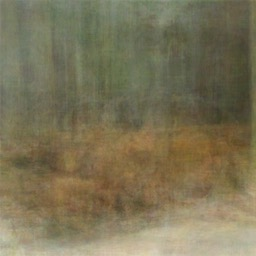
\includegraphics[width=\tmpwidth]{figures/analysis/why_schedule_car_statistics_95percent_median.jpeg}}&
\parbox[c]{\tmpwidth}{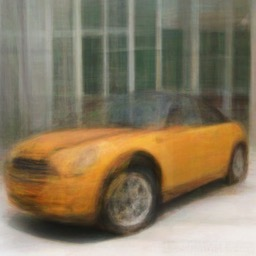
\includegraphics[width=\tmpwidth]{figures/analysis/why_schedule_car_statistics_90percent_median.jpeg}}&
\parbox[c]{\tmpwidth}{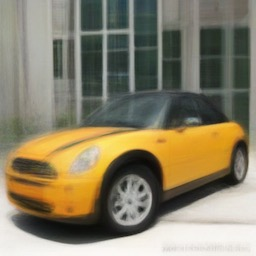
\includegraphics[width=\tmpwidth]{figures/analysis/why_schedule_car_statistics_85percent_median.jpeg}}&
\parbox[c]{\tmpwidth}{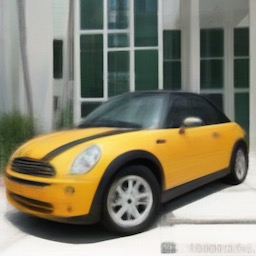
\includegraphics[width=\tmpwidth]{figures/analysis/why_schedule_car_statistics1_75percent_median.jpeg}}
\\
\end{tabular}
\captionof{figure}{\textbf{Examples of \model on Image Reconstruction.} \model takes in masked tokens extracted from original images (row one) using random input masks (row two, with unknown tokens marked in light gray), and outputs reconstructed images (row three). We then randomly sample 100 masks with the same mask ratio, and illustrate the median of the 100 reconstructed samples in row four.}
% The sharpness of the median may be interpreted as the consensus among the reconstruction samples.}
\label{fig:supp_reconstruction}
\end{center}
\vspace{10mm}
}
\end{@twocolumnfalse}
]

\suppsection{Discussion on Image Reconstruction}
\label{sec:supp_reconstruction_discussion}

In \ref{ssec:class_conditional_synthesis}, we primarily evaluate \model on class-conditional image generation tasks. Here we offer more discussion on its performance on image reconstruction. We set up by first randomly sampling input mask $M$ with a mask ratio $r$ of the visual tokens masked out, and then running \model's iterative decoding algorithm to reconstruct images. Figure~\ref{fig:analysis_psnr} shows the PSNR and LPIPS\cite{zhang2018lpips} of the reconstructed samples as functions of $r$, whereas Figure~\ref{fig:supp_reconstruction} visualizes two examples of this process with $r$ ranging from $95\%$ to $75\%$. 


We observe that \model reconstructs holistic information (\eg pose and shape of the foreground objects) even with a very high percentage (\eg 95\%) of tokens masked out. More importantly, there seems to exist an inflection point around 90\%: while both reconstruction quality and consistency improve drastically as the mask ratio decreases until 90\%, after 90\% further improvements are slowed down. This observation is corroborated by the large jump in the visual similarity between reconstruction samples and the original images from 95\% to 90\% in Figure~\ref{fig:supp_reconstruction}, \eg the fence in front of the tiger and the car's color are consistently captured once the mask ratio is below 90\%, but not at 95\%.

In other words, we find that visual tokens are highly redundant. For a holistic reconstruction, only a very small portion (\eg 10\%) of the tokens are essential; the remaining ones merely improve the recovery of finer appearance or details. This echos our intuition behind the masking design laid out in \ref{ssec:masking} that the prediction of the first few tokens is key to image generation. Similar observations on the spatial redundancy of images are discussed in a concurrent paper MAE~\cite{he2021mae}. In their work, they find that masking a high proportion of the input image yields a nontrivial and meaningful self-supervisory task for image representation learning.

\setlength{\tabcolsep}{2pt}

\begin{figure}[!h]
    \centering
    \begin{tabular}{cc}
     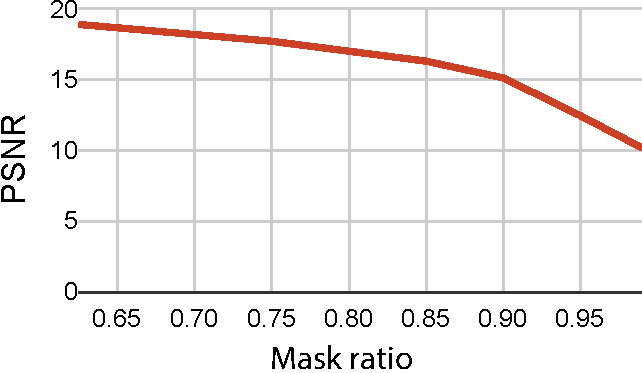
\includegraphics[width=41mm]{figures/analysis/psnr_single2.pdf} & 
      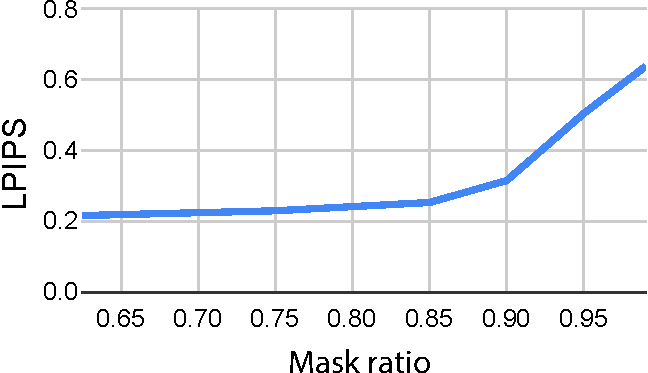
\includegraphics[width=41mm]{figures/analysis/lpips_single2.pdf} 
    \end{tabular}
      \vspace{-3mm}
    \caption{通过 PSNR 和 LPIPS\cite{zhang2018lpips} 衡量的重建质量和多样性。}
    \label{fig:analysis_psnr}
    \vspace{-3mm}
\end{figure}

\suppsection{Additional Class-conditional Image Generation Results}
\label{sec:supp_diversity_comparison}
 
In this section, we report additional results on class-conditional image generation.

We follow prior transformer-based methods\cite{Razavi19vqvae2,Esser21vqgan} to employ the classifier-based rejection sampling to improve the sample quality scores. Specifically, we use a pre-trained ResNet classifier\cite{ResNet} to score output samples based on the predicted probability and keep samples with an acceptance rate of $0.05$, as in VQGAN~\cite{Esser21vqgan}. 
As shown in Table \ref{tab:supp_cc_classifier}, MaskGIT demonstrates consistent improvement over VQGAN, and is comparable with ADM with classifier guidance~\cite{dhariwal2021diffusion}. More importantly, by adding the rejection sampling, \model achieves state-of-the-art Inception Scores ($355.6$ on 256$\times$256 and $342.0$ on 512$\times$512). 



In Table~\ref{tab:supp_cas}, we report Precision and Recall scores calculated using Inception features~\cite{christian16inception}. In contrast to the VGG\cite{simonyan2015vgg} feature-based scores, which we report in Table~\ref{tab:maintable} for a more direct comparison with prior work~\cite{KynkaanniemiKLL19,dhariwal2021diffusion}, we find that the Inception feature-based scores are more consistent with our qualitative observations that VQGAN’s samples are more diverse than BigGAN’s. Under both measures, \model’s recall scores outperform those of BigGAN and VQGAN. We also report CAS evaluated on classifiers trained without augmentation from RandAugment\cite{cubuk2019randaugment}. Consistent with our main results, \model outperforms BigGAN and our baseline VQGAN by a large margin.

Finally, we show a few comparisons of the class-conditional samples generated by \model with the samples generated by BigGAN-deep and VQVAE-2 in Figure~\ref{fig:supp_cc_diversity}, \ref{fig:supp_cc_diversity_1}, and \ref{fig:supp_cc_diversity_2}.


\setlength{\tabcolsep}{4pt}
\begin{table}[ht]
\small
    \centering
    
    \resizebox{0.97\linewidth}{!}{
        \begin{tabular}{lc l lc cc}
        \toprule
Dataset && Model & Classifier guidance && FID & IS          \\ 
\midrule
% ADM~[9]  & & & 23.24& 58.06 && 10.94 & 101.0  \\
% % VQ-GAN~[11]       & & & n/a & n/a && 15.78 & 78.3  \\
% VQGAN\cite{Esser21vqgan} & & & 26.52$^\ast$ & 66.18$^\ast$ && 15.78 & 78.3 \\
% MaskGIT                         & & & 7.32 & 156.0 && 6.18 & 182.1 \\ \cline{2-8}

ImageNet && ADM~\cite{dhariwal2021diffusion}  & 1.0 guidance  && 4.59 & 186.70 \\
256$\times$256 && VQGAN~\cite{Esser21vqgan} & 0.05 acceptance rate    &&  5.88 & 304.8 \\
&& MaskGIT & 0.05 acceptance rate    &          & \textbf{4.02} & \textbf{355.6} \\ \midrule
ImageNet && ADM~\cite{dhariwal2021diffusion}  & 1.0 guidance  && 7.72 & 172.71 \\
% 512x512 && VQGAN~\cite{Esser21vqgan}$^\ast$ & 0.05 acceptance rate && &  \\
512$\times$512 && MaskGIT & 0.05 acceptance rate    && \textbf{4.46} & \textbf{342.0} \\
  \bottomrule
    \end{tabular}
    
    }
    \vspace{-1mm}
    \caption{\small{ImageNet 上带有分类器引导的方法的类条件图像合成。
    %\small{$^\ast$ denotes the model we train with the same architecture and setup with ours.}
    }}
    \label{tab:supp_cc_classifier}
\vspace{-5mm}
\end{table}

\newcolumntype{N}{@{}m{0pt}@{}}
\setlength{\tabcolsep}{2.5pt}
\begin{table}[!th]
\small
    \centering
    \resizebox{.93\linewidth}{!}{
    \begin{tabular}{lc ccc ccc }
    \toprule
     {Model} & 
     &  {Prec}  $\uparrow$ & {Rec}   $\uparrow$ &
     & \multicolumn{2}{c}{{{CAS} $\times 100$} $\uparrow$}  
     \\
     \cline{6-7}
    & &&& &{{Top-1 (73.1)}} & {{Top-5 (91.5)}} \\
   % \textbf{ImageNet 256$\times$256}  &&& &&& &
   %\\[-2pt]
    \midrule
     
    BigGAN-deep~\cite{biggan}  & %, 1.0 trunc. &
    & \textbf{0.82} & 0.27 &
    & 42.65 &65.92 
    \\
    VQ-GAN$^\ast$ &
    & 0.61 & 0.47 &
    & 47.50 & 68.90
    \\
    \bfseries{\model (Ours)} &
    & 0.78 & \bfseries{0.50} &
   & \bfseries{58.20} & \bfseries{79.65} 

    \\
    % \textbf{ImageNet 512$\times$512} &&& &&& &\\[-2pt]
    % \midrule
    
    %  BigGAN-deep~\cite{biggan} & 
    %  & \textbf{0.88} & 0.29 &
    %  &44.02&68.22
    %  \\
    %  VQGAN$^\ast$ &
    %  & 0.73 & 0.31 &
    %   &51.29&74.24 \\
      
    %  \bfseries{\model (Ours)} & 
    %  &  0.78 & 0.50 &
    %  &63.43&84.79 \\
    %  % \bfseries{Ours}, 0.5 RS & ? & ? & &  \\
    \bottomrule
    
    \end{tabular}
    }
    \vspace{-1mm}
    \caption{在ImageNet 256$\times$256上与BigGAN-deep和我们的基线VQGAN的更多定量比较。
    \footnotesize{$^\ast$表示我们用与我们相同的架构和设置训练的模型。}
    }
    \vspace{-5mm}
    \label{tab:supp_cas}
    % On average 10-15ms per step

\end{table}
\renewcommand{\tmpwidth}{50mm}
\setlength{\tabcolsep}{2pt}
\begin{figure*}[!ht]
    \centering
    \begin{tabular}{c c c}

   
    BigGAN-deep (FID=$6.95$) & VQVAE-2$^\dagger$ (FID=$31$) & \model  (FID=\bestfid) \\
    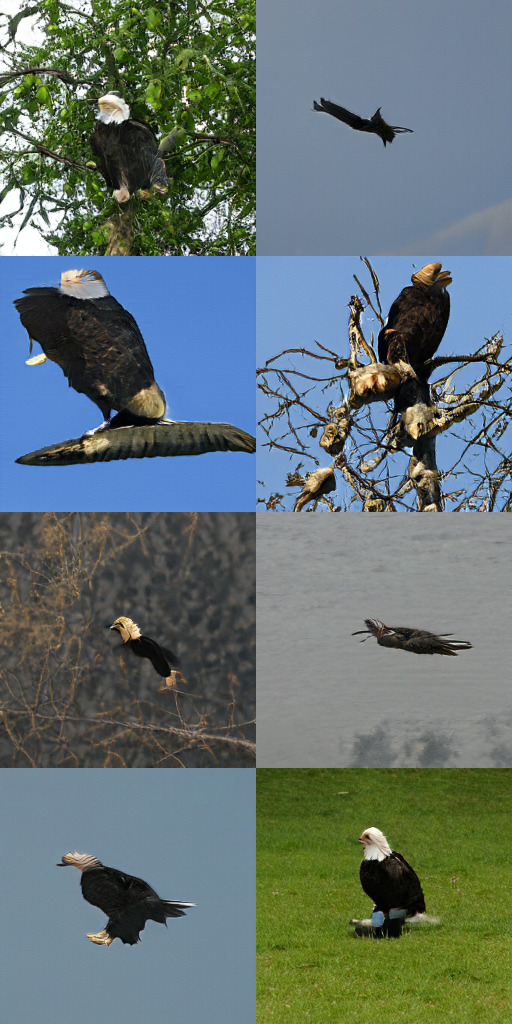
\includegraphics[ width=\tmpwidth]{figures/supp_cc/22_bald-eagle_biggan.jpg} & 
    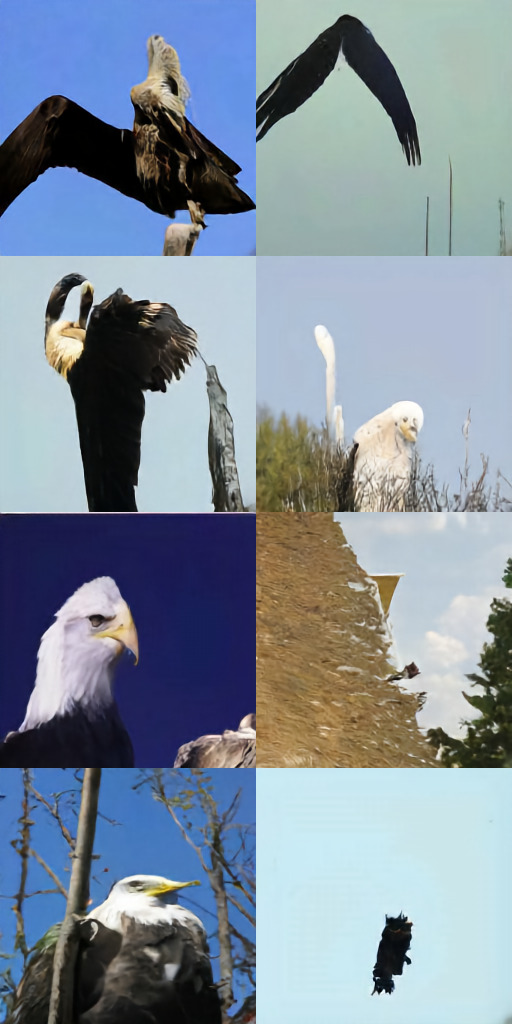
\includegraphics[ width=\tmpwidth]{figures/supp_cc/22_bald-eagle_vqvae2.jpg}& 
    % 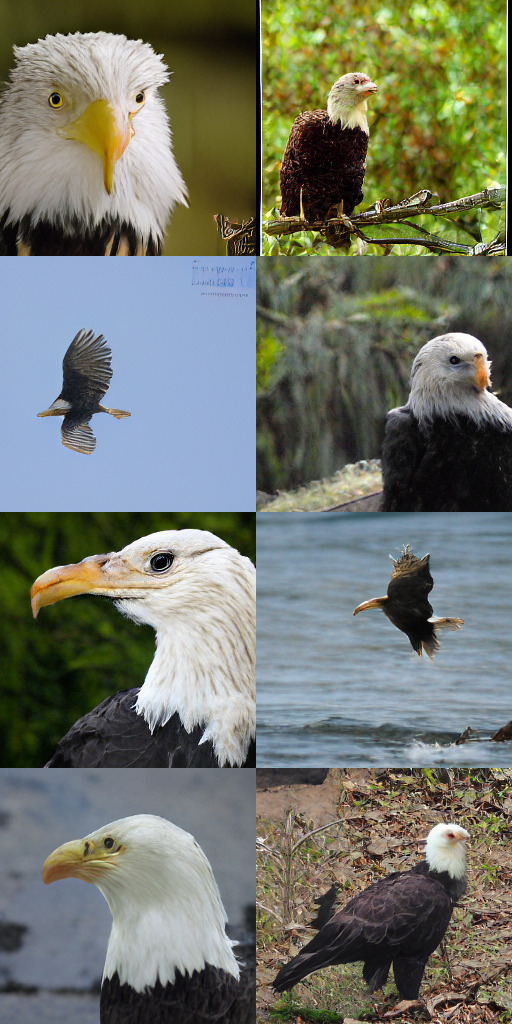
\includegraphics[ width=\tmpwidth]{figures/supp_cc/22_bald-eagle_vqgan.jpg} & \ 
    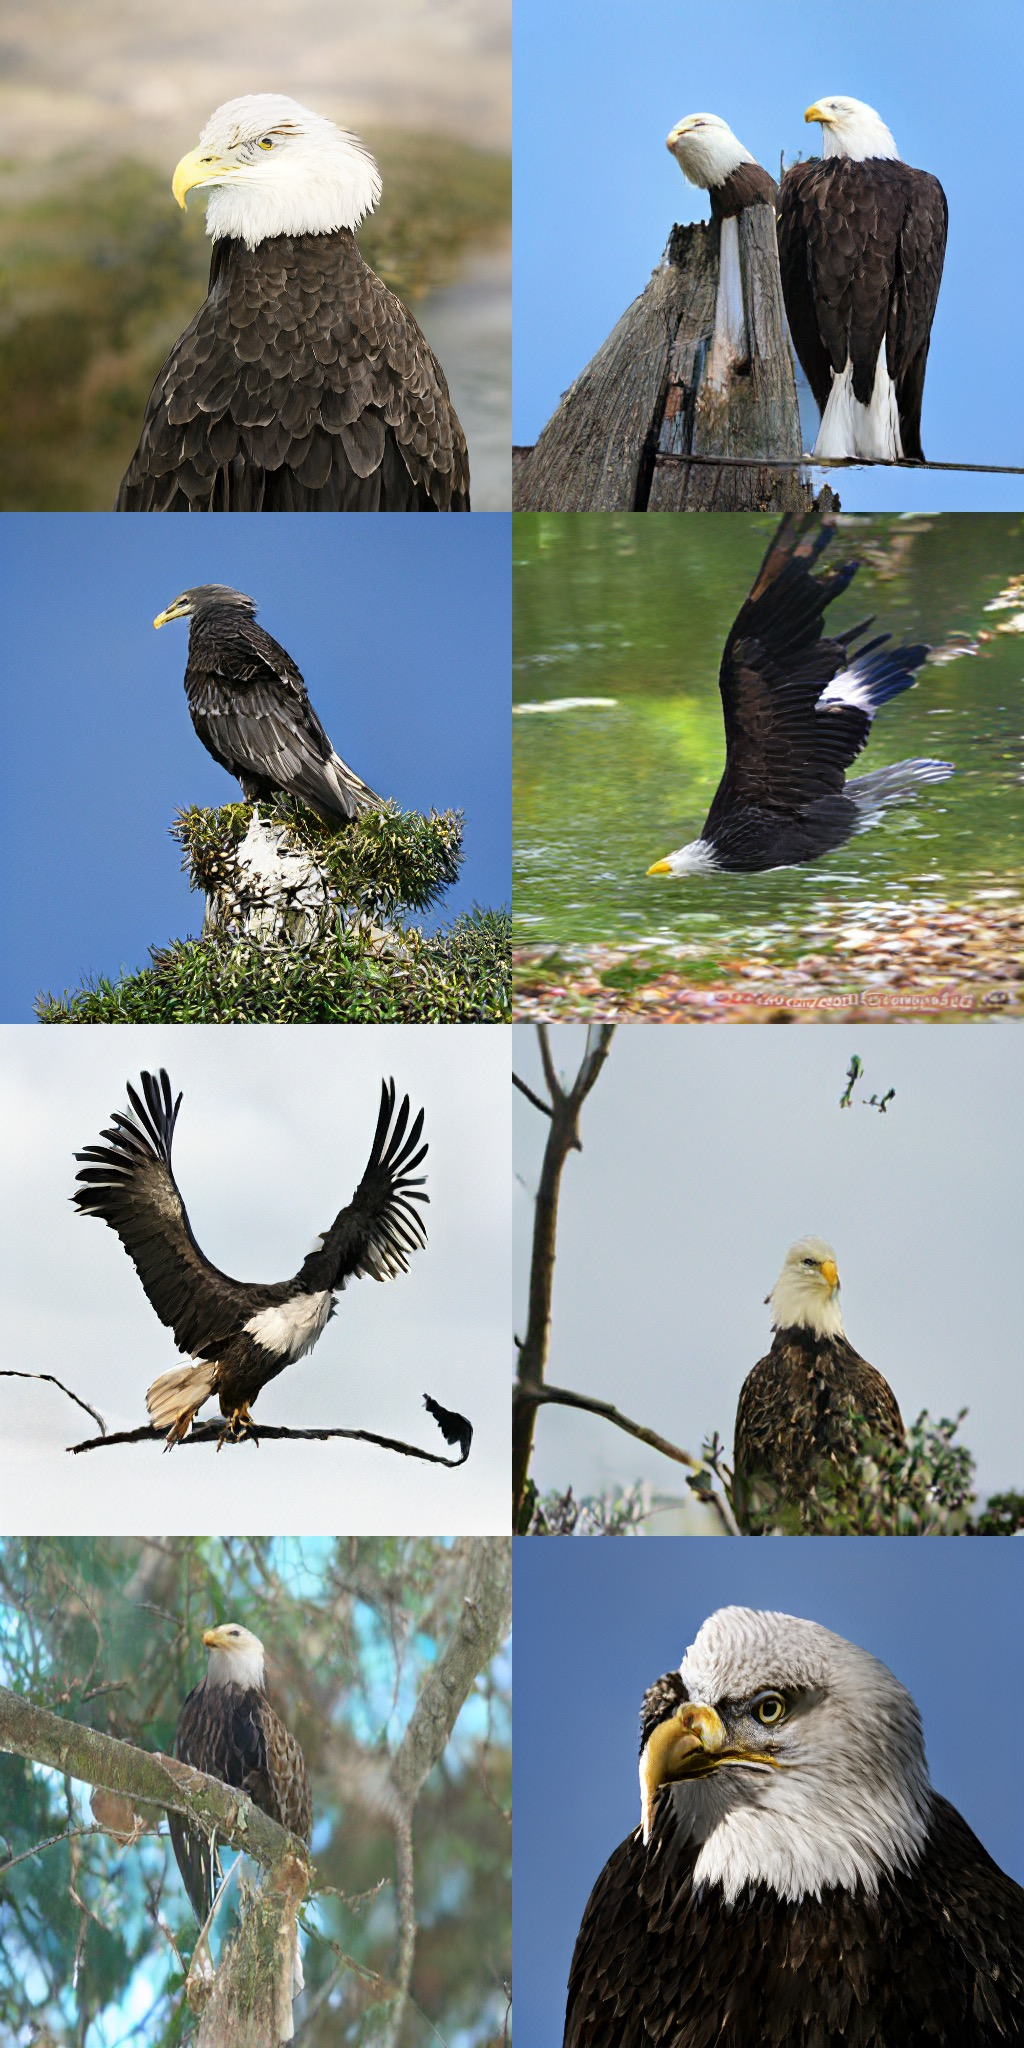
\includegraphics[ width=\tmpwidth]{figures/supp_cc/22_bald-eagle_ours.jpeg} \\ 
       
    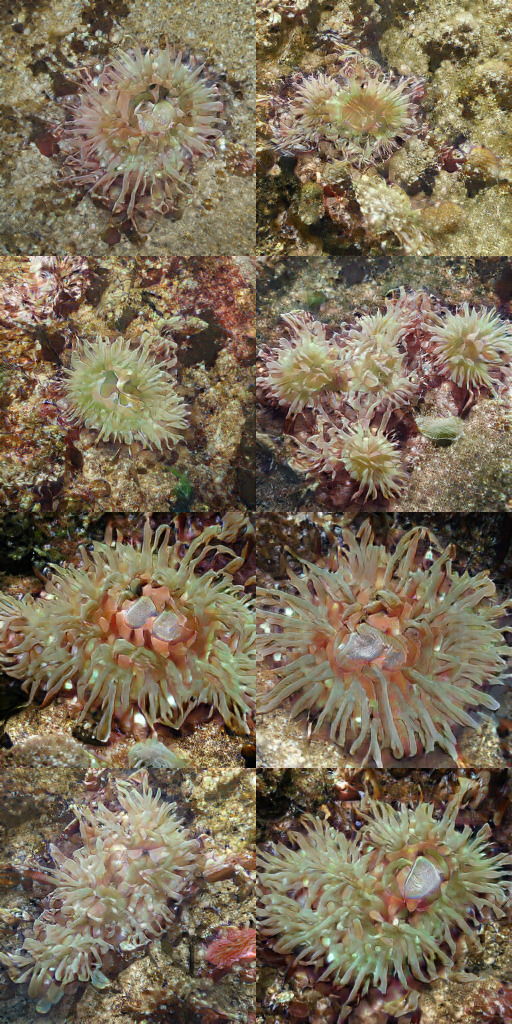
\includegraphics[ width=\tmpwidth]{figures/supp_cc/108_anemone_biggan.jpg} & \
    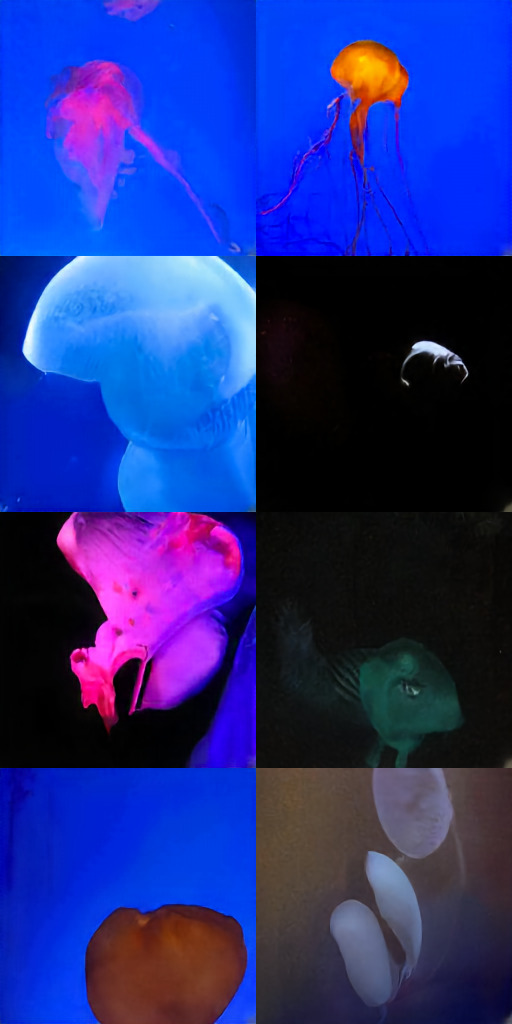
\includegraphics[ width=\tmpwidth]{figures/supp_cc/108_anemone_vqvae2.jpg}& \
    % 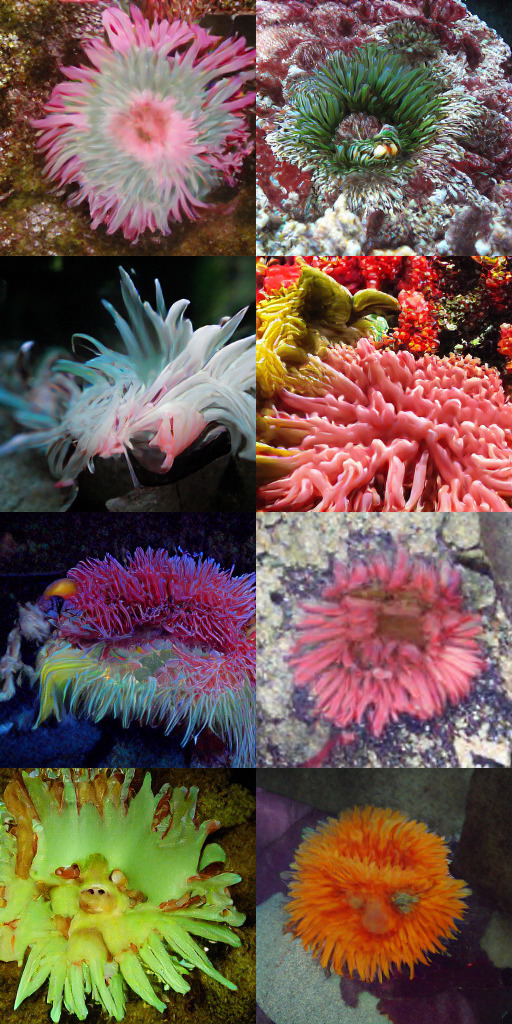
\includegraphics[ width=\tmpwidth]{figures/supp_cc/108_anemone_vqgan.jpg} & \ 
    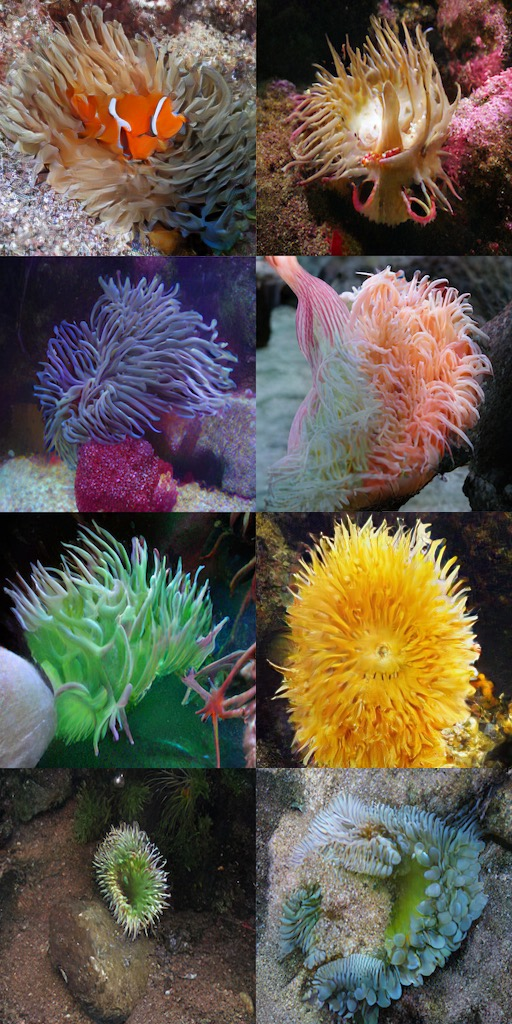
\includegraphics[ width=\tmpwidth]{figures/supp_cc/108_anemone_ours.jpeg} \\ 
    
    
    \end{tabular}
    \caption{\textbf{更多多样性比较}BigGAN-deep（截断值 1.0）、VQVAE-2\cite{Razavi19vqvae2} 和我们提出的方法 \model  在 ImageNet 上的比较。$^\dagger$ 表示从论文中提取的样本。}
    \vspace{-6mm}
    \label{fig:supp_cc_diversity}
\end{figure*}
    
\begin{figure*}[!ht]
    \centering
    \begin{tabular}{c c c}
    
    BigGAN-deep (FID=$6.95$) & VQVAE-2 (FID=$31$) & \model  (FID=\bestfid) \\
    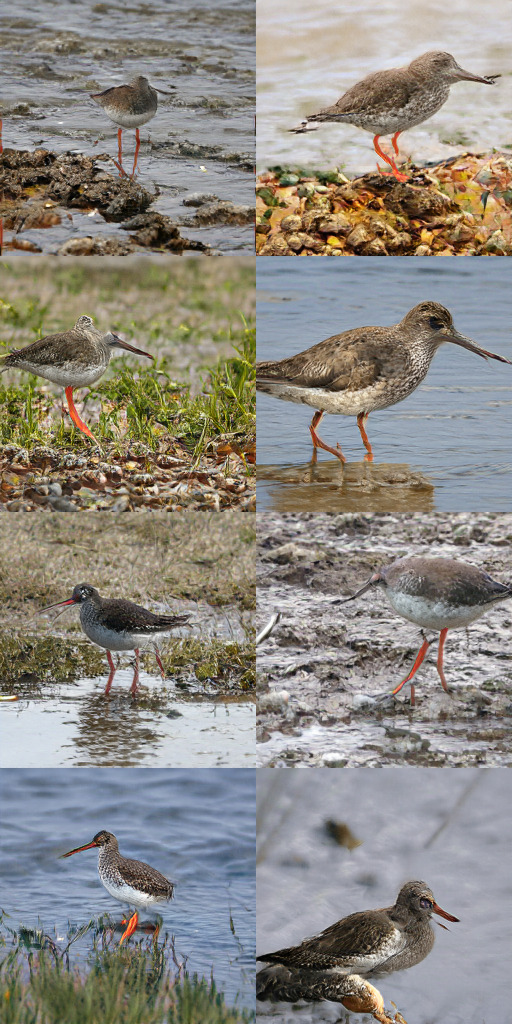
\includegraphics[ width=\tmpwidth]{figures/supp_cc/141_redshank_biggan.jpg} & \
    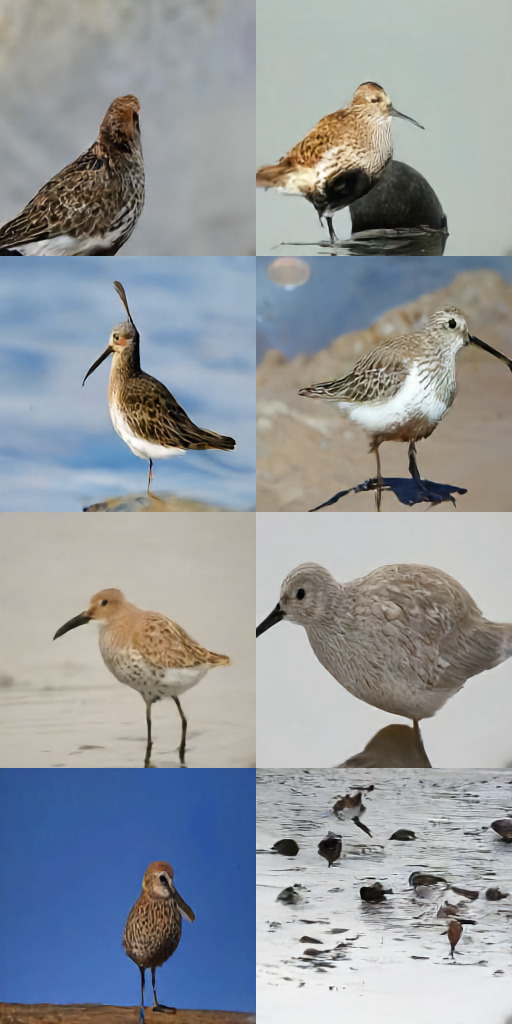
\includegraphics[ width=\tmpwidth]{figures/supp_cc/141_redshank_vqvae2.jpg}& \
    % 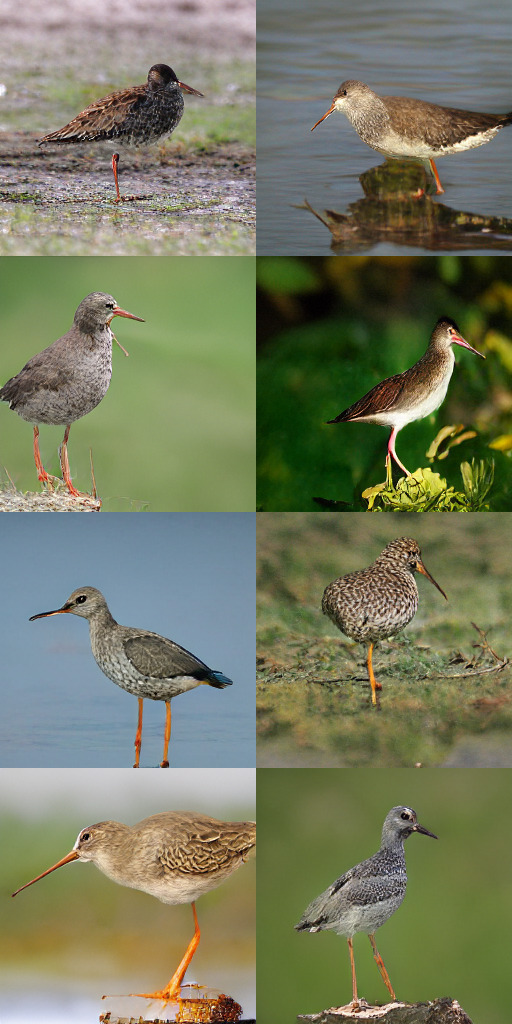
\includegraphics[ width=\tmpwidth]{figures/supp_cc/141_redshank_vqgan.jpg} & \ 
    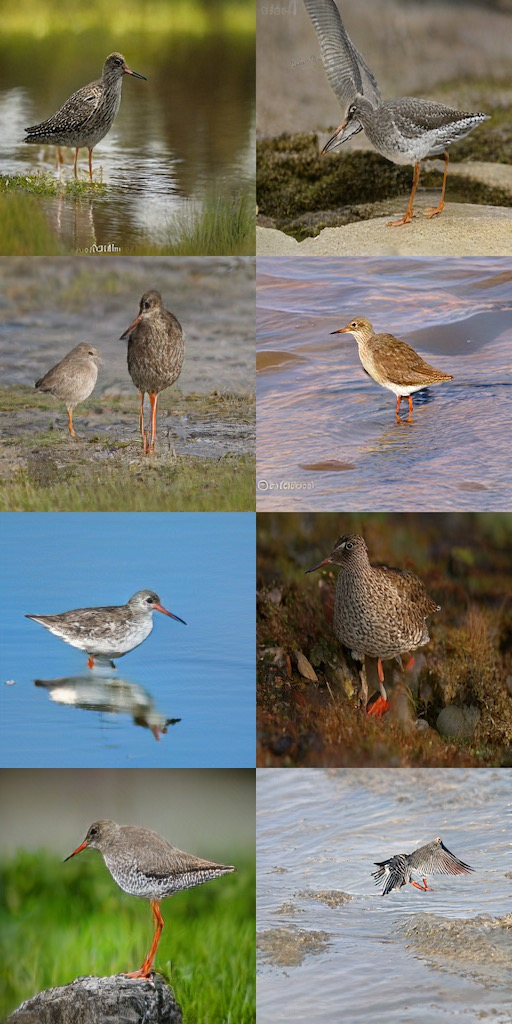
\includegraphics[ width=\tmpwidth]{figures/supp_cc/141_redshank_ours.jpeg} \\ 
    
    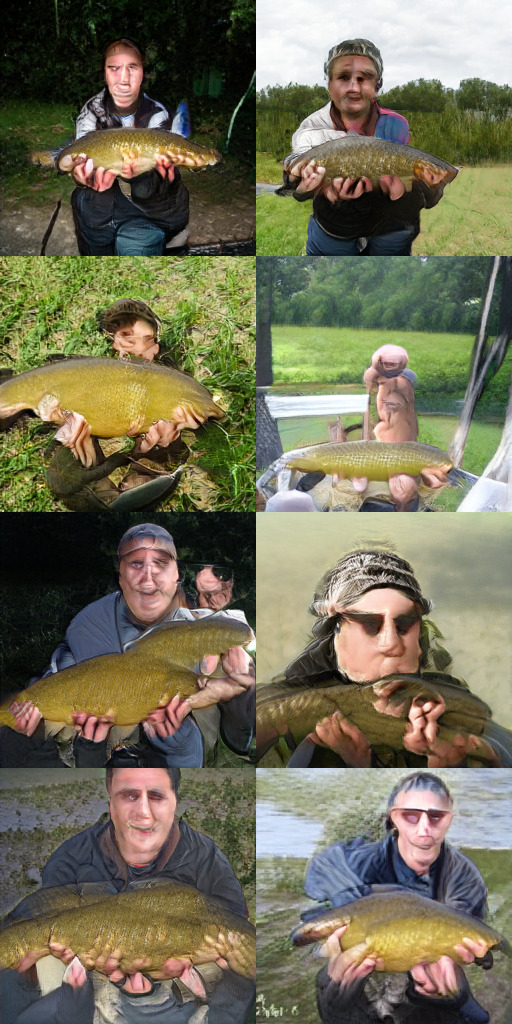
\includegraphics[ width=\tmpwidth]{figures/supp_cc/0_tench_biggan.jpg} & \
    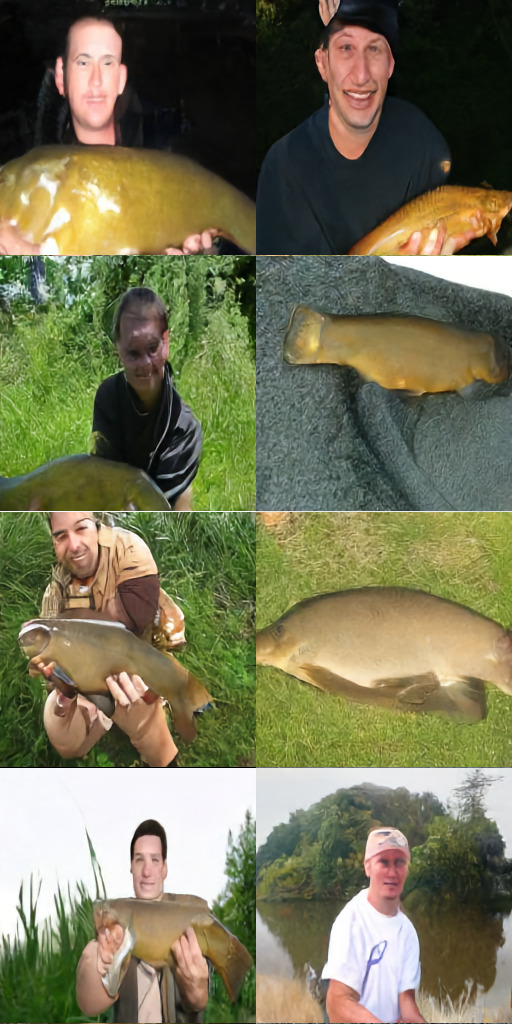
\includegraphics[ width=\tmpwidth]{figures/supp_cc/0_tench_vqvae2.jpg}& \
    % 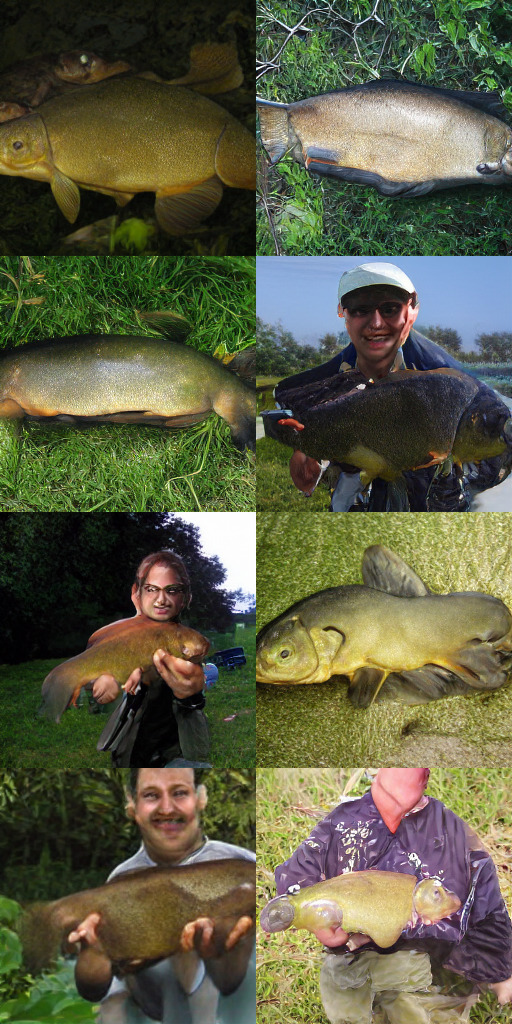
\includegraphics[ width=\tmpwidth]{figures/supp_cc/0_tench_vqgan.jpg} & \ 
    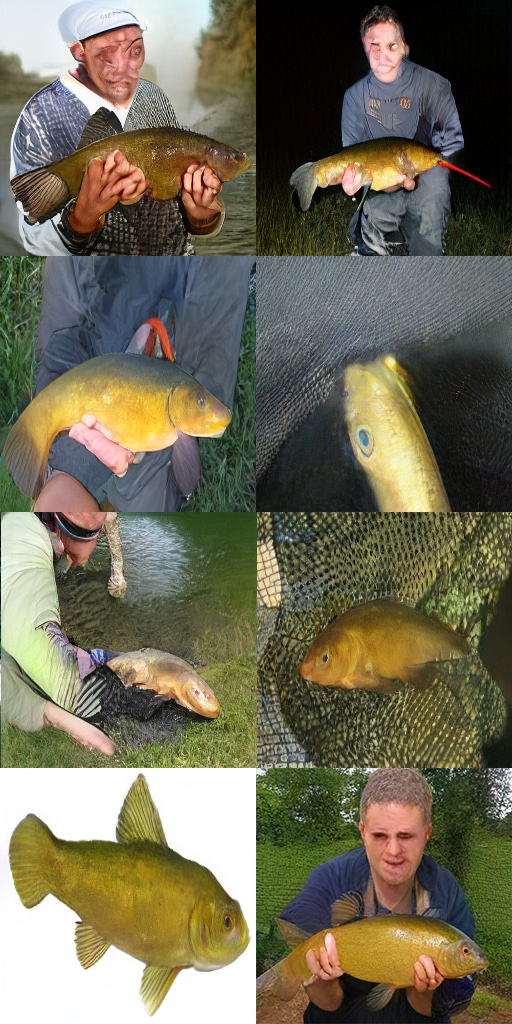
\includegraphics[ width=\tmpwidth]{figures/supp_cc/0_tench_ours.jpeg} \\ 
     
    \end{tabular}
    \caption{\textbf{更多多样性比较}BigGAN-deep（截断值 1.0）、VQVAE-2\cite{Razavi19vqvae2} 和我们提出的方法 \model  在 ImageNet 上的比较。$^\dagger$ 表示从论文中提取的样本。}
    \vspace{-6mm}
    \label{fig:supp_cc_diversity_1}
\end{figure*}   



\begin{figure*}[!ht]
    \centering
    \begin{tabular}{c c c}
    BigGAN-deep (FID=$6.95$) & VQVAE-2 (FID=$31$) & \model  (FID=\bestfid)  \\
    
    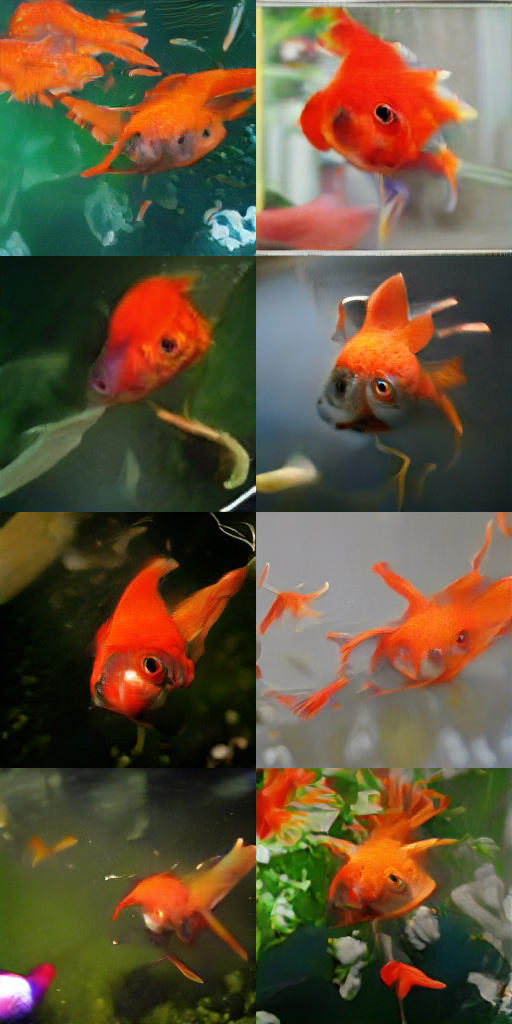
\includegraphics[ width=\tmpwidth]{figures/supp_cc/1_goldfish_biggan.jpg} & \
    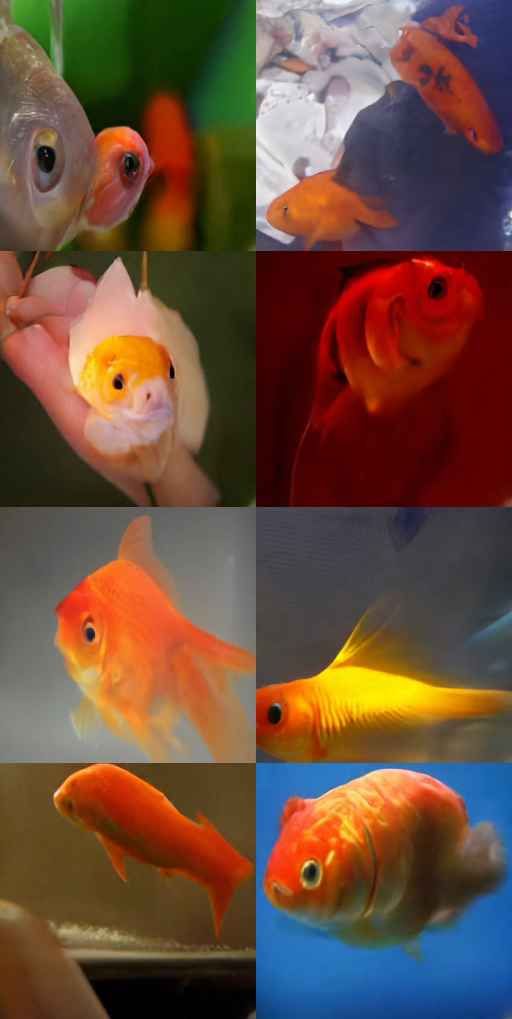
\includegraphics[ width=\tmpwidth]{figures/supp_cc/1_goldfish_vqvae2.jpg}& \
    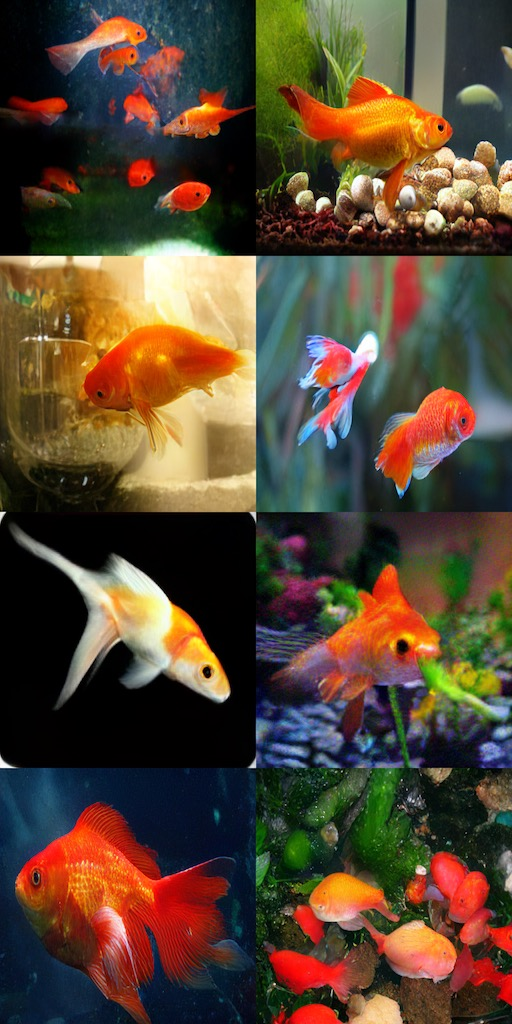
\includegraphics[ width=\tmpwidth]{figures/supp_cc/1_goldfish_ours.jpeg} \\ 
    
    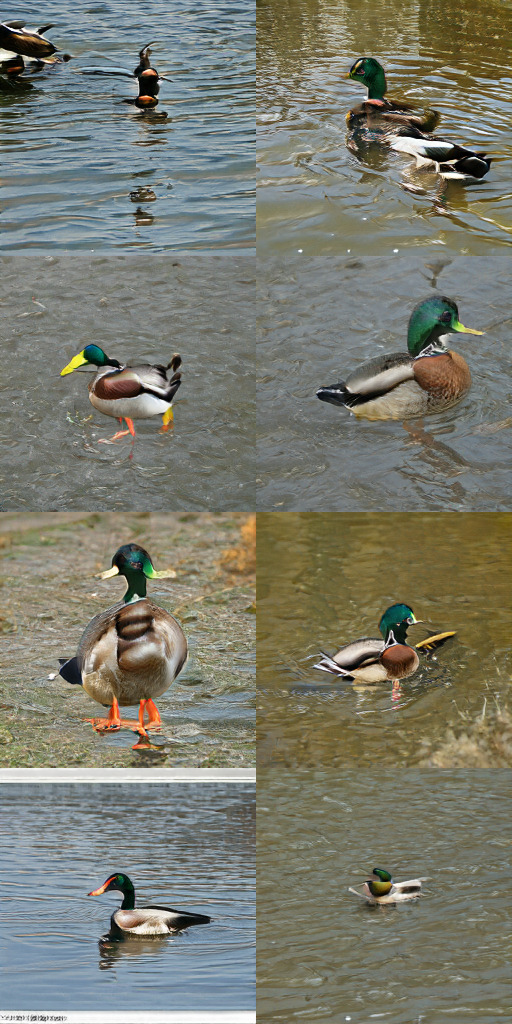
\includegraphics[ width=\tmpwidth]{figures/supp_cc/97_drake_biggan.jpg} & \
    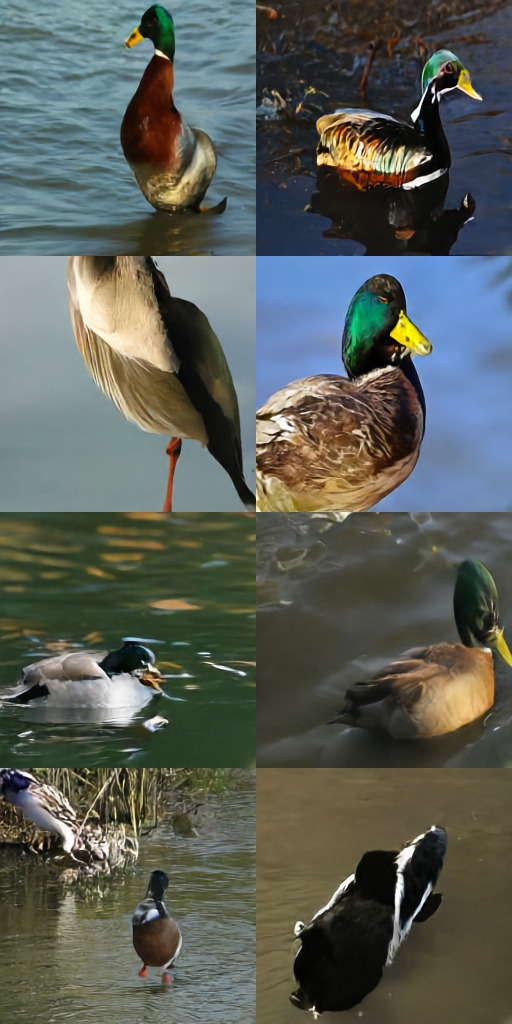
\includegraphics[ width=\tmpwidth]{figures/supp_cc/97_drake_vqvae2.jpg}& \
    % 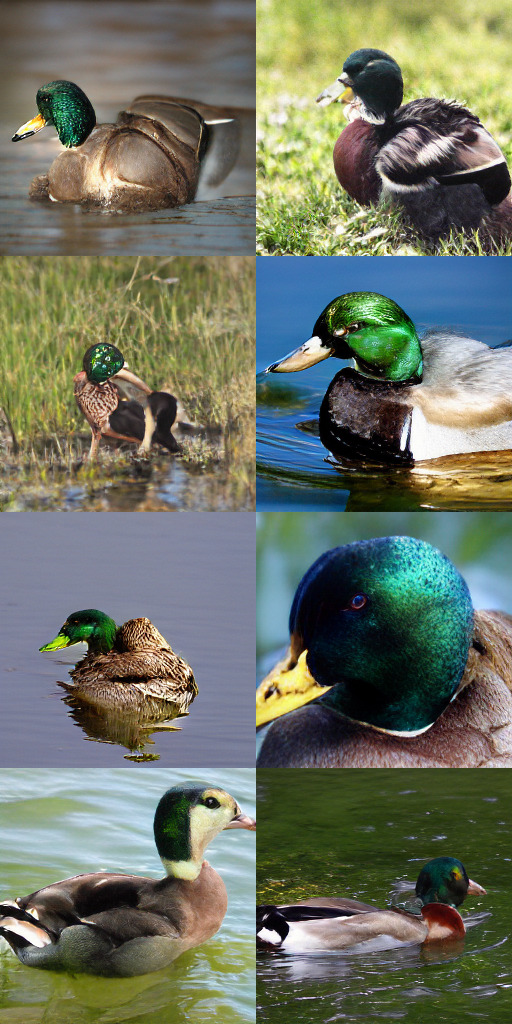
\includegraphics[ width=\tmpwidth]{figures/supp_cc/97_drake_vqgan.jpg} & \ 
    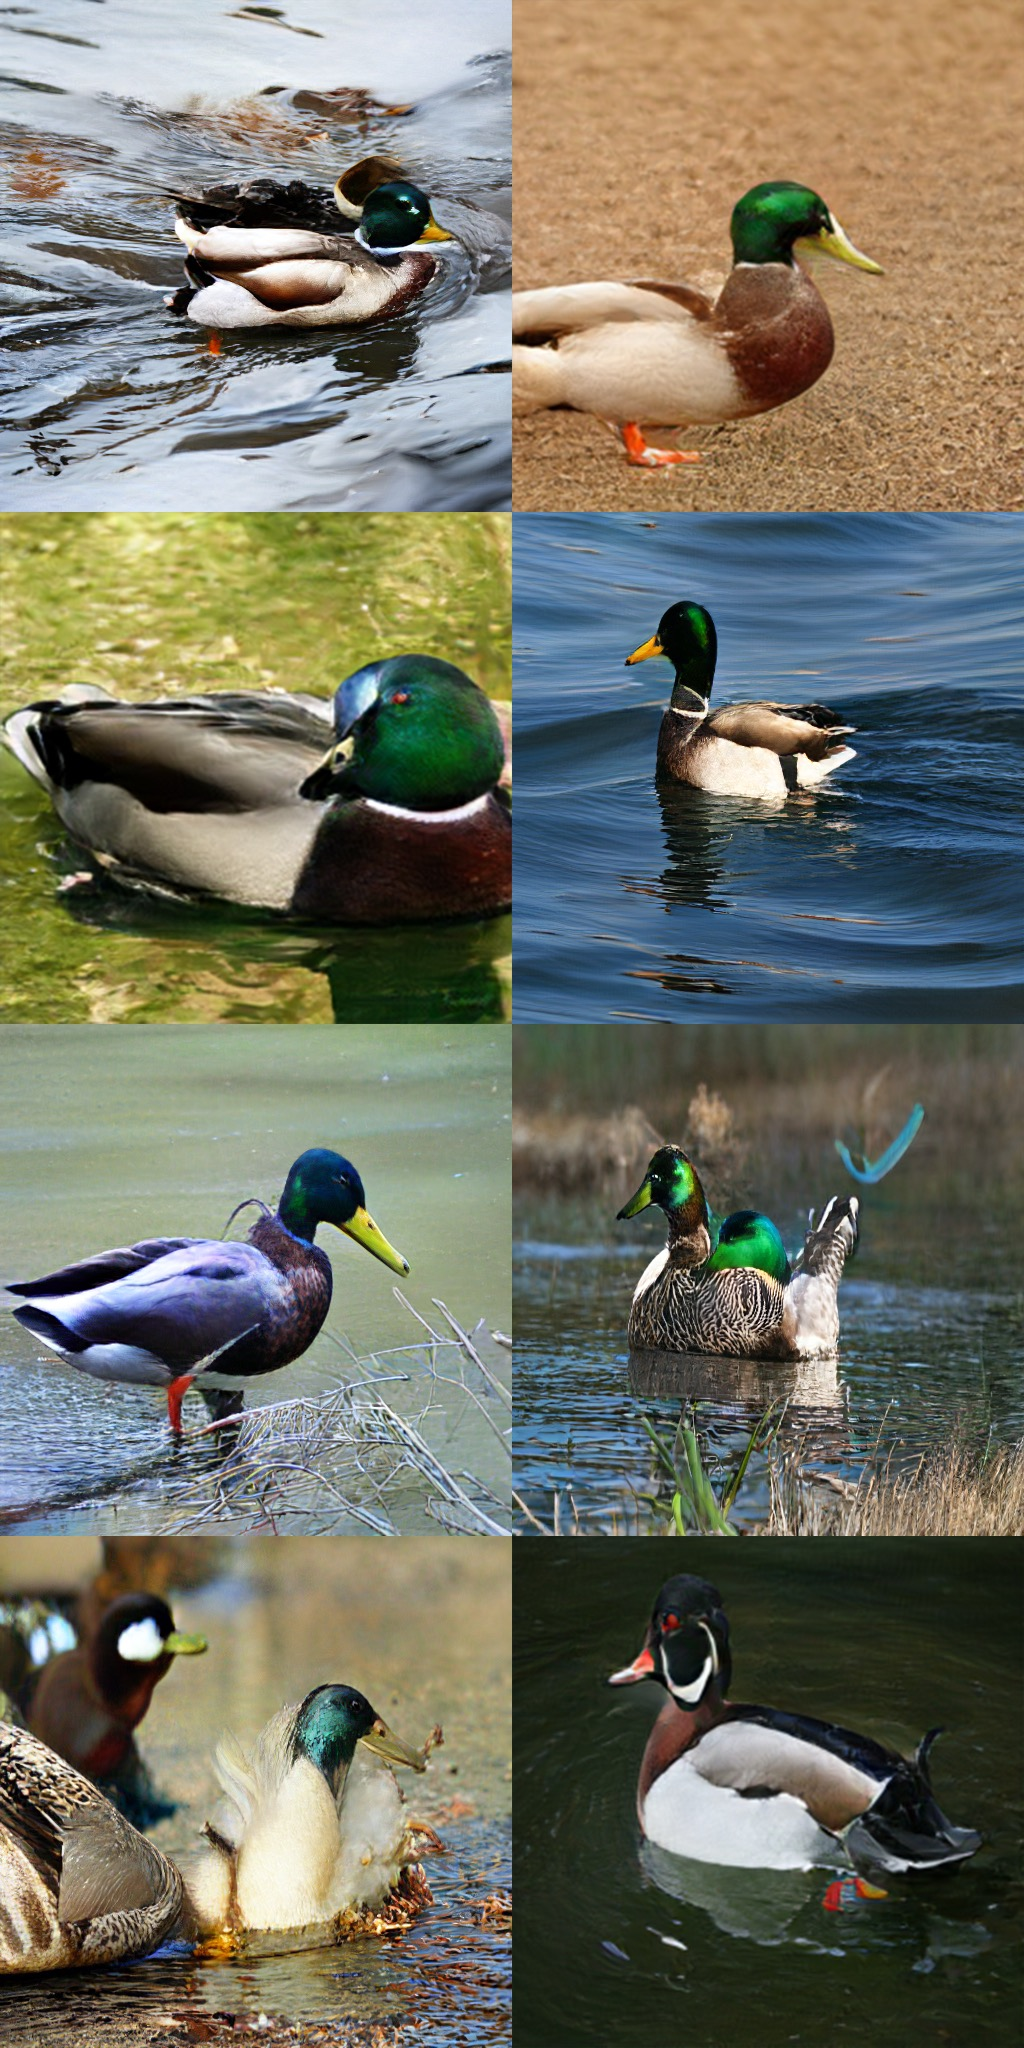
\includegraphics[ width=\tmpwidth]{figures/supp_cc/97_drake_ours.jpeg} \\ 
    
\end{tabular}
    \caption{More Diversity Comparisons among BigGAN-deep with truncation $1.0$, VQVAE-2\cite{Razavi19vqvae2}, and our proposed method \model  on ImageNet. $^\dagger$ represents extracted samples from the paper.}
    \vspace{-6mm}
    \label{fig:supp_cc_diversity_2}
\end{figure*}

\suppsection{Additional Examples of Class-conditional Image Editing Applications}
\label{sec:supp_image_editing}

\renewcommand{\tmpwidth}{28mm}

\setlength{\tabcolsep}{2pt}
\begin{figure*}[!ht]
    \centering
    %\renewcommand{\arraystretch}{2}
    \begin{tabular}{m{12mm}m{5mm} c c c c c}
Input Image &&  
\parbox[c]{\tmpwidth}{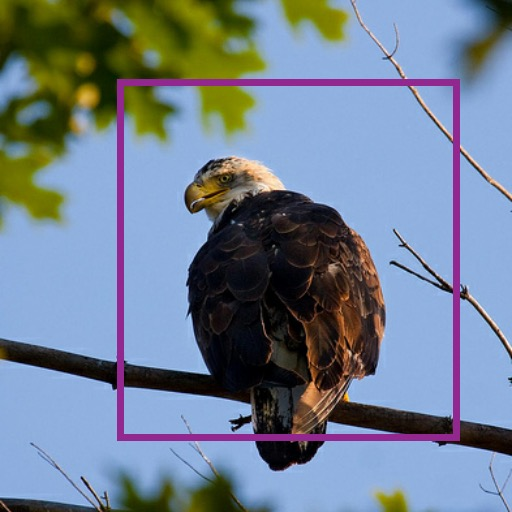
\includegraphics[ height=\tmpwidth]{figures/supp_class_modification/tree_rect.jpeg}} & 
 \parbox[c]{\tmpwidth}{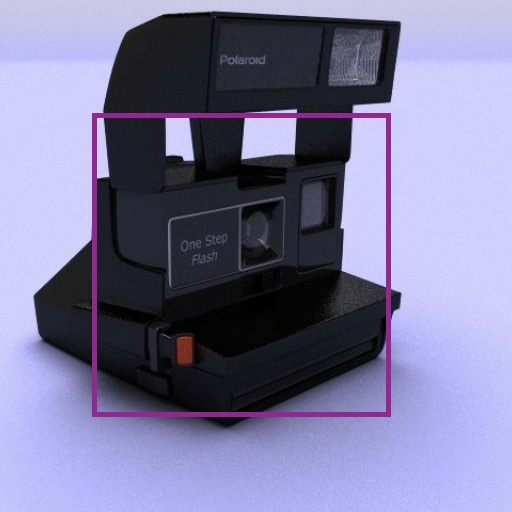
\includegraphics[ height=\tmpwidth]{figures/supp_class_modification/008784_rect.jpeg}} & 
  \parbox[c]{\tmpwidth}{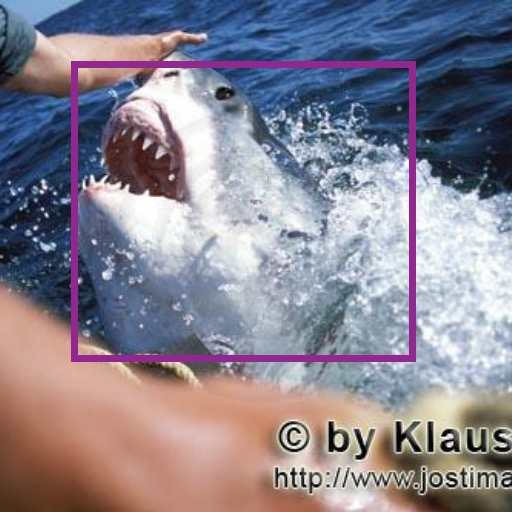
\includegraphics[ height=\tmpwidth]{figures/supp_class_modification/water_rect.jpeg}} & 
\parbox[c]{\tmpwidth}{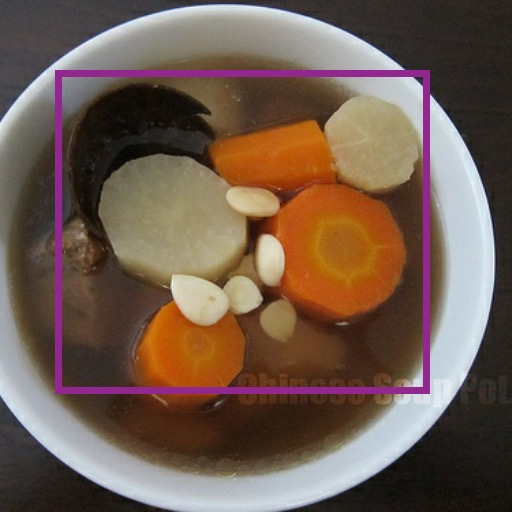
\includegraphics[ height=\tmpwidth]{figures/supp_class_modification/soup_rect.jpeg}} & 
 \parbox[c]{\tmpwidth}{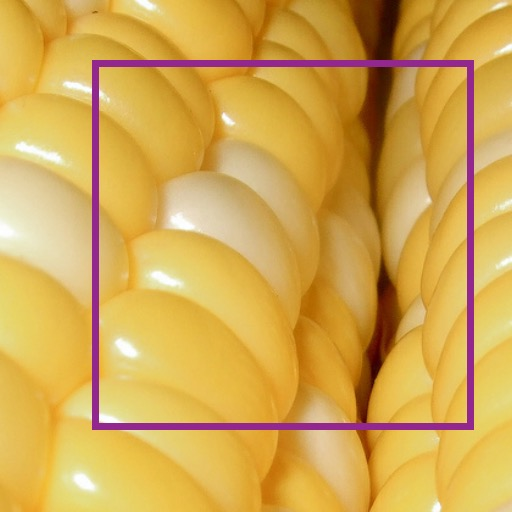
\includegraphics[ height=\tmpwidth]{figures/supp_class_modification/corn_rect.jpeg}} 
% \\ 
% Input Mask &&  
%  \parbox[c]{\tmpwidth}{\includegraphics[ width=\tmpwidth]{figures/supp_class_modification/tree_mask.jpeg}} & 
% \parbox[c]{\tmpwidth}{\includegraphics[ width=\tmpwidth]{figures/supp_class_modification/008784_mask.jpeg}} &
% \parbox[c]{\tmpwidth}{\includegraphics[ width=\tmpwidth]{figures/supp_class_modification/water_mask.jpeg}} &
%  \parbox[c]{\tmpwidth}{\includegraphics[ height=\tmpwidth]{figures/supp_class_modification/soup_mask.jpeg}} & 
%  \parbox[c]{\tmpwidth}{\includegraphics[ width=\tmpwidth]{figures/supp_class_modification/corn_mask.jpeg}} 

\\  \addlinespace[3pt]

Goldfish \texttt{[001]} && 
\parbox[c]{\tmpwidth}{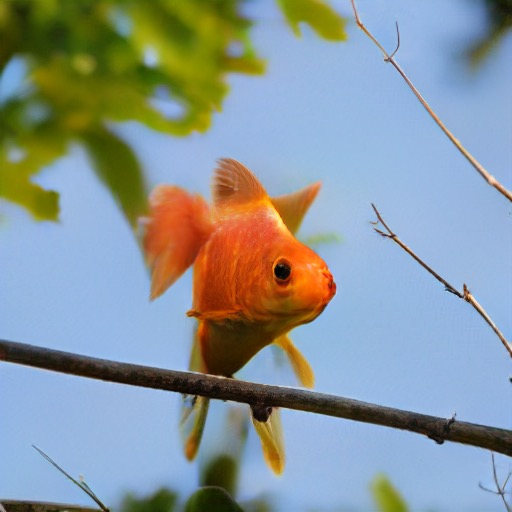
\includegraphics[ width=\tmpwidth]{figures/supp_class_modification/tree_to_001025_0018_output.jpeg}}&
\parbox[c]{\tmpwidth}{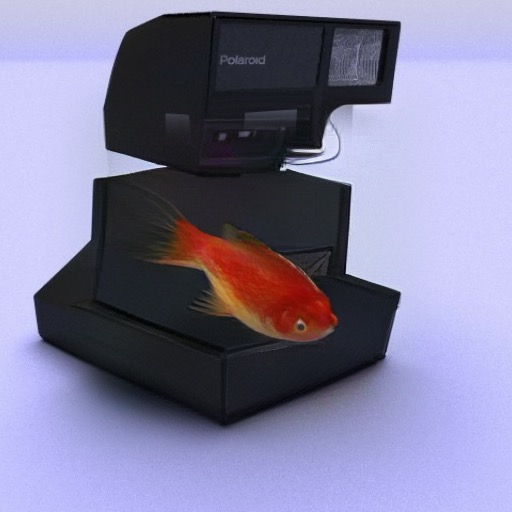
\includegraphics[ width=\tmpwidth]{figures/supp_class_modification/008784_to_001025_0001_output.jpeg}} & 
\parbox[c]{\tmpwidth}{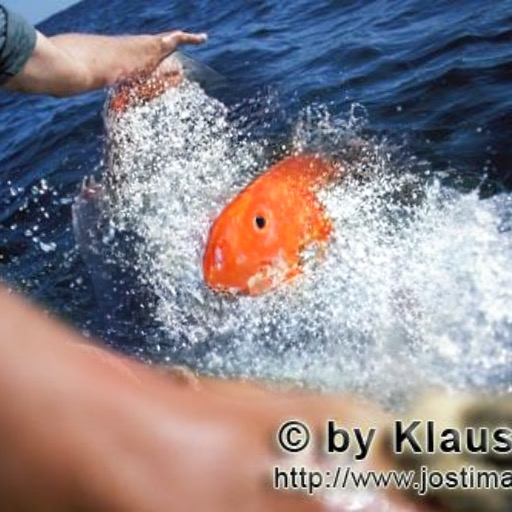
\includegraphics[ width=\tmpwidth]{figures/supp_class_modification/water1_to_001025_0000_output.jpeg}} & 
% \parbox[c]{\tmpwidth}{\includegraphics[ height=\tmpwidth]{figures/supp_class_modification/water1_to_001025_0090_output.jpeg}} & 
\parbox[c]{\tmpwidth}{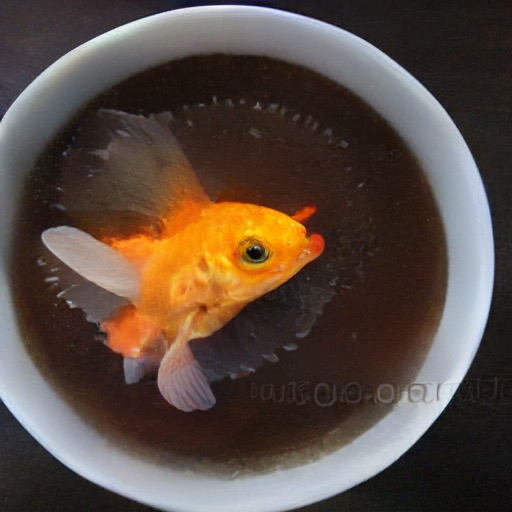
\includegraphics[ height=\tmpwidth]{figures/supp_class_modification/soup_to_001025_0012_output.jpeg}} & 
\parbox[c]{\tmpwidth}{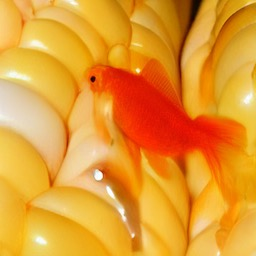
\includegraphics[ width=\tmpwidth]{figures/supp_class_modification/000398_to_001025_0002_output.jpeg}} 

\\

Ice Bear \texttt{[296]} && 
\parbox[c]{\tmpwidth}{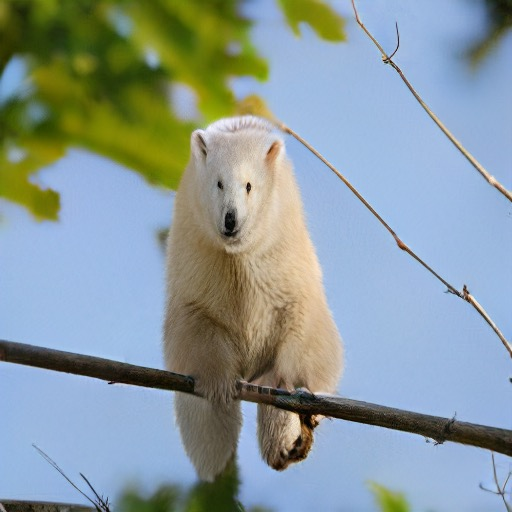
\includegraphics[ width=\tmpwidth]{figures/supp_class_modification/tree_to_001320_0004_output.jpeg}} & 
\parbox[c]{\tmpwidth}{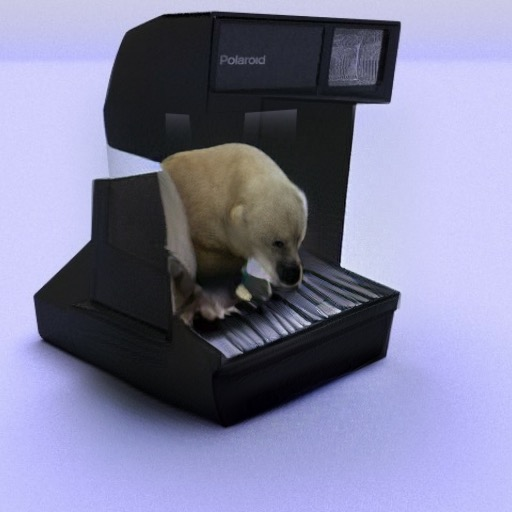
\includegraphics[ width=\tmpwidth]{figures/supp_class_modification/008784_to_001320_0002_output.jpeg}} & 
\parbox[c]{\tmpwidth}{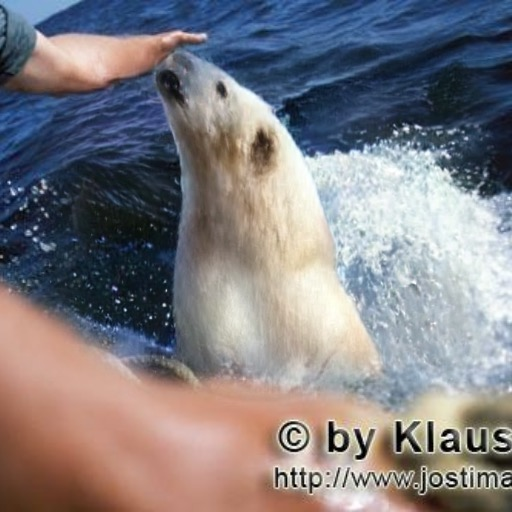
\includegraphics[ width=\tmpwidth]{figures/supp_class_modification/water_to_001320_0005_output.jpeg}} & 
\parbox[c]{\tmpwidth}{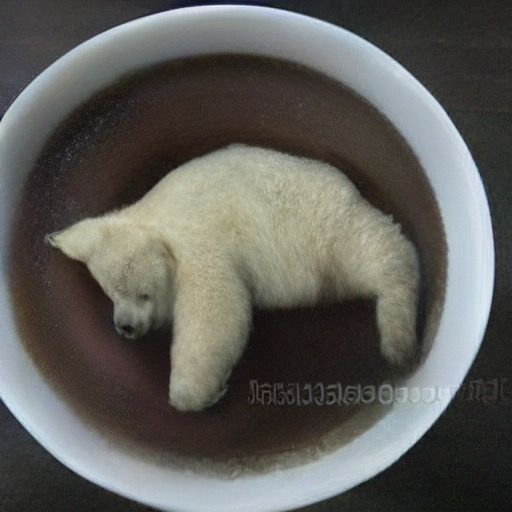
\includegraphics[ height=\tmpwidth]{figures/supp_class_modification/soup_to_001320_0008_output.jpeg}} & 
\parbox[c]{\tmpwidth}{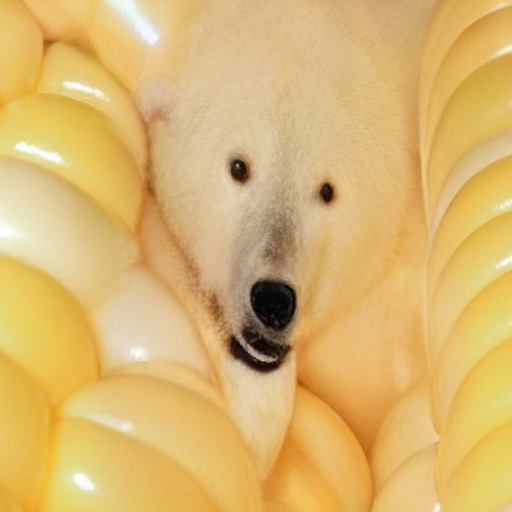
\includegraphics[ width=\tmpwidth]{figures/supp_class_modification/corn_to_001320_0025_output.jpeg}} 
\\
Argaric 
\texttt{[992]} &&
\parbox[c]{\tmpwidth}{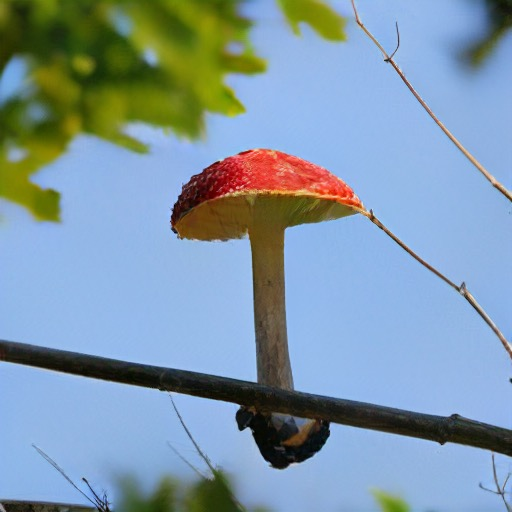
\includegraphics[ width=\tmpwidth]{figures/supp_class_modification/tree_to_002016_0006_output.jpeg}} & 
\parbox[c]{\tmpwidth}{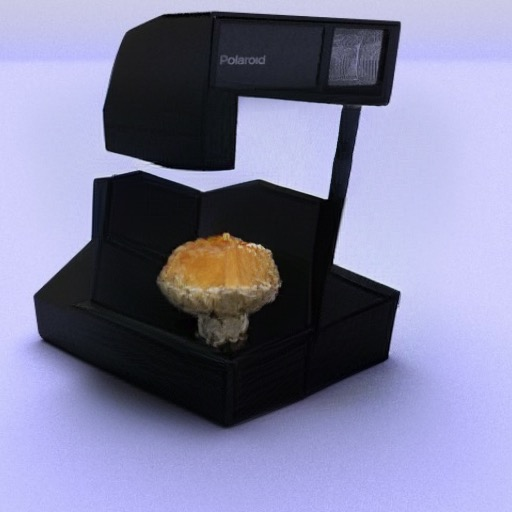
\includegraphics[ width=\tmpwidth]{figures/supp_class_modification/008784_to_002016_0003_output.jpeg}} & 
\parbox[c]{\tmpwidth}{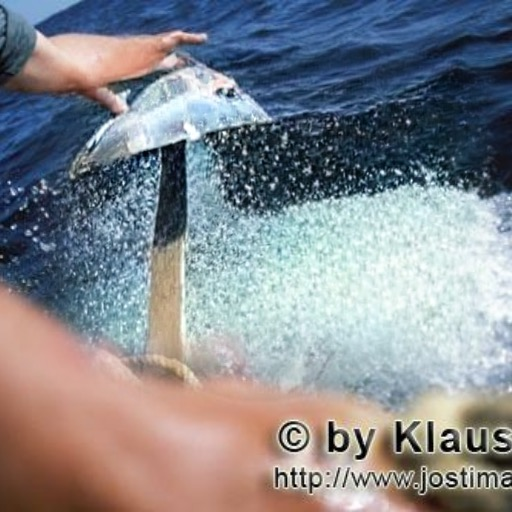
\includegraphics[ width=\tmpwidth]{figures/supp_class_modification/water_to_002016_0009_output.jpeg}} & 
\parbox[c]{\tmpwidth}{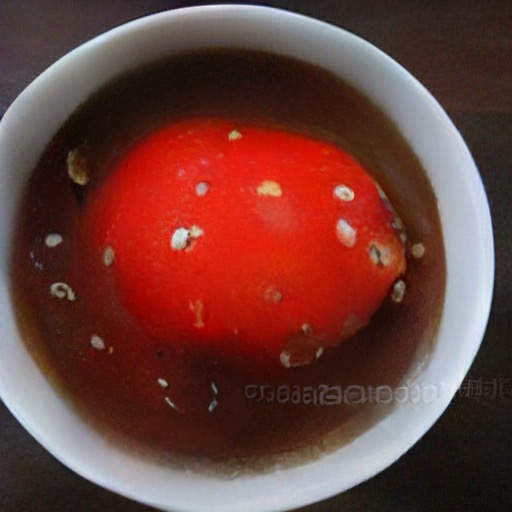
\includegraphics[ height=\tmpwidth]{figures/supp_class_modification/soup_to_002016_0000_output.jpeg}} & 
\parbox[c]{\tmpwidth}{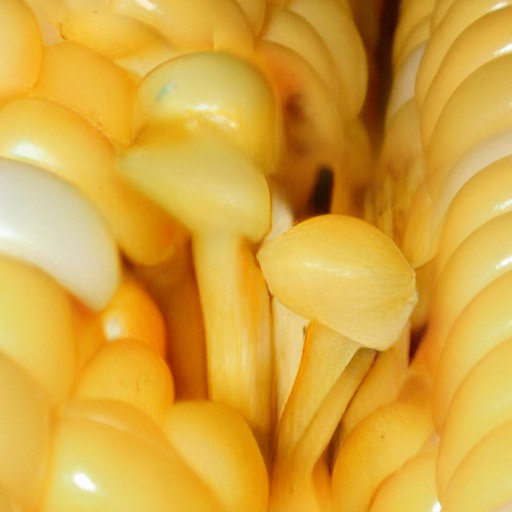
\includegraphics[ width=\tmpwidth]{figures/supp_class_modification/corn_to_001971_0011_output.jpeg}} 

\\

Lorikeet 
\texttt{[90]} &&
 \parbox[c]{\tmpwidth}{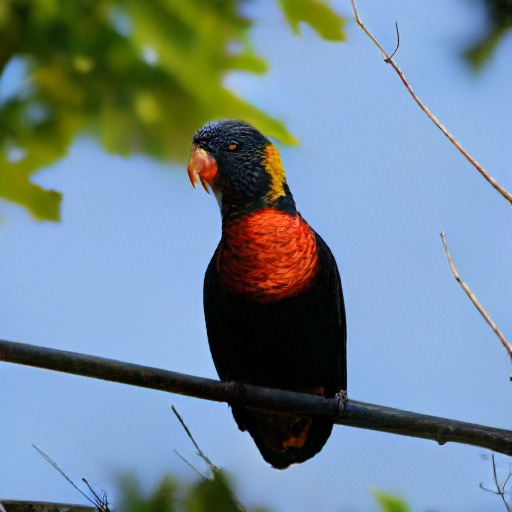
\includegraphics[ width=\tmpwidth]{figures/supp_class_modification/tree_to_001114_0005_output.jpeg}} & 
  \parbox[c]{\tmpwidth}{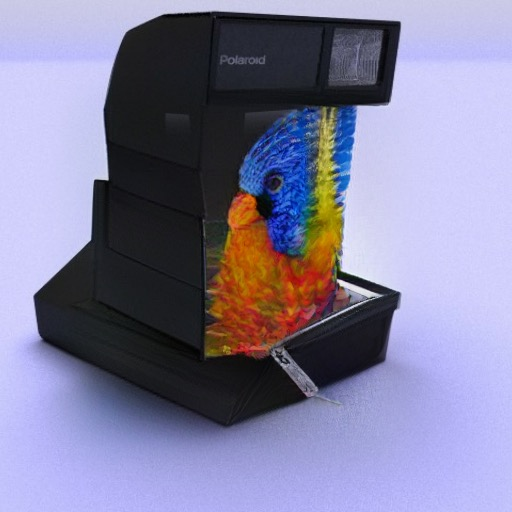
\includegraphics[ width=\tmpwidth]{figures/supp_class_modification/008784_to_001114_0003_output.jpeg}} & 
   \parbox[c]{\tmpwidth}{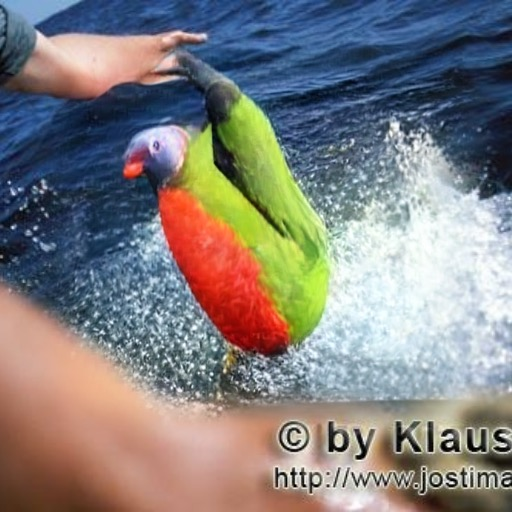
\includegraphics[ width=\tmpwidth]{figures/supp_class_modification/water_to_001114_0007_output.jpeg}} & 
 \parbox[c]{\tmpwidth}{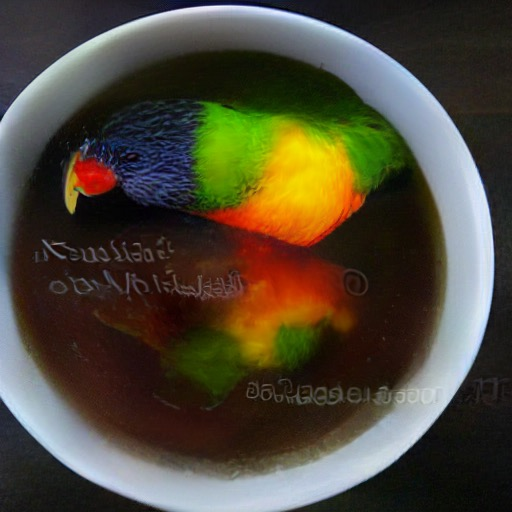
\includegraphics[ height=\tmpwidth]{figures/supp_class_modification/soup_to_001114_0009_output.jpeg}} & 
 \parbox[c]{\tmpwidth}{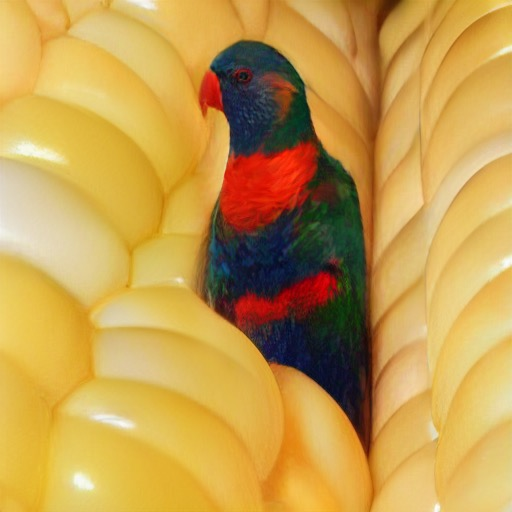
\includegraphics[ width=\tmpwidth]{figures/supp_class_modification/corn_to_001114_0015_output.jpeg}}

\\


% Red Fox \texttt{[145]} && 
%  \parbox[c]{\tmpwidth}{\includegraphics[ width=\tmpwidth]{figures/supp_class_modification/008857_to_001301_0000_output.jpeg}} & 
%  \parbox[c]{\tmpwidth}{\includegraphics[ width=\tmpwidth]{figures/supp_class_modification/000398_to_001303_0006_output.jpeg}} & 
%  \parbox[c]{\tmpwidth}{\includegraphics[ width=\tmpwidth]{figures/supp_class_modification/008784_to_001301_0003_output.jpeg}} & 
% \\


Train \texttt{[829]} && 
\parbox[c]{\tmpwidth}{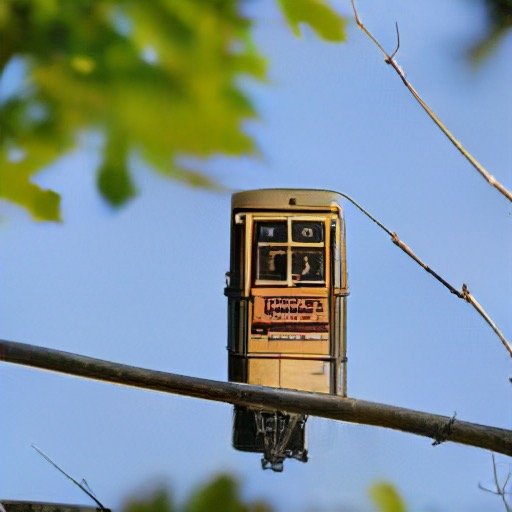
\includegraphics[ width=\tmpwidth]{figures/supp_class_modification/tree_to_001853_0015_output.jpeg}} & 
\parbox[c]{\tmpwidth}{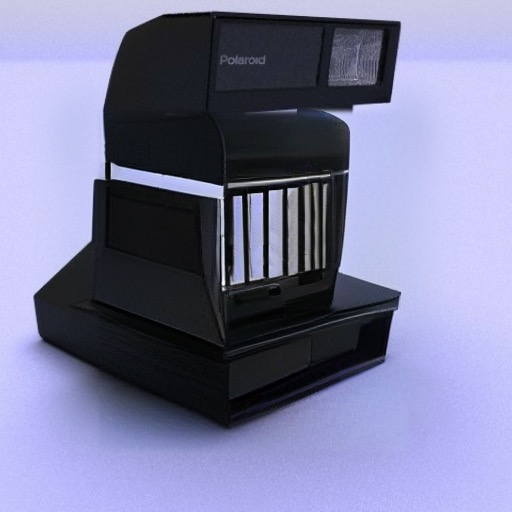
\includegraphics[ width=\tmpwidth]{figures/supp_class_modification/008784_to_001853_0004_output.jpeg}} & 
\parbox[c]{\tmpwidth}{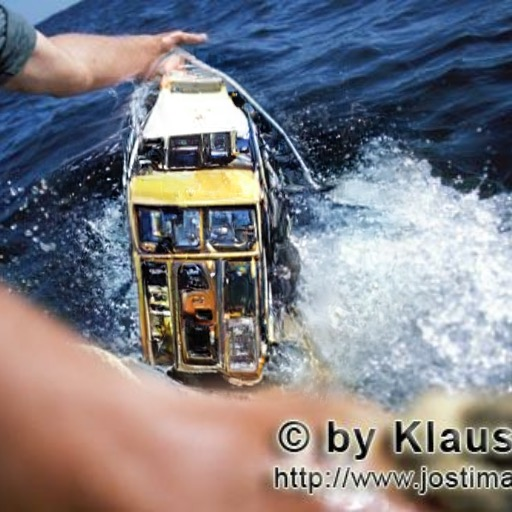
\includegraphics[ width=\tmpwidth]{figures/supp_class_modification/water_to_001853_0016_output.jpeg}} & 
\parbox[c]{\tmpwidth}{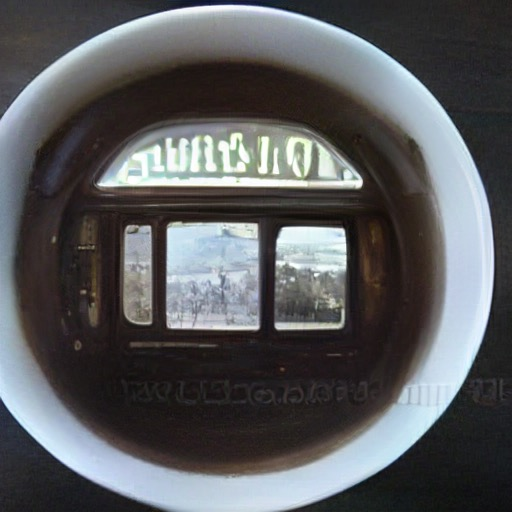
\includegraphics[ height=\tmpwidth]{figures/supp_class_modification/soup_to829_0002_output.jpeg}} & 
\parbox[c]{\tmpwidth}{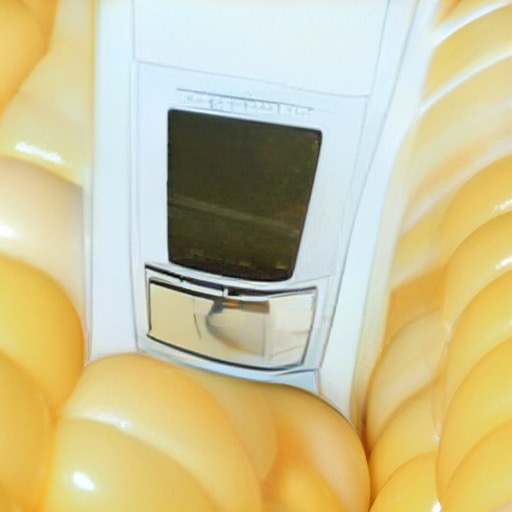
\includegraphics[ width=\tmpwidth]{figures/supp_class_modification/corn_to_001853_0111_output.jpeg}} 
\\



Tiger 
\texttt{[292]} && 
\parbox[c]{\tmpwidth}{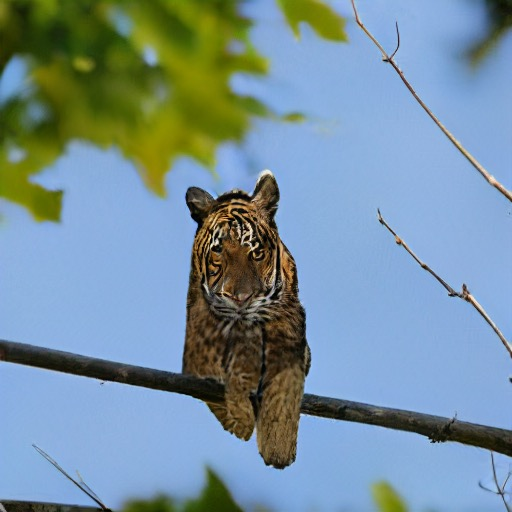
\includegraphics[ width=\tmpwidth]{figures/supp_class_modification/tree_to_001316_0004_output.jpeg}}&
\parbox[c]{\tmpwidth}{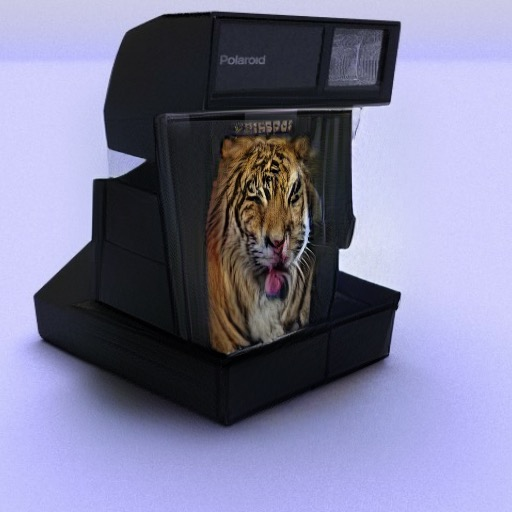
\includegraphics[ width=\tmpwidth]{figures/supp_class_modification/008784_to_001316_0002_output.jpeg}} & 
\parbox[c]{\tmpwidth}{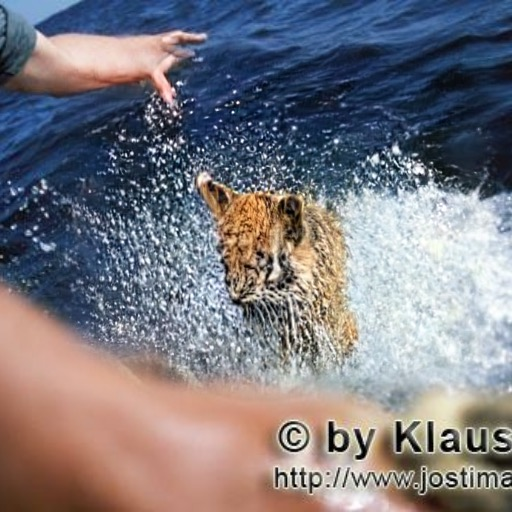
\includegraphics[ width=\tmpwidth]{figures/supp_class_modification/water_to_292_0000_output.jpeg}} & 
\parbox[c]{\tmpwidth}{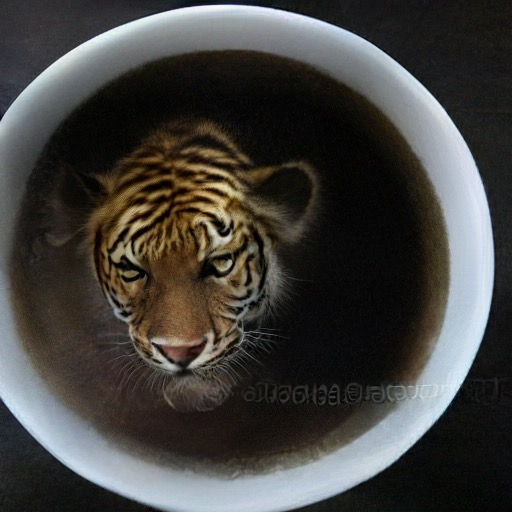
\includegraphics[ height=\tmpwidth]{figures/supp_class_modification/soup_to_001316_0014_output.jpeg}} & 
\parbox[c]{\tmpwidth}{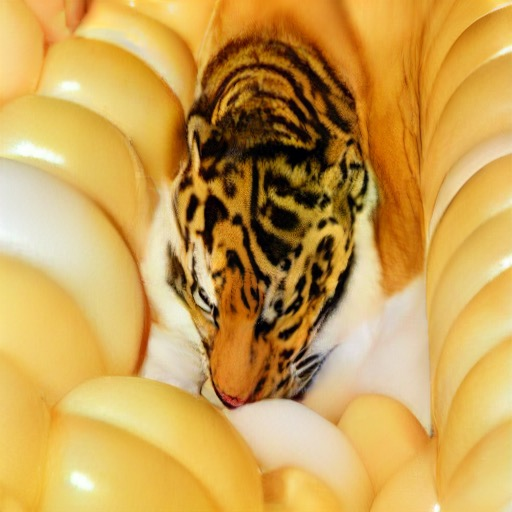
\includegraphics[ width=\tmpwidth]{figures/supp_class_modification/corn_to_001316_0105_output.jpeg}} 

\\

%  \parbox[c]{\tmpwidth}{\includegraphics[ width=\tmpwidth]{figures/supp_class_modification/000398_to_001320_0002_output.jpeg}} & 
%  \parbox[c]{\tmpwidth}{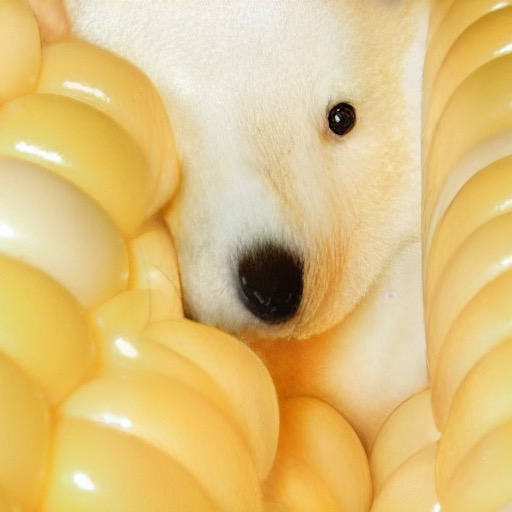
\includegraphics[ width=\tmpwidth]{figures/supp_class_modification/corn_to_001320_0018_output.jpeg}} &


    \end{tabular}
    \caption{\textbf{More Examples of Class-conditional Image Editing.} In each column, the bottom images are synthesized using the image on the top, ImageNet class labels on the left, and a bounding box of the main object downsampled into latent space (as shown in the second row).}
    \vspace{-12mm}
    \label{fig:supp_editing}
\end{figure*}


% \begin{figure*}[!ht]
%     \centering
%     %\renewcommand{\arraystretch}{2}
%     \begin{tabular}{m{12mm}m{5mm} c c c c}

% Input Image &&  
%  \parbox[c]{\tmpwidth}{\includegraphics[ height=\tmpwidth]{figures/supp_class_modification/003999_input.jpeg}} & 
%  \parbox[c]{\tmpwidth}{\includegraphics[ height=\tmpwidth]{figures/supp_class_modification/008784_input.jpeg}} & 
% \\ 

% Input Mask &&  
%  \parbox[c]{\tmpwidth}{\includegraphics[ width=\tmpwidth]{figures/supp_class_modification/003999_mask.jpeg}} & 
%  \parbox[c]{\tmpwidth}{\includegraphics[ width=\tmpwidth]{figures/supp_class_modification/008784_mask.jpeg}} &
 
% \\  \addlinespace[3pt]

% Penguin 
% \texttt{[145]} && 
%  \parbox[c]{\tmpwidth}{\includegraphics[ width=\tmpwidth]{figures/supp_class_modification/003999_to145_0000_output.jpeg}} & 
% \\

% Pineapple 
% \texttt{[145]} && 
%  \parbox[c]{\tmpwidth}{\includegraphics[ width=\tmpwidth]{figures/supp_class_modification/003999_to_000036_0009_output.jpeg}} & 
% \\

% Ice Bear
% \texttt{[145]} && 
%  \parbox[c]{\tmpwidth}{\includegraphics[ width=\tmpwidth]{figures/supp_class_modification/003999_to_000663_0007_output.jpeg}} & 
% \\

% Red Fox 
% \texttt{[145]} && 
%  \parbox[c]{\tmpwidth}{\includegraphics[ width=\tmpwidth]{figures/supp_class_modification/003999_to_000601_0009_output.jpeg}} & 
% \\

% Owl
% \texttt{[145]} && 
%  \parbox[c]{\tmpwidth}{\includegraphics[ width=\tmpwidth]{figures/supp_class_modification/003999_to_000036_0004_output.jpeg}} & 
% \\

% \end{tabular}
%     \caption{More Sample Diversity Comparisons for BigGAN-deep with truncation $1.0$ and our proposed method \model on ImageNet.}
%     \vspace{-6mm}
%     \label{fig:supp_diversity}
% \end{figure*}
\renewcommand{\tmpwidth}{32mm}
\setlength{\tabcolsep}{2pt}
\begin{figure*}[!ht]
    \centering
    %\renewcommand{\arraystretch}{2}
    \begin{tabular}{cc}
% \includegraphics[ height=\tmpwidth]{figures/panorama/000020_ours.jpeg} \\ 
Input & \model (Ours)
\\ 

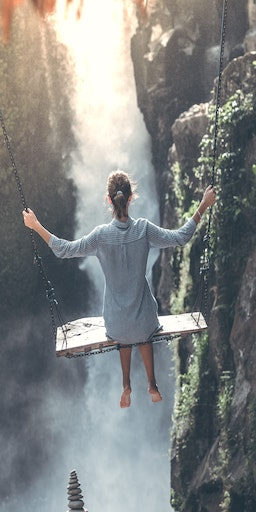
\includegraphics[ height=\tmpwidth]{figures/panorama/artem-beliaikin-8AsKha7aIvk-unsplash.jpg} &
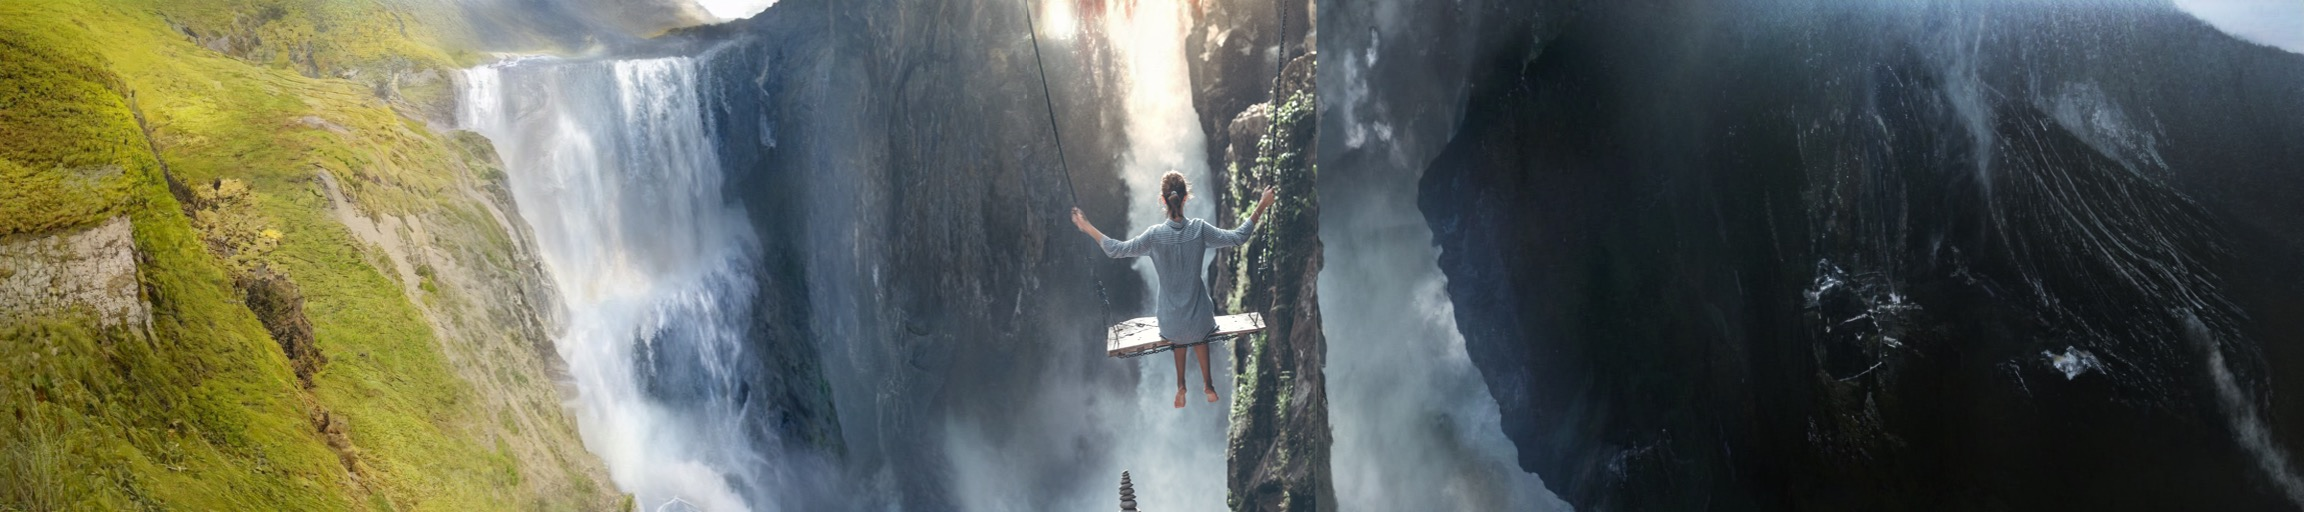
\includegraphics[ height=\tmpwidth]{figures/panorama/artem-beliaikin-8AsKha7aIvk-unsplash_ours.jpeg} \\ 


% \includegraphics[ height=\tmpwidth]{figures/panorama/damiano-baschiera-hFXZ5cNfkOk-unsplash.jpg_input.jpeg} \\ 
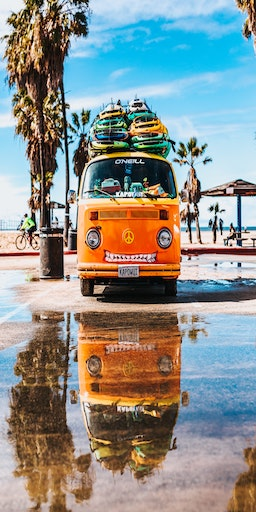
\includegraphics[ height=\tmpwidth]{figures/panorama/tyler-nix-6mze64HRU2Q-unsplash.jpg} &
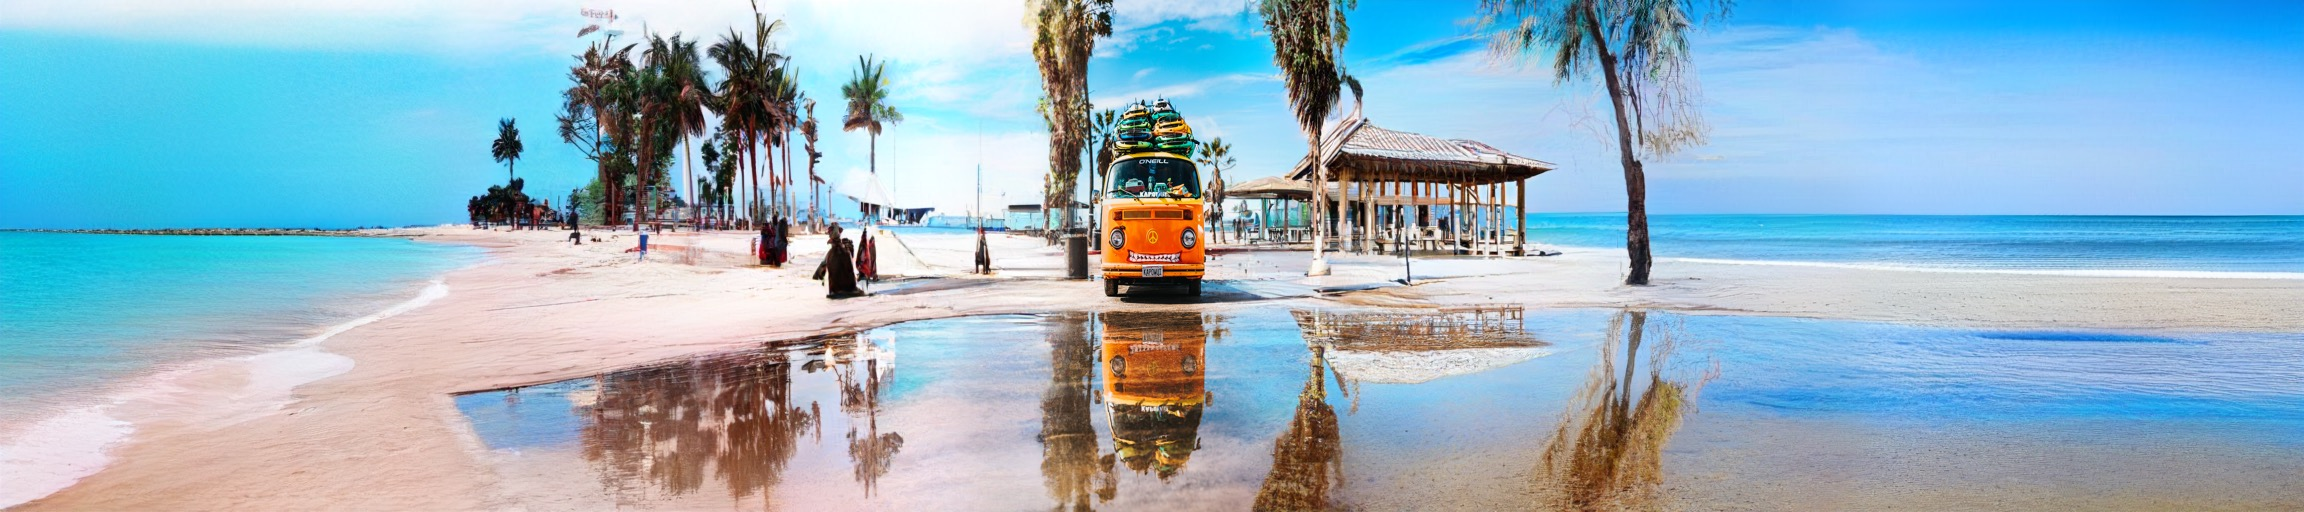
\includegraphics[ height=\tmpwidth]{figures/panorama/tyler-nix-6mze64HRU2Q-unsplash_panorama.jpeg} \\ 
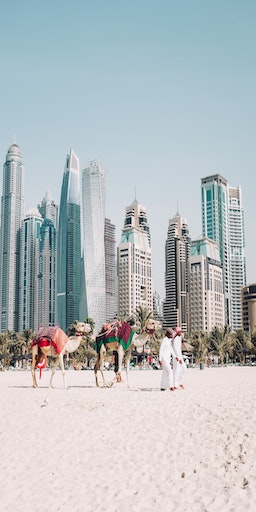
\includegraphics[ height=\tmpwidth]{figures/panorama/fredrik-ohlander-fCW1hWq2nq0-unsplash.jpg} &
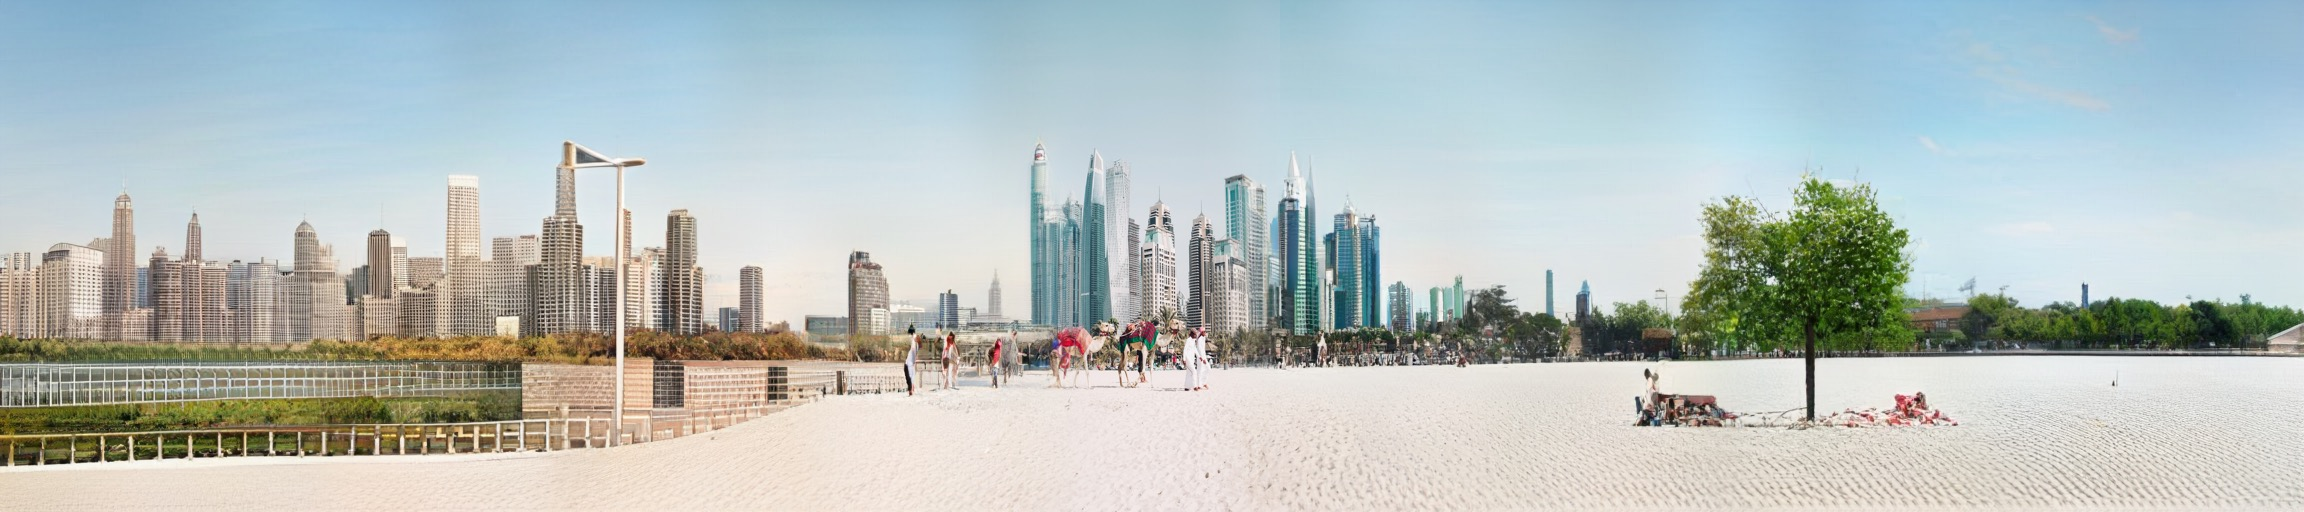
\includegraphics[ height=\tmpwidth]{figures/panorama/fredrik-ohlander-fCW1hWq2nq0-unsplash.jpg_input.jpeg} \\ 

% \includegraphics[ height=\tmpwidth]{figures/panorama/jairph-1XLyzi17Z2M-unsplash.jpg_input.jpeg} \\ 
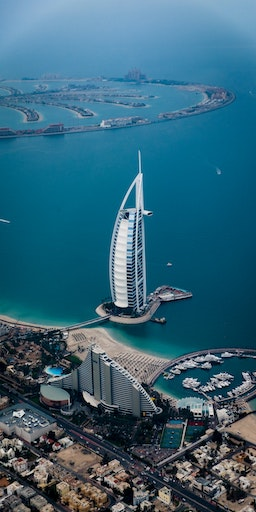
\includegraphics[ height=\tmpwidth]{figures/panorama/christoph-schulz-7tb-b37yHx4-unsplash.jpg} &
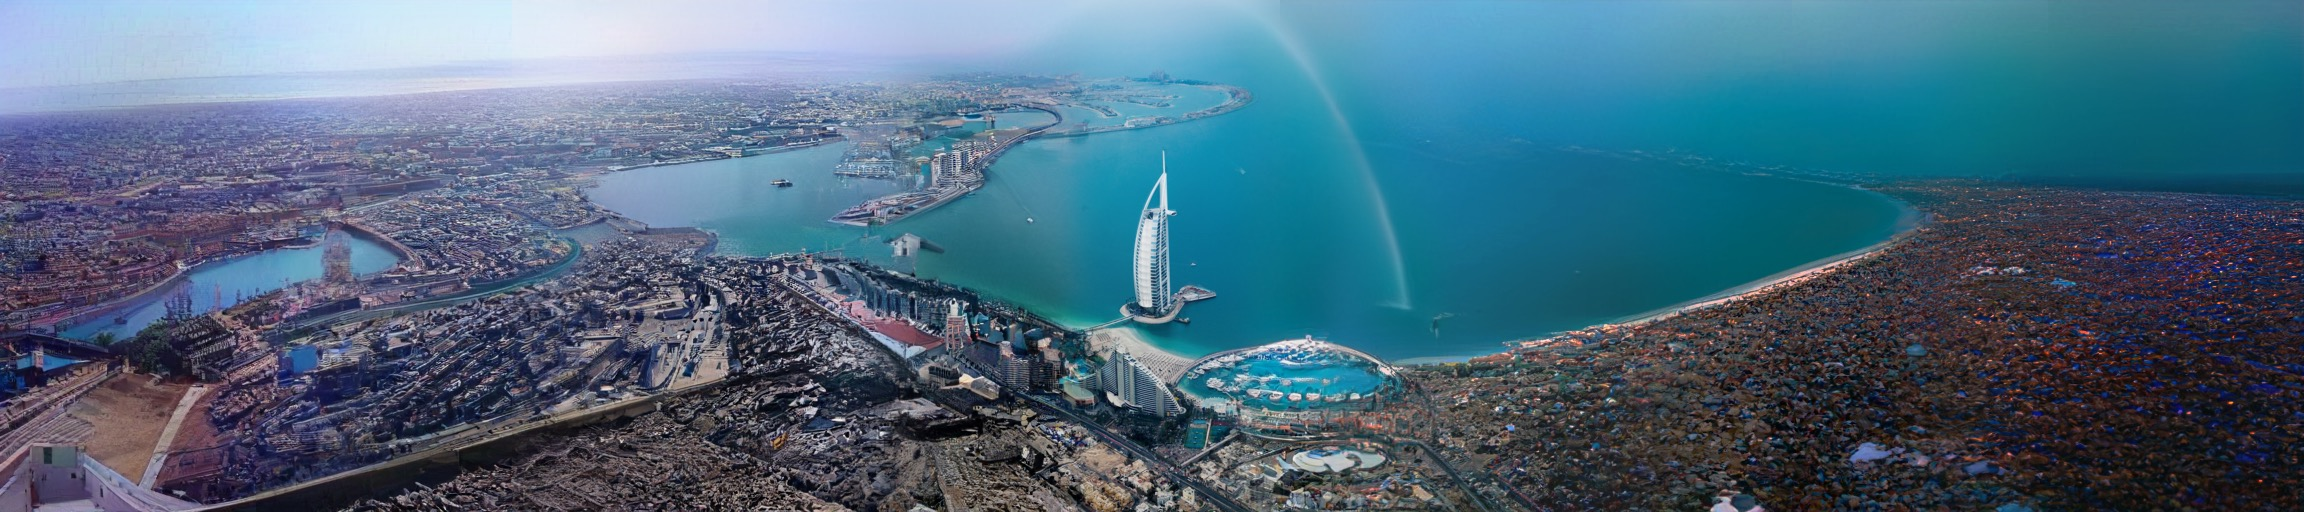
\includegraphics[ height=\tmpwidth]{figures/panorama/christoph-schulz-7tb-b37yHx4-unsplash.jpg_input.jpeg} \\ 
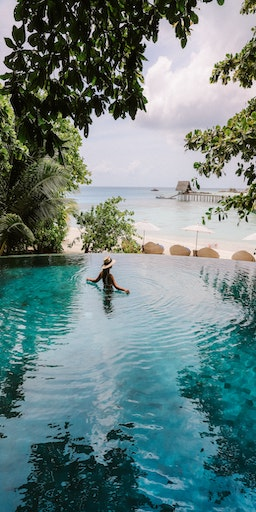
\includegraphics[ height=\tmpwidth]{figures/panorama/chelsea-gates-0653_wY0nRc-unsplash.jpg} &
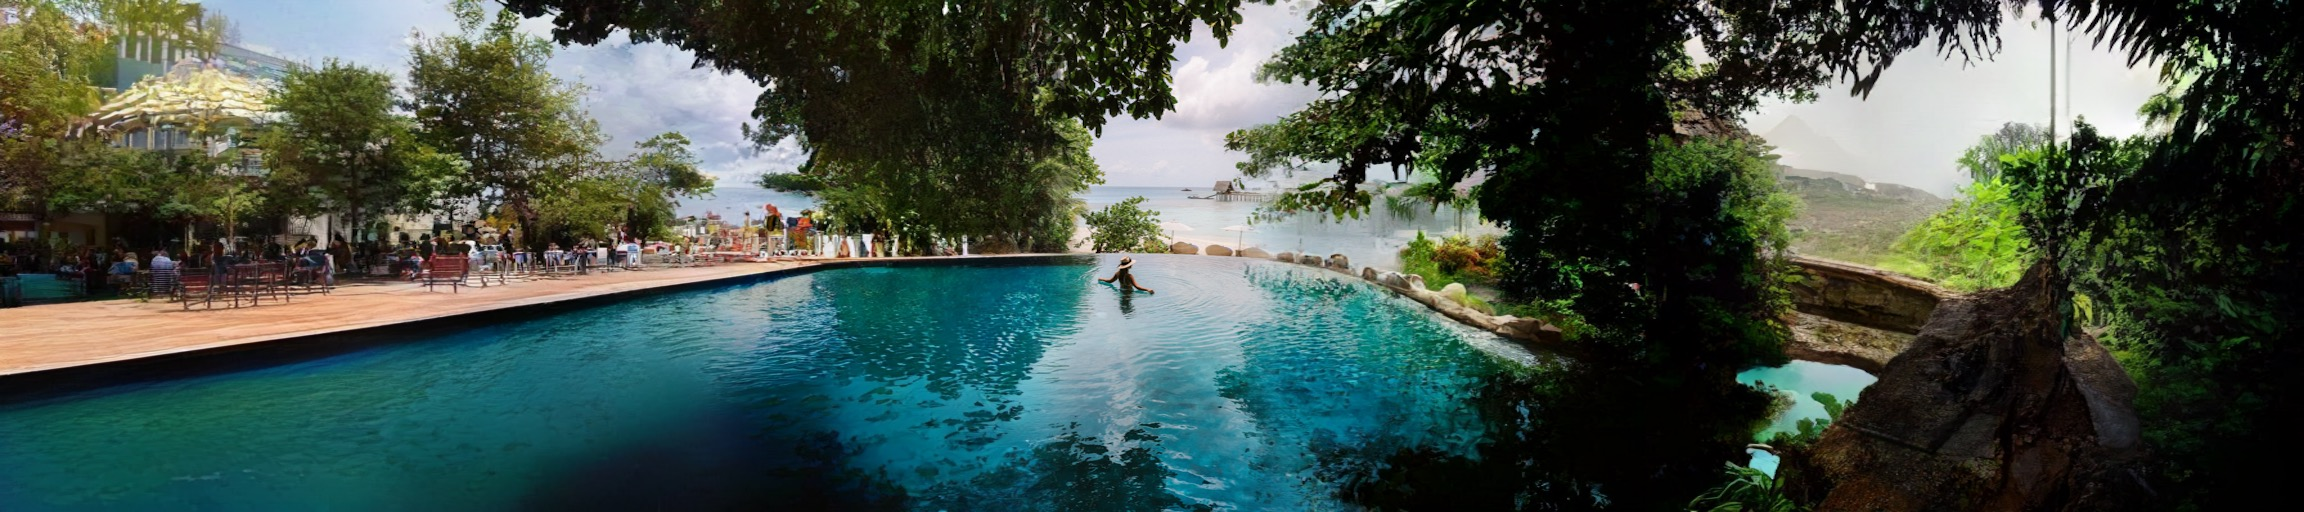
\includegraphics[ height=\tmpwidth]{figures/panorama/chelsea-gates-0653_wY0nRc-unsplash.jpg_input.jpeg} \\ 
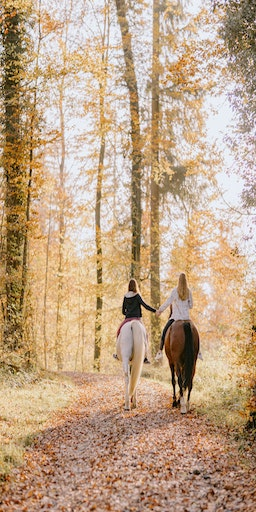
\includegraphics[ height=\tmpwidth]{figures/panorama/janosch-diggelmann-qXzNdOfGnbw-unsplash.jpg} &
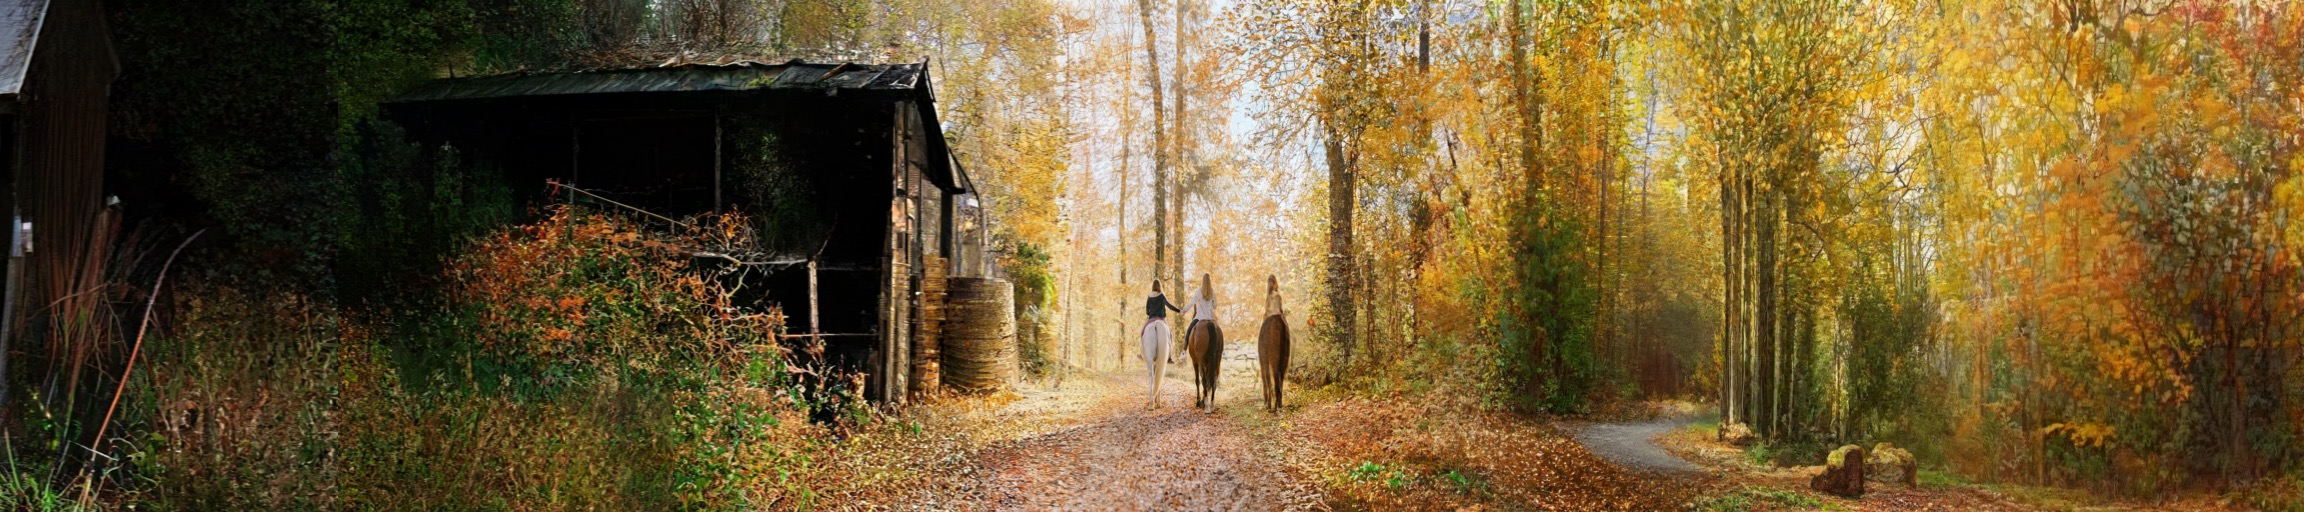
\includegraphics[ height=\tmpwidth]{figures/panorama/janosch-diggelmann-qXzNdOfGnbw-unsplash2.jpg_input.jpeg} \\ 

    \end{tabular}
    \vspace{-3mm}
    \caption{More Samples of Horizontal Image Extrapolation (from 512$\times$256 to 512$\times$2304). The synthesized "panoramas" are created by repeatedly applying \model's outpainting abilities horizontally in both directions.}
    %\vspace{-6mm}
    \label{fig:supp_panorama}
\end{figure*}



We show more examples of class-conditional image editing in Figure~\ref{fig:supp_editing}, and examples of image-conditional panorama synthesis in Figure~\ref{fig:supp_panorama}. 

\suppsection{Image Outpainting Comparisons with SOTA Transformer-based Approaches}
\label{sec:supp_outpainting_comparison_with_transformers}
In Figure~\ref{fig:supp_uncropgpt-1} and \ref{fig:supp_uncropgpt-2}, we show a few outpainting comparisons among \model, ImageGPT\cite{chen2020imagegpt}, and VQGAN\cite{Esser21vqgan}. In each set of images, we show the groundtruth (left), extrapolated samples using only the top half of the groundtruth (middle), and extrapolated samples using only the bottom half of the groundtruth (right). 

\model and VQGAN can both perform on higher resolutions by taking advantage of tokenization and thus achieve higher sample fidelity than ImageGPT, which runs on a maximum resolution of $192\times192$. At the same time, \model demonstrates stronger flexibility than ImageGPT and VQGAN in that it can outpaint in arbitrary directions (\eg both upward and downward), while ImageGPT and VQGAN can only handle outpainting in one direction with a single model due to their autoregressive natures.

\renewcommand{\tmpwidth}{22mm}
\setlength{\tabcolsep}{2pt}
\begin{figure*}[!ht]
    \centering
    \begin{tabular}{cc cccc ccc}
% \multirow{5}{*}{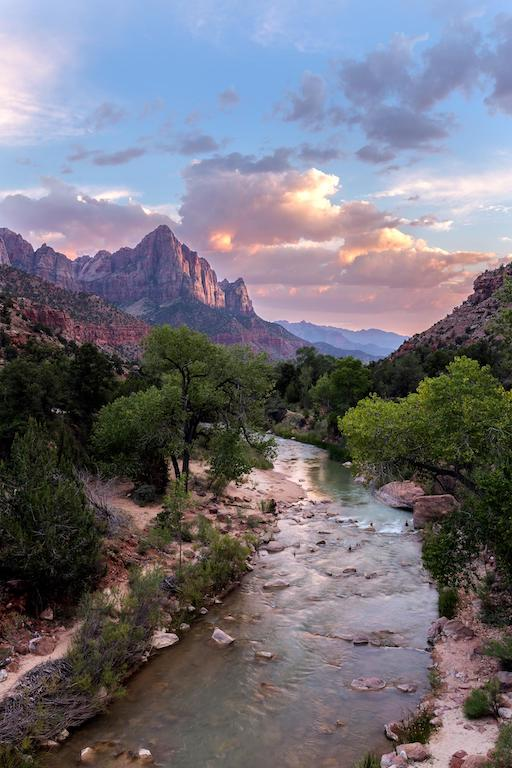
\includegraphics[width=\tmpwidth]{figures/supp_uncropgpt/1_input.jpg}}
\toprule
Groundtruth  & 
 &\multicolumn{3}{c}{ ------ Outpaint bottom 50\% ------ } & &\multicolumn{3}{c}{ ------ Outpaint top 50\% ------ }  
\\
& 
 \raisebox{0.85\tmpwidth }{\rotatebox[origin=l]{90}{ ImageGPT\cite{chen2020imagegpt}}} & 


\includegraphics[width=\tmpwidth]{figures/supp_uncropgpt/3_gpt1.jpg}&
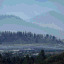
\includegraphics[width=\tmpwidth]{figures/supp_uncropgpt/3_gpt2.jpg}&
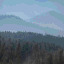
\includegraphics[width=\tmpwidth]{figures/supp_uncropgpt/3_gpt3.jpg} &
\\

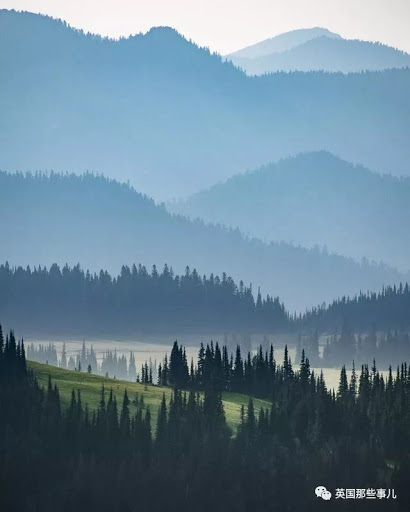
\includegraphics[width=\tmpwidth]{figures/supp_uncropgpt/3_input.jpg} &
 \raisebox{0.85\tmpwidth }{\rotatebox[origin=l]{90}{ VQGAN\cite{Esser21vqgan}}} & 

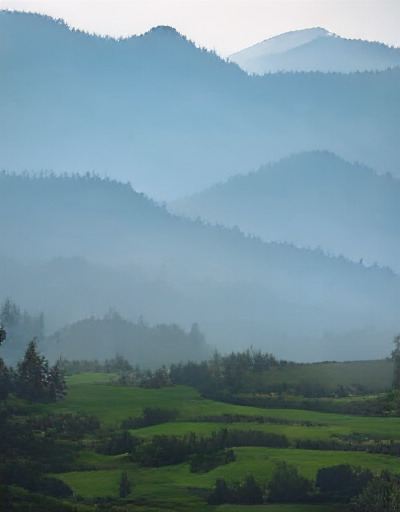
\includegraphics[width=\tmpwidth]{figures/supp_uncropgpt/3_taming1.jpg}&
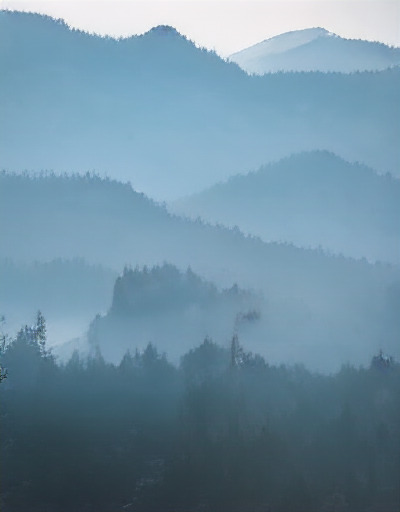
\includegraphics[width=\tmpwidth]{figures/supp_uncropgpt/3_taming2.jpg}&
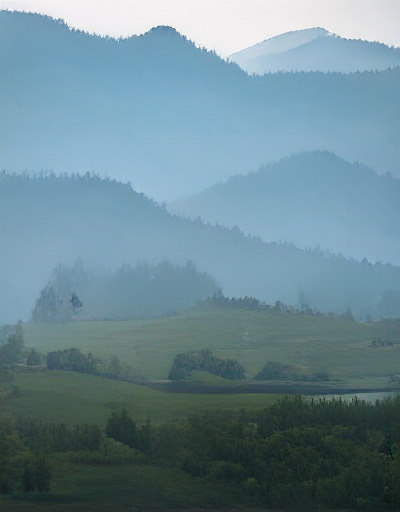
\includegraphics[width=\tmpwidth]{figures/supp_uncropgpt/3_taming3.jpg} &
\\
& 
 \raisebox{0.85\tmpwidth }{\rotatebox[origin=l]{90}{\model (Ours)}} & 
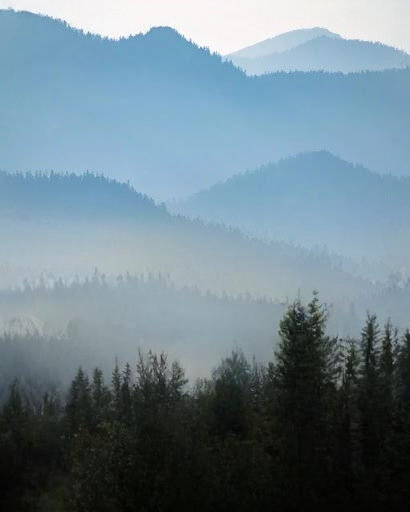
\includegraphics[width=\tmpwidth]{figures/supp_uncropgpt/3_ours13.jpeg}&
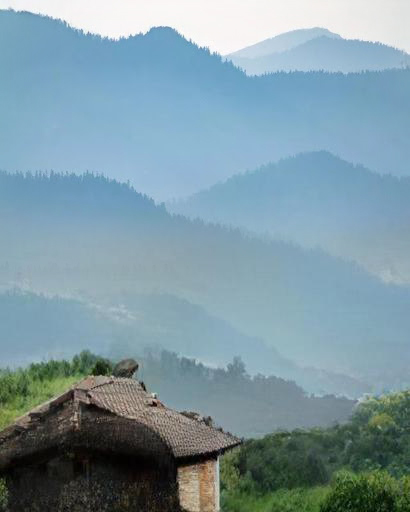
\includegraphics[width=\tmpwidth]{figures/supp_uncropgpt/3_ours23.jpeg}&
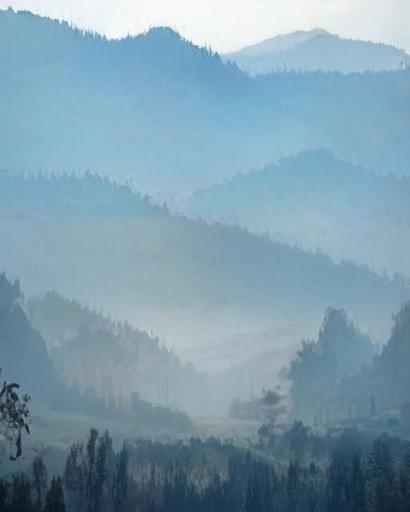
\includegraphics[width=\tmpwidth]{figures/supp_uncropgpt/3_ours20.jpeg} &
&
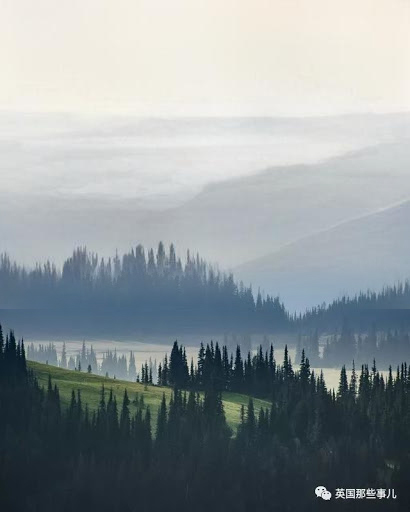
\includegraphics[width=\tmpwidth]{figures/supp_uncropgpt/3_top_ours7.jpeg}&
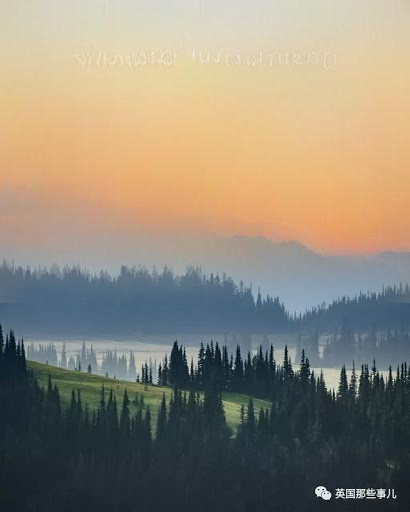
\includegraphics[width=\tmpwidth]{figures/supp_uncropgpt/3_top_ours2.jpeg}&
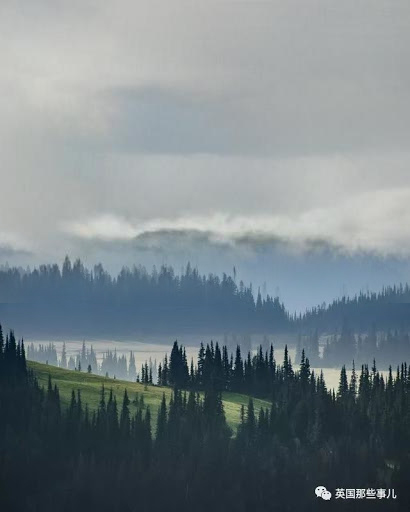
\includegraphics[width=\tmpwidth]{figures/supp_uncropgpt/3_top_ours1.jpeg}

% &\multicolumn{3}{c}{--- MaskGIT's Samples (Outpainting Bottom Half) ---} &\multicolumn{3}{c}{--- MaskGIT's Samples (Outpainting Top Half) ---}  
\\
& 
 \raisebox{0.85\tmpwidth }{\rotatebox[origin=l]{90}{ ImageGPT\cite{chen2020imagegpt}}} & 


\includegraphics[width=\tmpwidth]{figures/supp_uncropgpt/4_gpt1.jpg}&
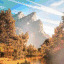
\includegraphics[width=\tmpwidth]{figures/supp_uncropgpt/4_gpt2.jpg}&
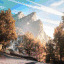
\includegraphics[width=\tmpwidth]{figures/supp_uncropgpt/4_gpt3.jpg} &
\\
% & \multicolumn{3}{c}{------ ImageGPT\cite{chen2020imagegpt}'s Samples ------}  &
% \\
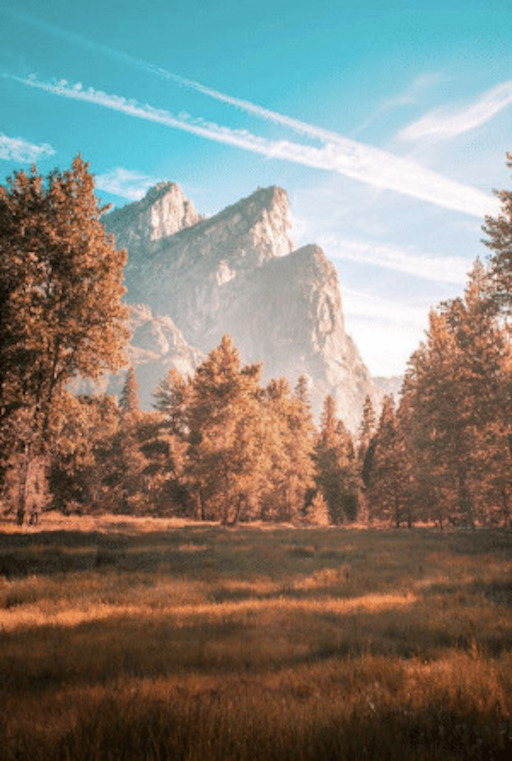
\includegraphics[width=\tmpwidth]{figures/supp_uncropgpt/4_input.jpg} &
 \raisebox{0.85\tmpwidth }{\rotatebox[origin=l]{90}{VQGAN\cite{Esser21vqgan}}} & 
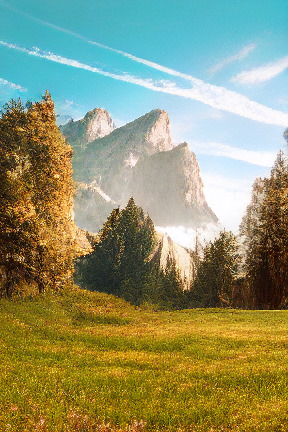
\includegraphics[width=\tmpwidth]{figures/supp_uncropgpt/4_taming1.jpg}&
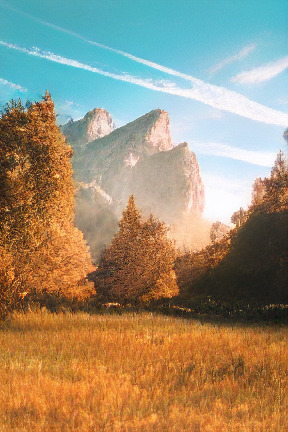
\includegraphics[width=\tmpwidth]{figures/supp_uncropgpt/4_taming2.jpg}&
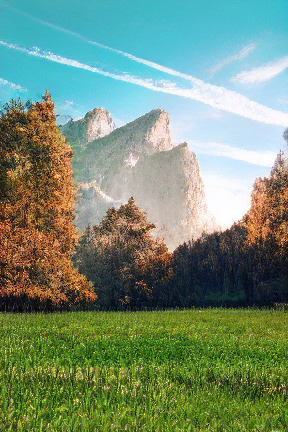
\includegraphics[width=\tmpwidth]{figures/supp_uncropgpt/4_taming3.jpg} &
\\
& 
 \raisebox{0.85\tmpwidth }{\rotatebox[origin=l]{90}{\model (Ours)}} & 
 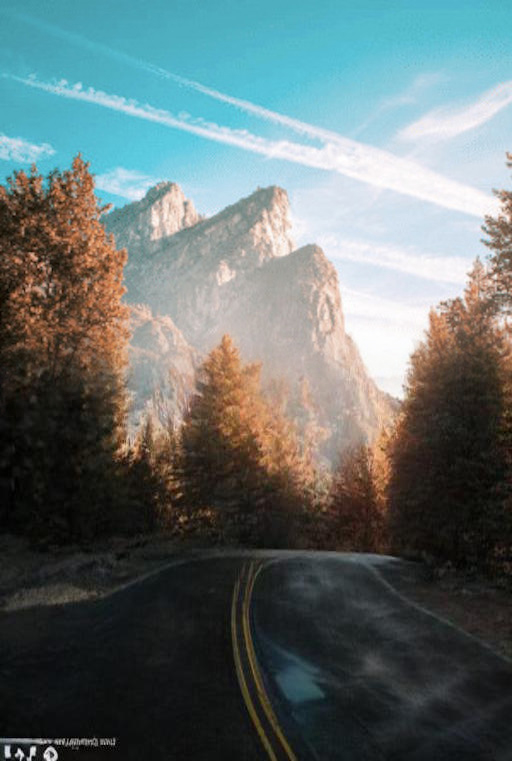
\includegraphics[width=\tmpwidth]{figures/supp_uncropgpt/4_ours1.jpeg}&
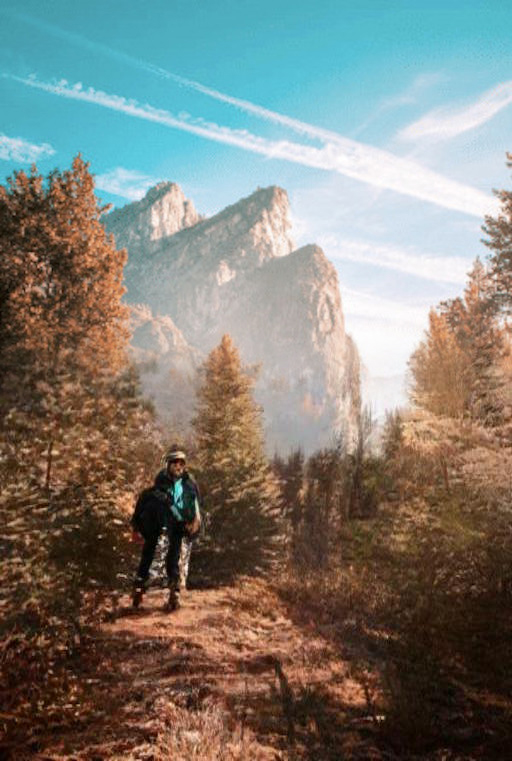
\includegraphics[width=\tmpwidth]{figures/supp_uncropgpt/4_ours13.jpeg}&
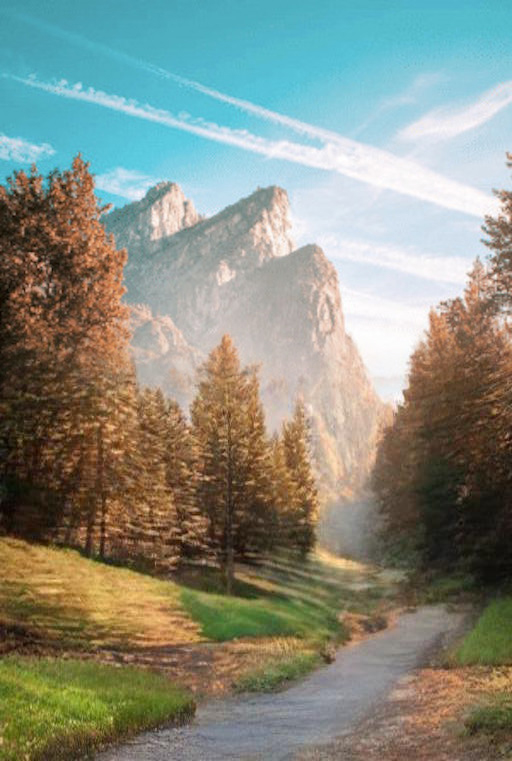
\includegraphics[width=\tmpwidth]{figures/supp_uncropgpt/4_ours27.jpeg} &
&
 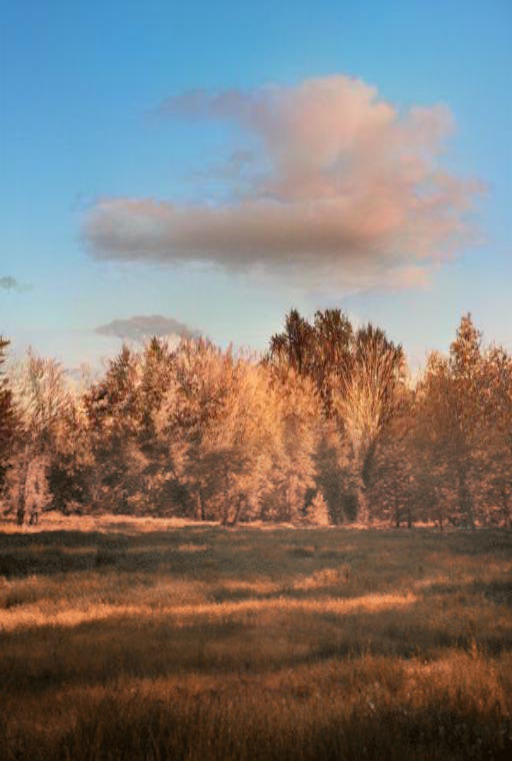
\includegraphics[width=\tmpwidth]{figures/supp_uncropgpt/4_top_ours7.jpeg}&
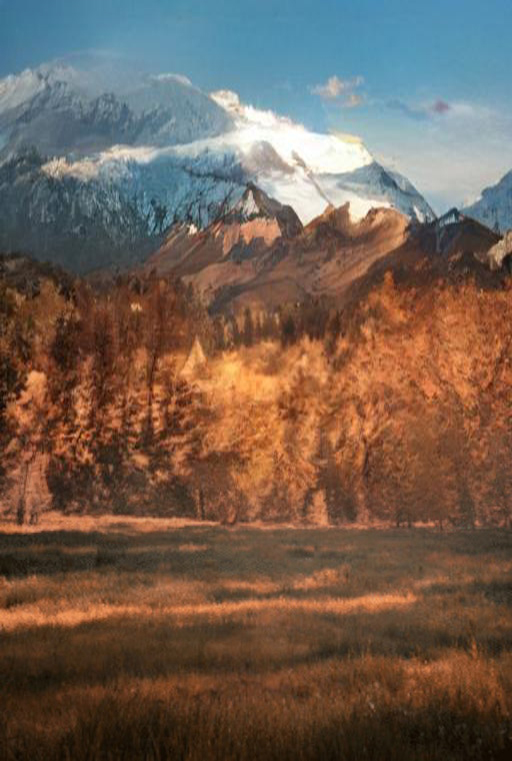
\includegraphics[width=\tmpwidth]{figures/supp_uncropgpt/4_top_ours3.jpeg}&
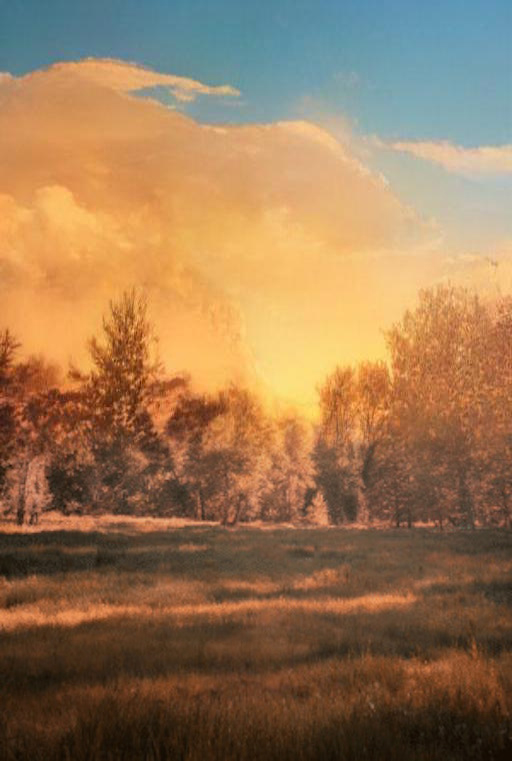
\includegraphics[width=\tmpwidth]{figures/supp_uncropgpt/4_top_ours6.jpeg}
\\
      
    \end{tabular}
    \vspace{-2mm}
    \caption{与基于像素的方法ImageGPT和基于Transformer的方法VQGAN的外推比较。
    }
    % \vspace{-10mm}
    \label{fig:supp_uncropgpt-1}
\end{figure*}


% \begin{figure*}[!ht]
%     \centering
%     \begin{tabular}{cc ccc ccc}
% &
% 
\includegraphics[width=\tmpwidth]{figures/supp_uncropgpt/1_gpt1.jpg}&
% 
\includegraphics[width=\tmpwidth]{figures/supp_uncropgpt/1_gpt2.jpg}&
% 
\includegraphics[width=\tmpwidth]{figures/supp_uncropgpt/1_gpt3.jpg}&
% \\
% & \multicolumn{3}{c}{------ ImageGPT\cite{chen2020imagegpt}'s Samples ------}  &
% \\

% 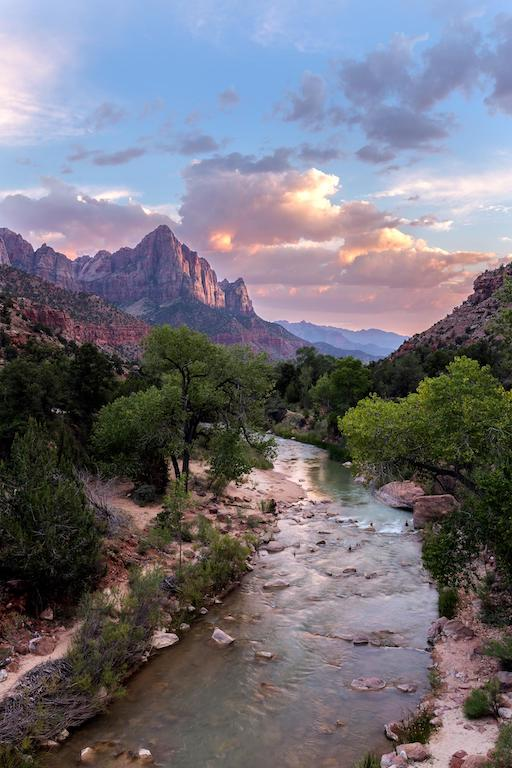
\includegraphics[width=\tmpwidth]{figures/supp_uncropgpt/1_input.jpg} &
% 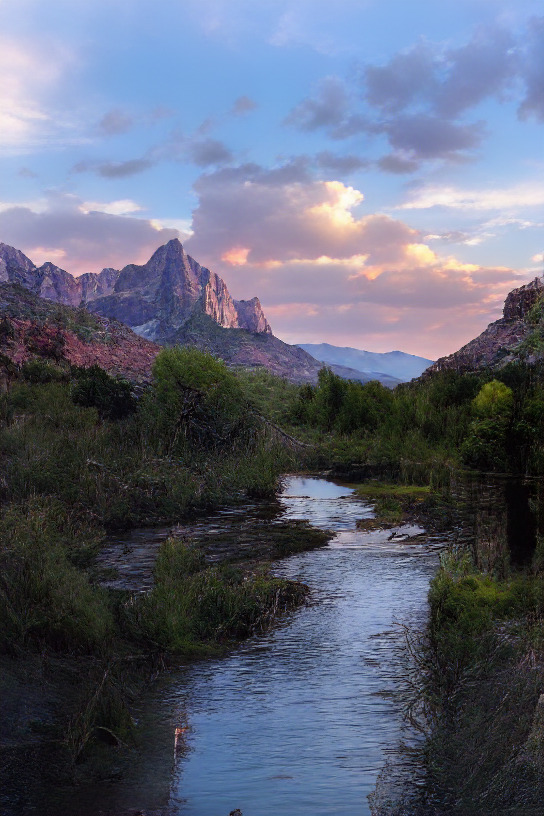
\includegraphics[width=\tmpwidth]{figures/supp_uncropgpt/1_taming1.jpg}&
% 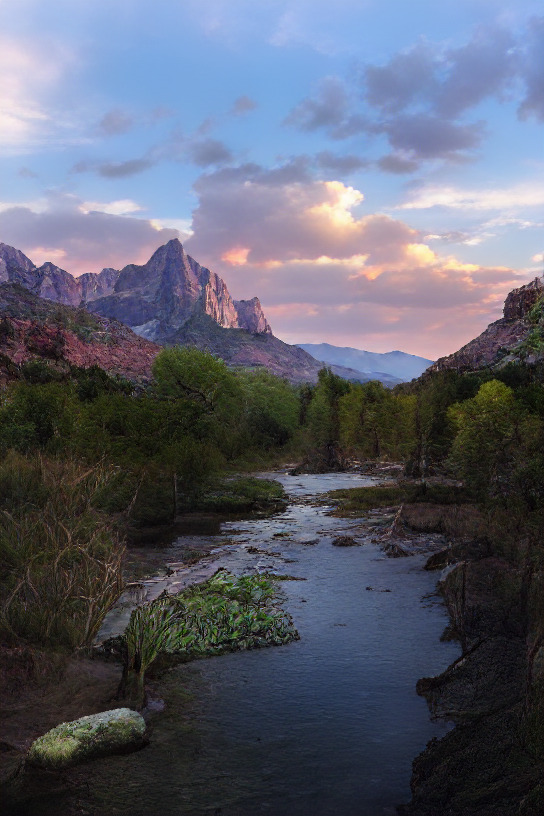
\includegraphics[width=\tmpwidth]{figures/supp_uncropgpt/1_taming2.jpg}&
% 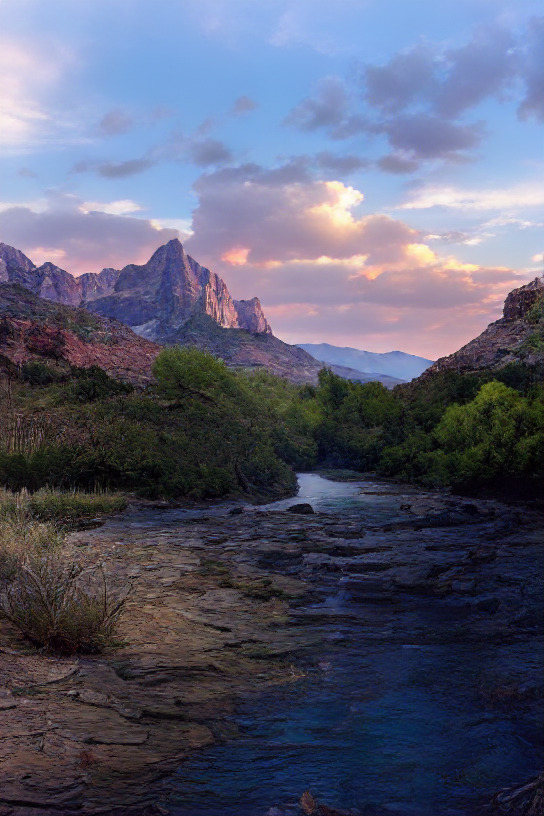
\includegraphics[width=\tmpwidth]{figures/supp_uncropgpt/1_taming3.jpg} &
% \\
% Groundtruth  & \multicolumn{3}{c}{------ VQGAN\cite{Esser21vqgan}'s Samples ------}  &
% \\
% % Groundtruth  & \multicolumn{3}{c}{------ VQGAN\cite{Esser21vqgan}'s Samples ------}  &
% % Groundtruth  & \multicolumn{3}{c}{------ VQGAN\cite{Esser21vqgan}'s Samples ------}  
  
% &
% 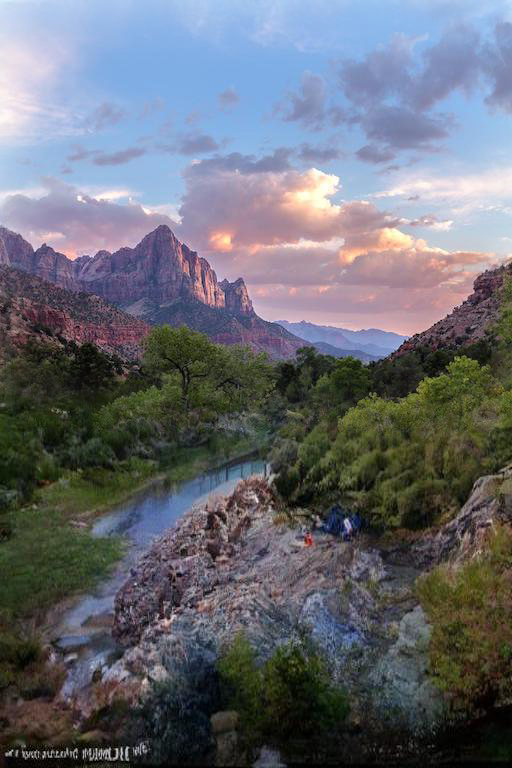
\includegraphics[width=\tmpwidth]{figures/supp_uncropgpt/1_ours26.jpeg}&
% 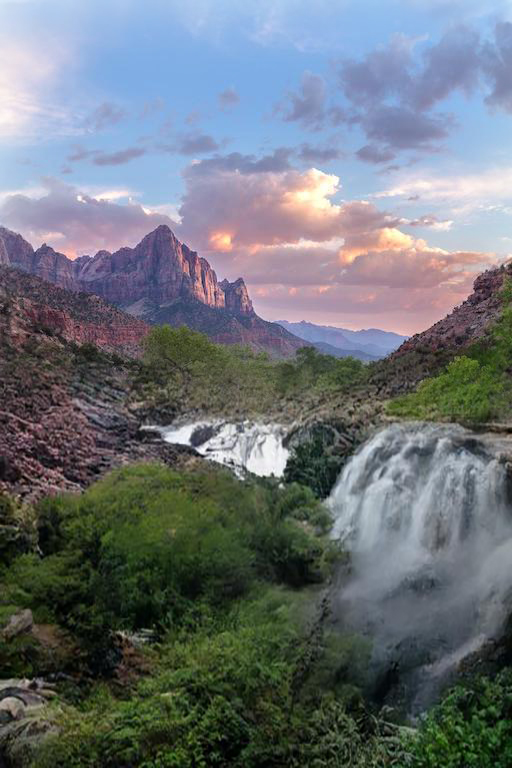
\includegraphics[width=\tmpwidth]{figures/supp_uncropgpt/1_ours5.jpeg}&
% 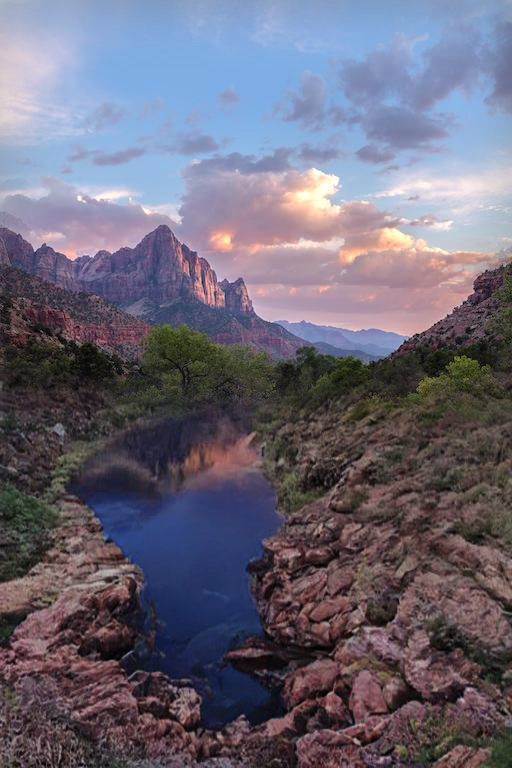
\includegraphics[width=\tmpwidth]{figures/supp_uncropgpt/1_ours8.jpeg} &
% 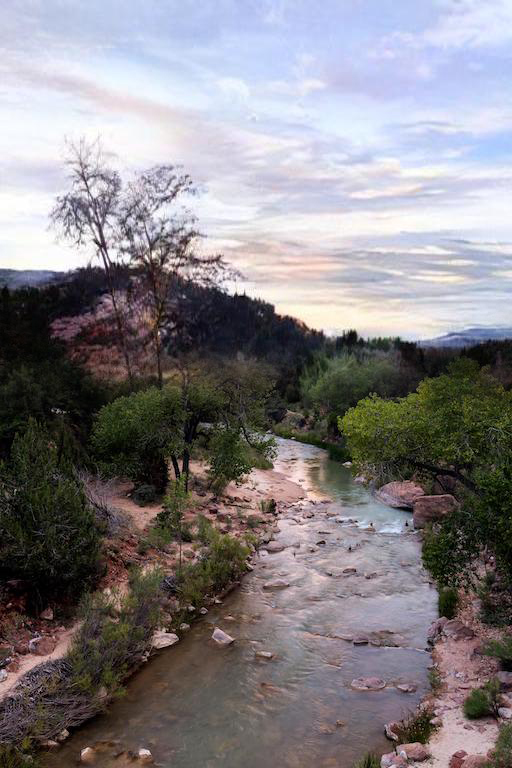
\includegraphics[width=\tmpwidth]{figures/supp_uncropgpt/1_top_ours1.jpeg}&
% 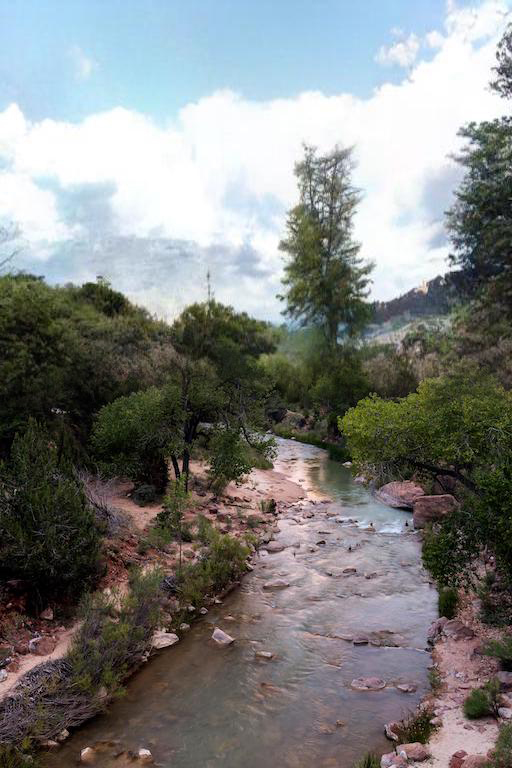
\includegraphics[width=\tmpwidth]{figures/supp_uncropgpt/1_top_ours7.jpeg}&
% 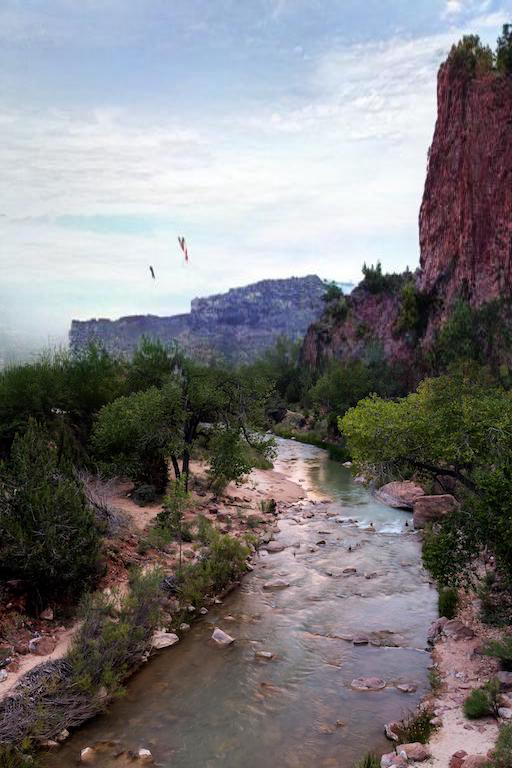
\includegraphics[width=\tmpwidth]{figures/supp_uncropgpt/1_top_ours8.jpeg} &

% \\
%  &\multicolumn{3}{c}{--- MaskGIT's Samples (Outpainting Bottom Half) ---} &\multicolumn{3}{c}{--- MaskGIT's Samples (Outpainting Top Half) ---}  
% \\ 
% \\

% &
% 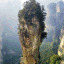
\includegraphics[width=\tmpwidth]{figures/supp_uncropgpt/2_gpt1.jpg}&
% 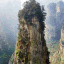
\includegraphics[width=\tmpwidth]{figures/supp_uncropgpt/2_gpt2.jpg}&
% 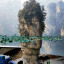
\includegraphics[width=\tmpwidth]{figures/supp_uncropgpt/2_gpt3.jpg} &
% \\
% & \multicolumn{3}{c}{------ ImageGPT\cite{chen2020imagegpt}'s Samples ------}  &
% \\

% 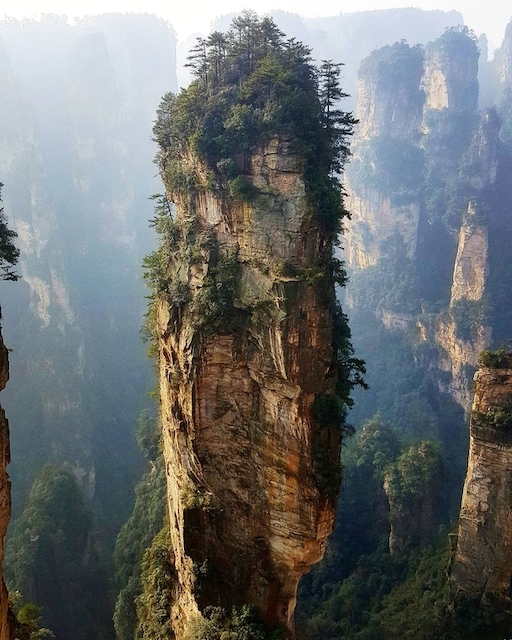
\includegraphics[width=\tmpwidth]{figures/supp_uncropgpt/2_input.jpg} &
% 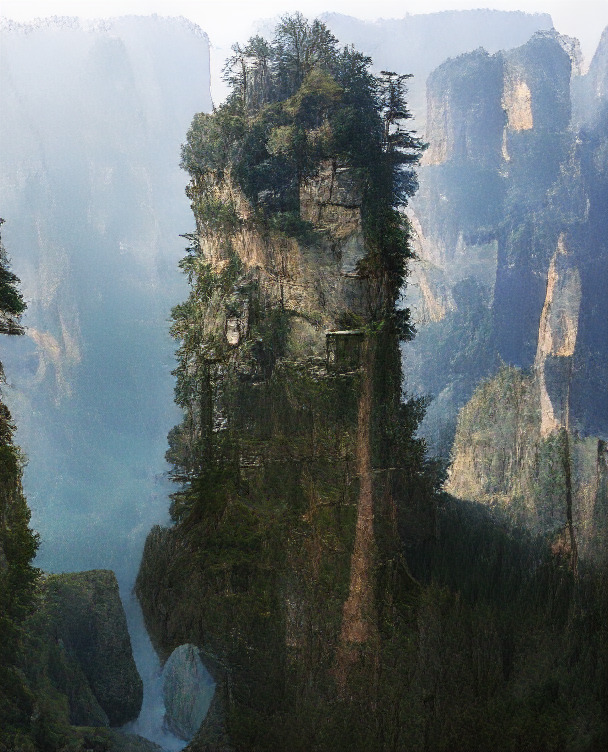
\includegraphics[width=\tmpwidth]{figures/supp_uncropgpt/2_taming1.jpg}&
% 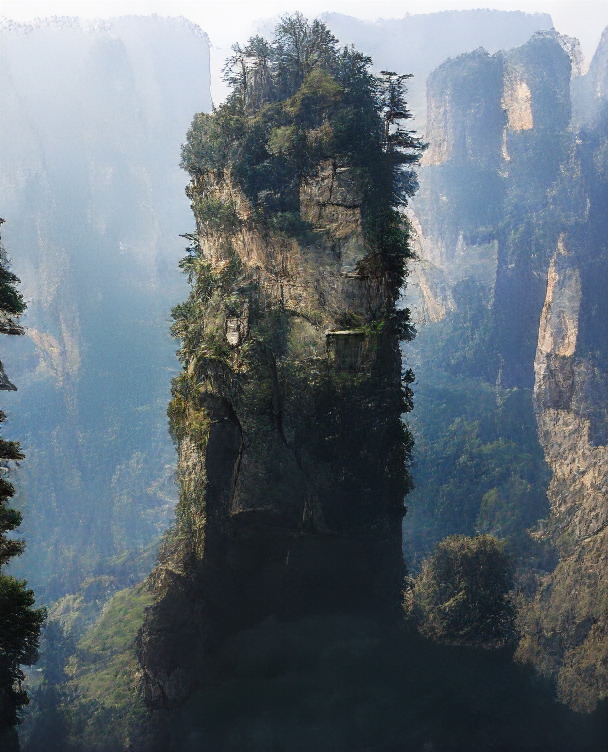
\includegraphics[width=\tmpwidth]{figures/supp_uncropgpt/2_taming2.jpg}&
% 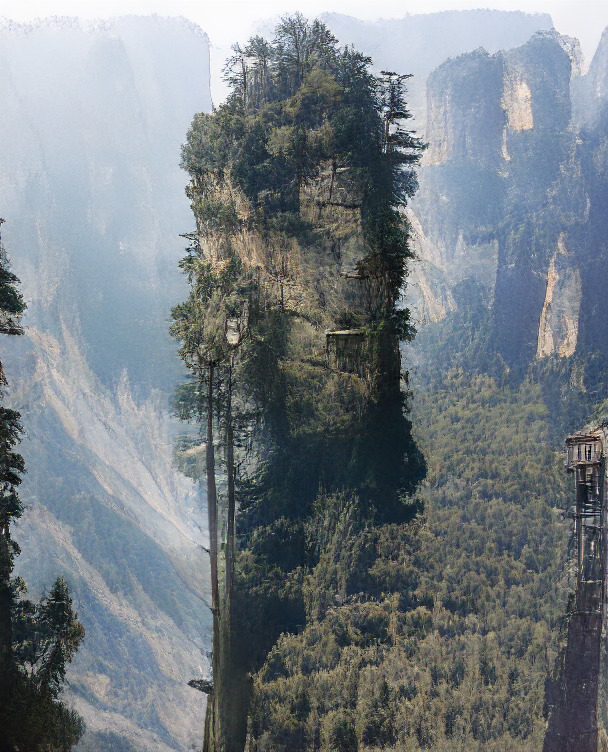
\includegraphics[width=\tmpwidth]{figures/supp_uncropgpt/2_taming3.jpg} &
%  \\   

% Groundtruth  & \multicolumn{3}{c}{------ VQGAN\cite{Esser21vqgan}'s Samples ------}  &
% \\
% &
% 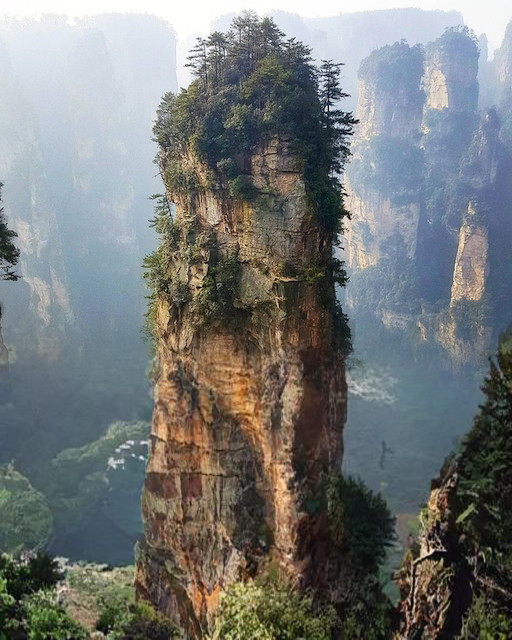
\includegraphics[width=\tmpwidth]{figures/supp_uncropgpt/2_ours4.jpeg}&
% 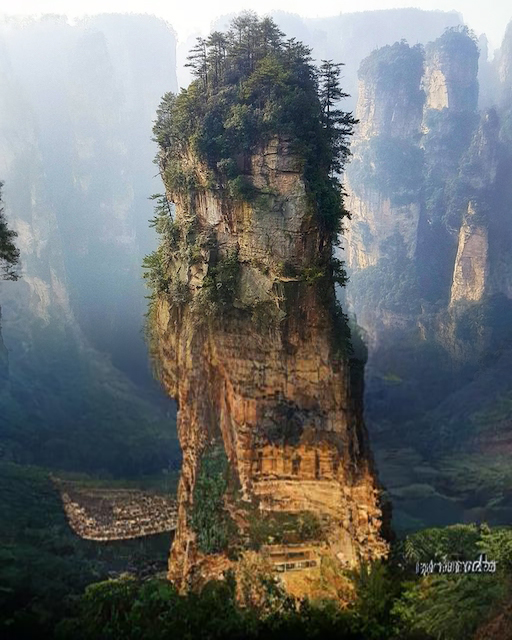
\includegraphics[width=\tmpwidth]{figures/supp_uncropgpt/2_ours11.jpeg}&
% 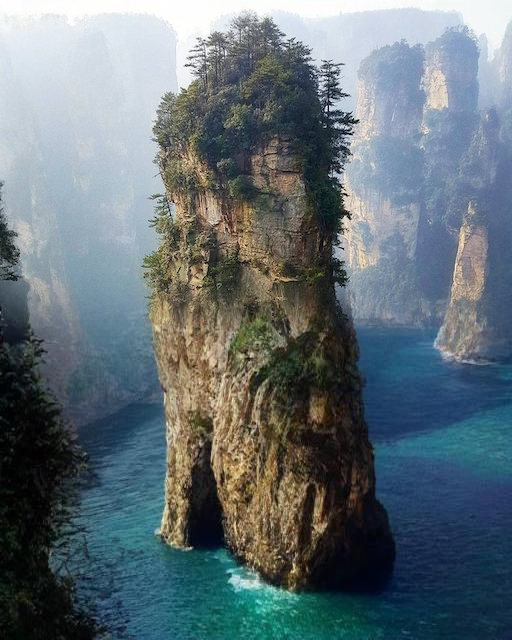
\includegraphics[width=\tmpwidth]{figures/supp_uncropgpt/2_ours19.jpeg} &
% 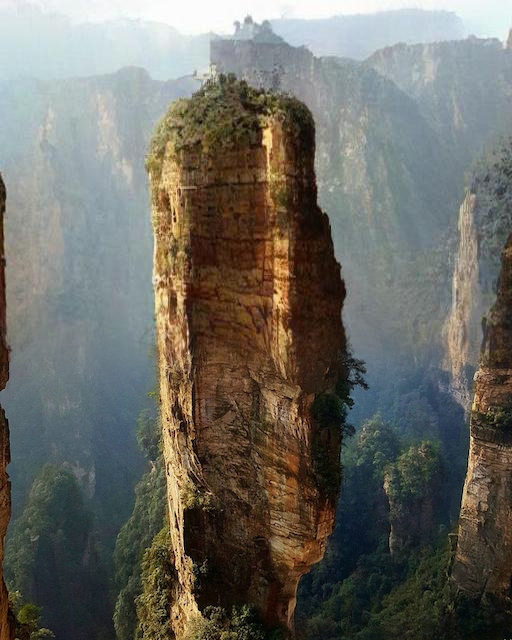
\includegraphics[width=\tmpwidth]{figures/supp_uncropgpt/2_top_ours3.jpeg}&
% 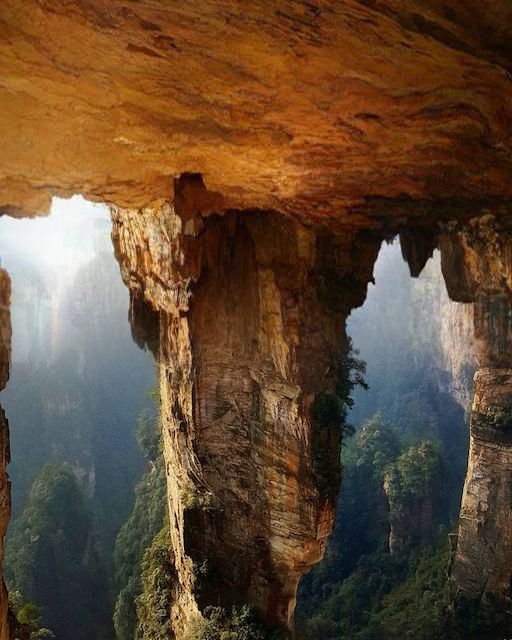
\includegraphics[width=\tmpwidth]{figures/supp_uncropgpt/2_top_ours2.jpeg}&
% 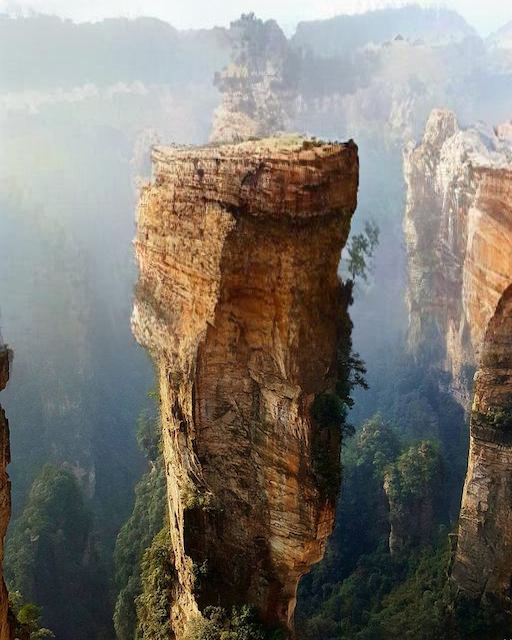
\includegraphics[width=\tmpwidth]{figures/supp_uncropgpt/2_top_ours5.jpeg} &


% \\
% &\multicolumn{3}{c}{--- MaskGIT's Samples (Outpainting Bottom Half) ---} &\multicolumn{3}{c}{--- MaskGIT's Samples (Outpainting Top Half) ---}  
% \\ 
       
%     \end{tabular}
%     \caption{Comparing our approach with the pixel-based approach ImageGPT\cite{chen2020imagegpt} and the transformer-based approach VQGAN\cite{Esser21vqgan}.
%     }
%     \vspace{-6mm}
%     \label{fig:supp_uncropgpt-2}
% \end{figure*}




\renewcommand{\tmpwidth}{22mm}
\setlength{\tabcolsep}{2pt}
\begin{figure*}[!ht]
    \centering
    \begin{tabular}{cc cccc ccc}
\toprule
Groundtruth  & 
 &\multicolumn{3}{c}{ ------ Outpaint bottom 50\% ------ } & &\multicolumn{3}{c}{ ------ Outpaint top 50\% ------ }  
\\
& 
 \raisebox{0.85\tmpwidth }{\rotatebox[origin=l]{90}{ ImageGPT\cite{chen2020imagegpt}}} & 


\includegraphics[width=\tmpwidth]{figures/supp_uncropgpt/1_gpt1.jpg}&

\includegraphics[width=\tmpwidth]{figures/supp_uncropgpt/1_gpt2.jpg}&

\includegraphics[width=\tmpwidth]{figures/supp_uncropgpt/1_gpt3.jpg}&
% \\
% & \multicolumn{3}{c}{------ ImageGPT\cite{chen2020imagegpt}'s Samples ------}  &
\\
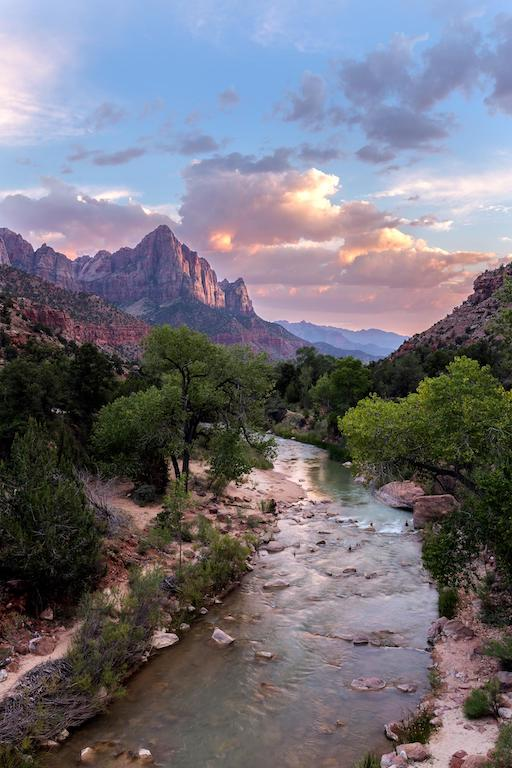
\includegraphics[width=\tmpwidth]{figures/supp_uncropgpt/1_input.jpg} &
 \raisebox{0.85\tmpwidth }{\rotatebox[origin=l]{90}{ VQGAN\cite{Esser21vqgan}}} & 
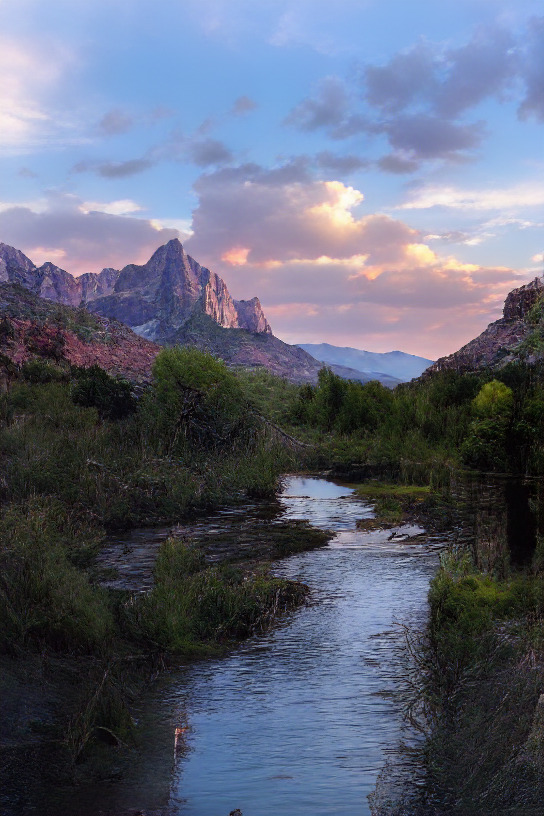
\includegraphics[width=\tmpwidth]{figures/supp_uncropgpt/1_taming1.jpg}&
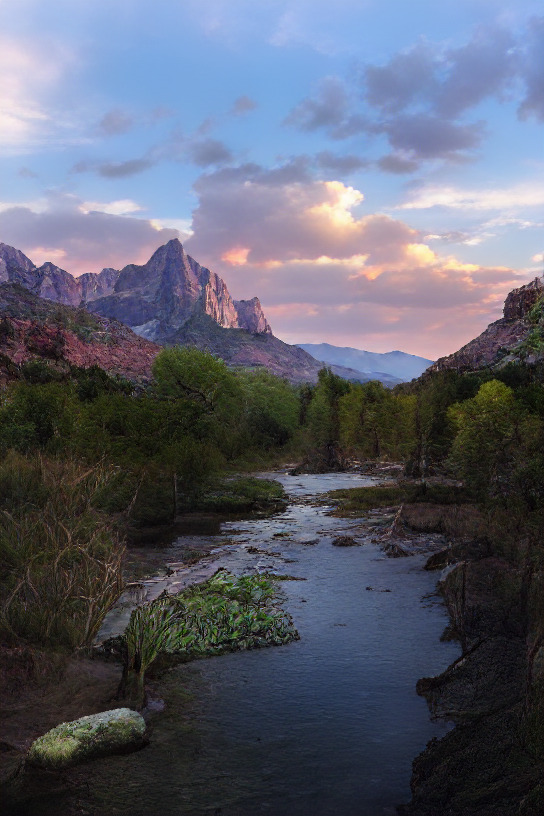
\includegraphics[width=\tmpwidth]{figures/supp_uncropgpt/1_taming2.jpg}&
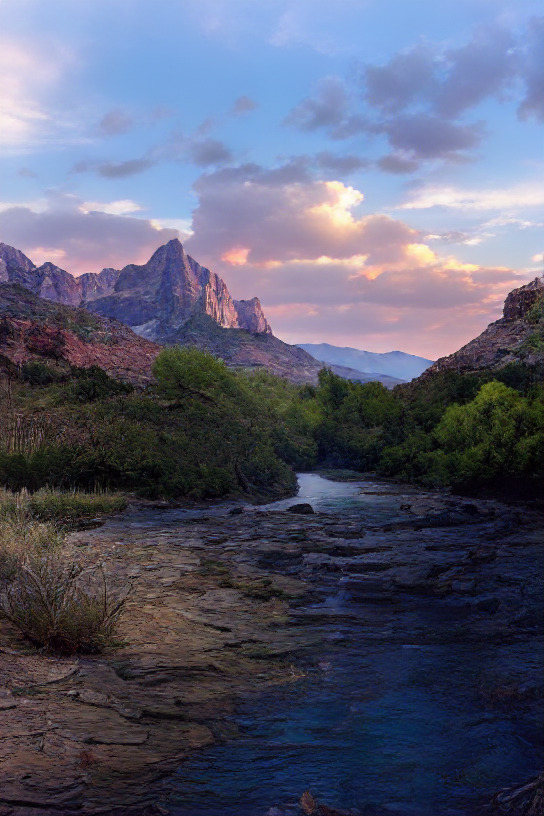
\includegraphics[width=\tmpwidth]{figures/supp_uncropgpt/1_taming3.jpg} &
\\
% Groundtruth  & \multicolumn{3}{c}{------ VQGAN\cite{Esser21vqgan}'s Samples ------}  &
% \\
% Groundtruth  & \multicolumn{3}{c}{------ VQGAN\cite{Esser21vqgan}'s Samples ------}  &
% Groundtruth  & \multicolumn{3}{c}{------ VQGAN\cite{Esser21vqgan}'s Samples ------}  
& 
 \raisebox{0.85\tmpwidth }{\rotatebox[origin=l]{90}{\model (Ours)}} & 
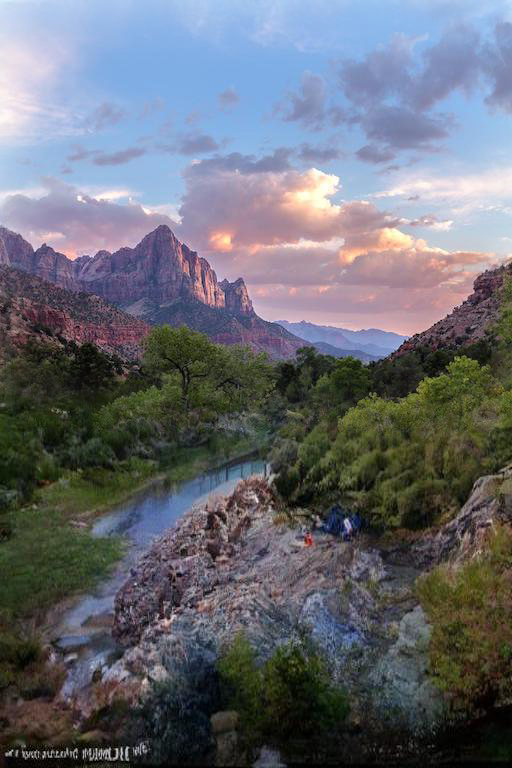
\includegraphics[width=\tmpwidth]{figures/supp_uncropgpt/1_ours26.jpeg}&
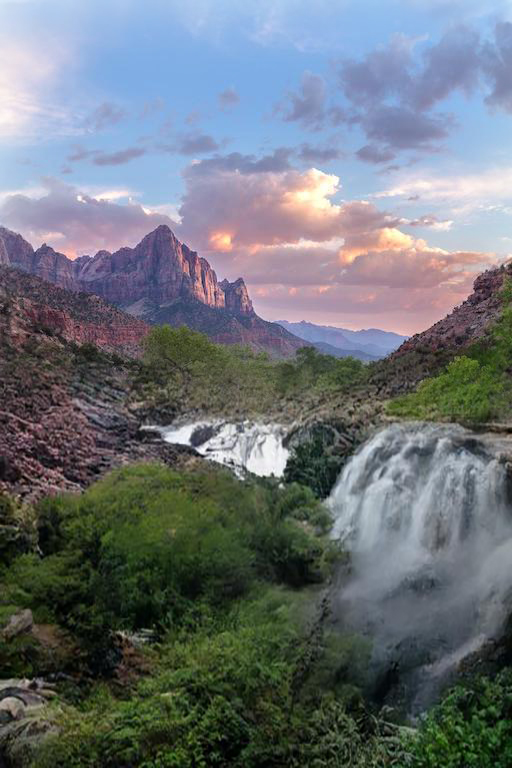
\includegraphics[width=\tmpwidth]{figures/supp_uncropgpt/1_ours5.jpeg}&
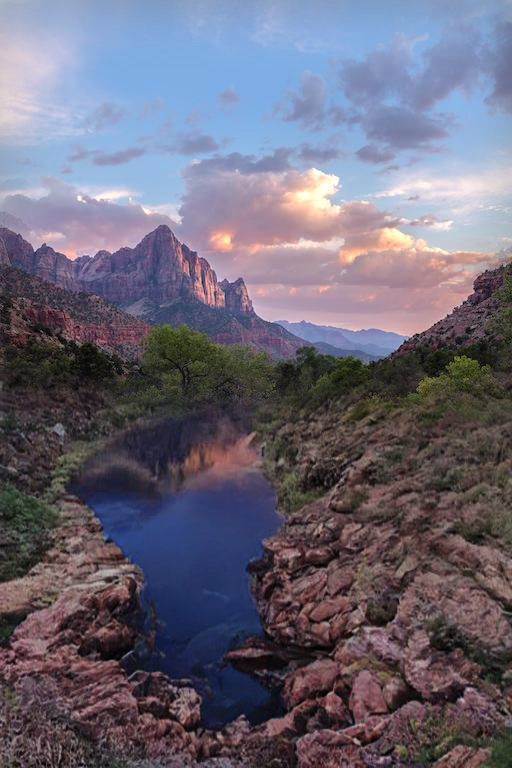
\includegraphics[width=\tmpwidth]{figures/supp_uncropgpt/1_ours8.jpeg} &
&
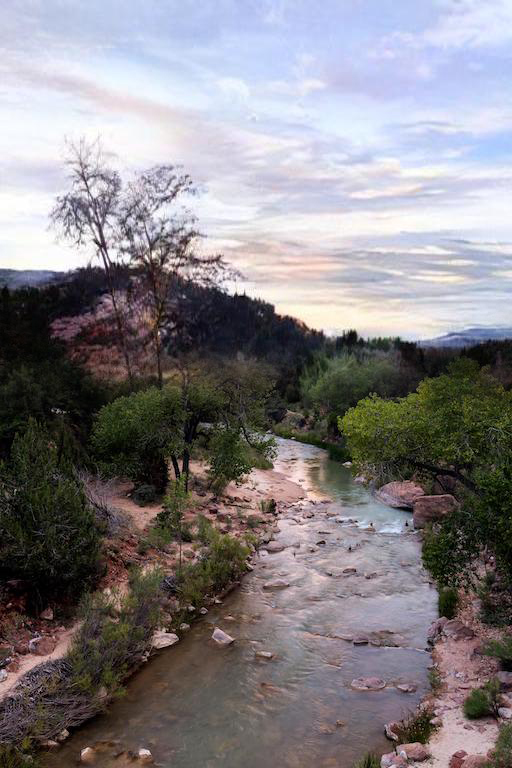
\includegraphics[width=\tmpwidth]{figures/supp_uncropgpt/1_top_ours1.jpeg}&
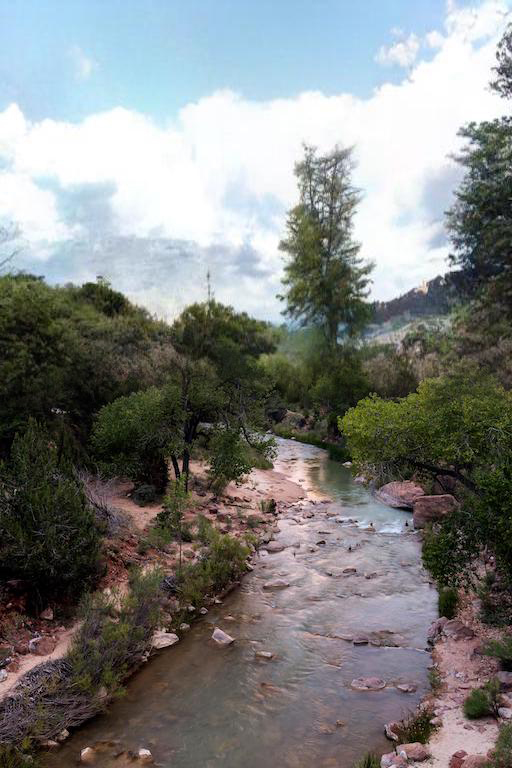
\includegraphics[width=\tmpwidth]{figures/supp_uncropgpt/1_top_ours7.jpeg}&
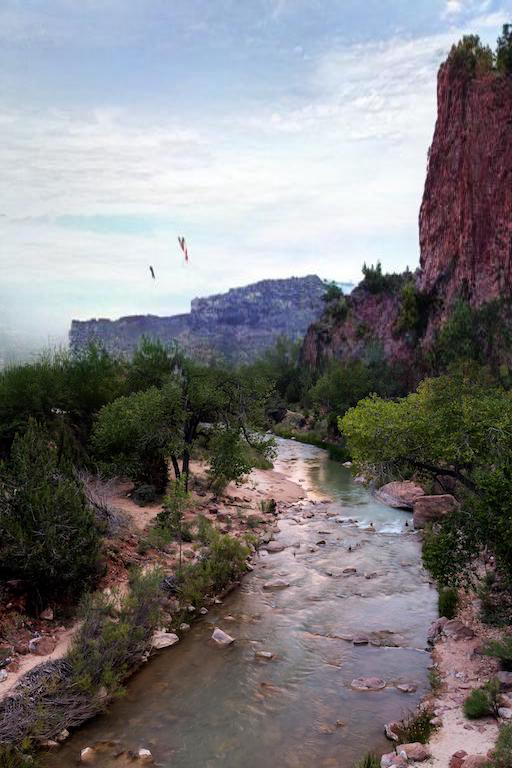
\includegraphics[width=\tmpwidth]{figures/supp_uncropgpt/1_top_ours8.jpeg}

\\
%  &\multicolumn{3}{c}{--- MaskGIT's Samples (Outpainting Bottom Half) ---} &\multicolumn{3}{c}{--- MaskGIT's Samples (Outpainting Top Half) ---}  
& 
 \raisebox{0.85\tmpwidth }{\rotatebox[origin=l]{90}{ ImageGPT\cite{chen2020imagegpt}}} & 
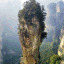
\includegraphics[width=\tmpwidth]{figures/supp_uncropgpt/2_gpt1.jpg}&
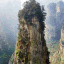
\includegraphics[width=\tmpwidth]{figures/supp_uncropgpt/2_gpt2.jpg}&
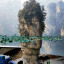
\includegraphics[width=\tmpwidth]{figures/supp_uncropgpt/2_gpt3.jpg} &
\\
% & \multicolumn{3}{c}{------ ImageGPT\cite{chen2020imagegpt}'s Samples ------}  &
% \\
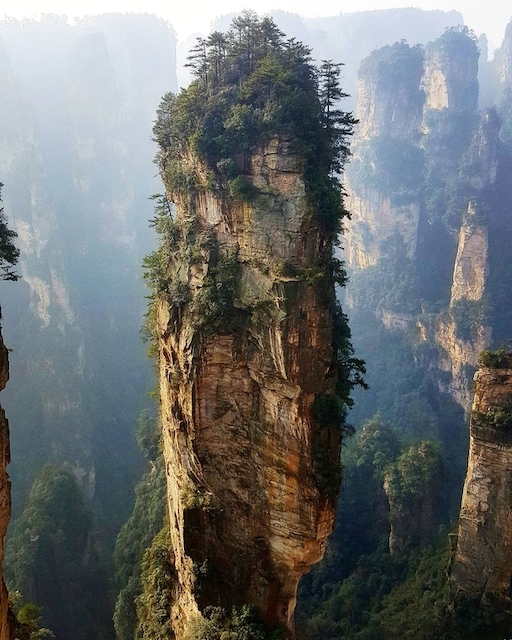
\includegraphics[width=\tmpwidth]{figures/supp_uncropgpt/2_input.jpg} &
 \raisebox{0.85\tmpwidth }{\rotatebox[origin=l]{90}{VQGAN\cite{Esser21vqgan}}} & 
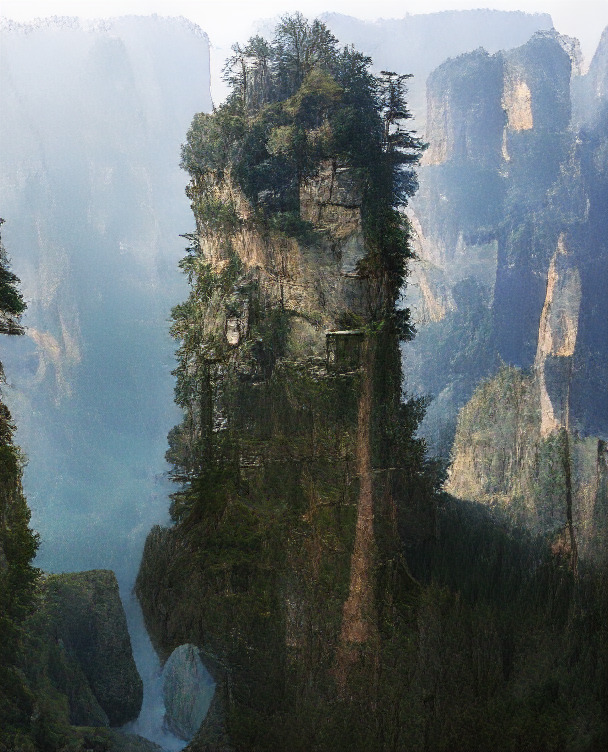
\includegraphics[width=\tmpwidth]{figures/supp_uncropgpt/2_taming1.jpg}&
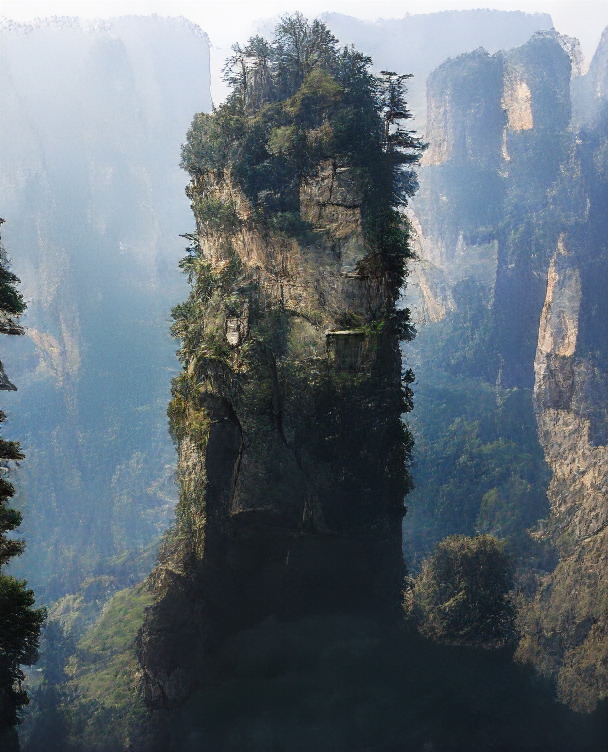
\includegraphics[width=\tmpwidth]{figures/supp_uncropgpt/2_taming2.jpg}&
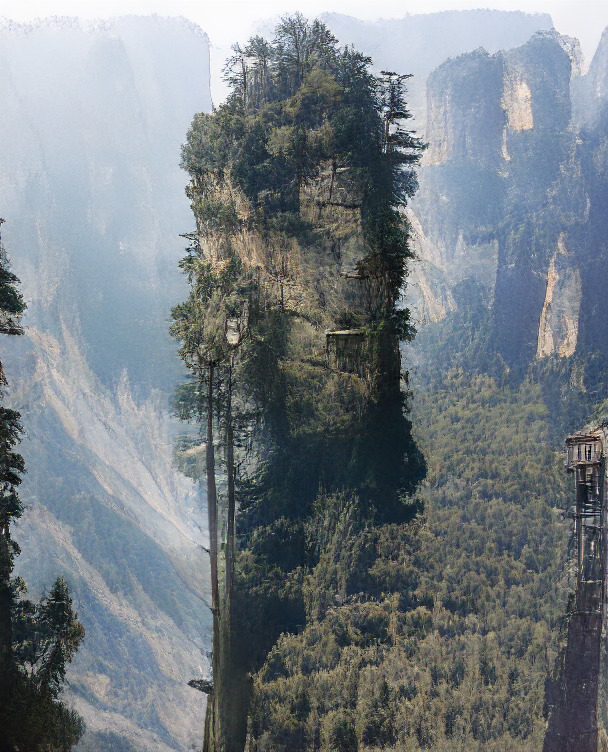
\includegraphics[width=\tmpwidth]{figures/supp_uncropgpt/2_taming3.jpg} &
 \\   
% Groundtruth  & \multicolumn{3}{c}{------ VQGAN\cite{Esser21vqgan}'s Samples ------}  &
% \\

& 
 \raisebox{0.85\tmpwidth }{\rotatebox[origin=l]{90}{\model (Ours)}} & 
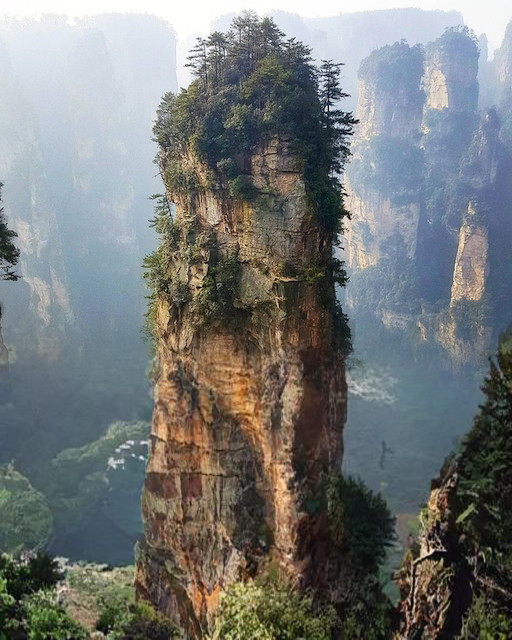
\includegraphics[width=\tmpwidth]{figures/supp_uncropgpt/2_ours4.jpeg}&
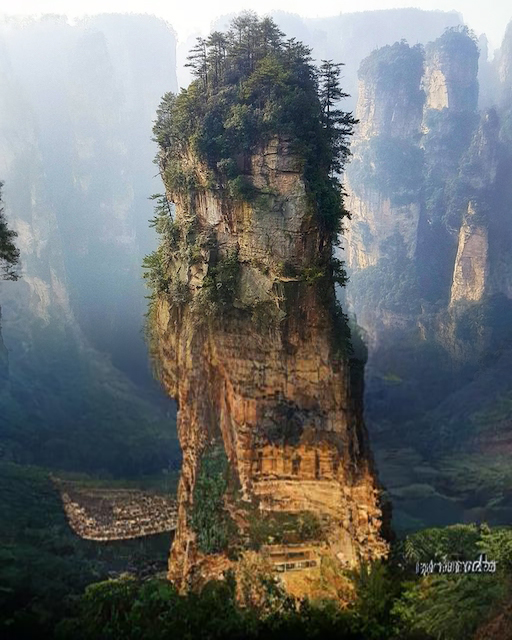
\includegraphics[width=\tmpwidth]{figures/supp_uncropgpt/2_ours11.jpeg}&
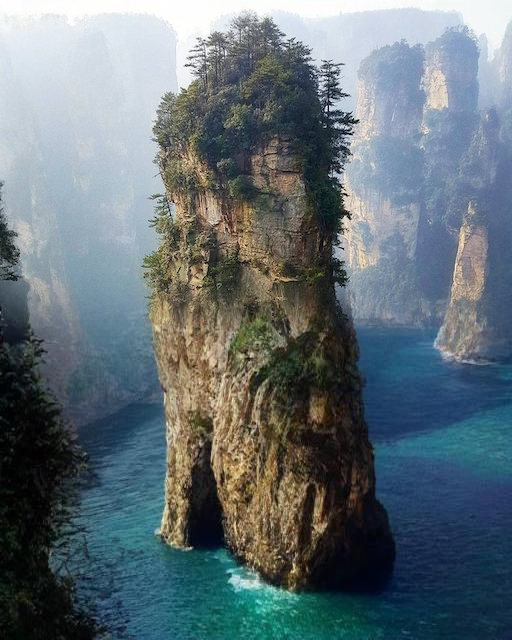
\includegraphics[width=\tmpwidth]{figures/supp_uncropgpt/2_ours19.jpeg} &
&
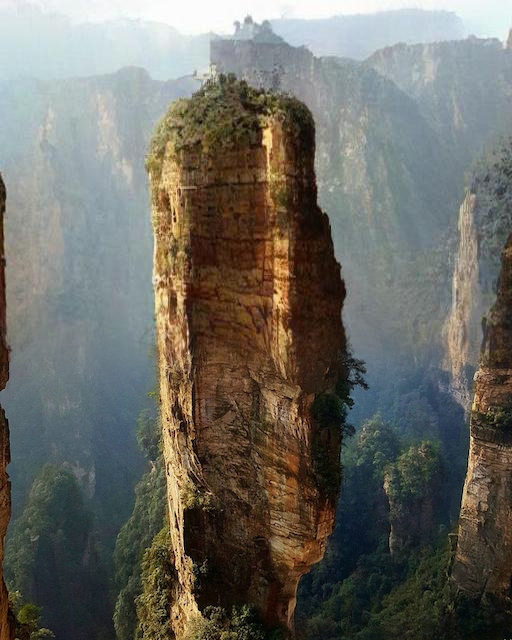
\includegraphics[width=\tmpwidth]{figures/supp_uncropgpt/2_top_ours3.jpeg}&
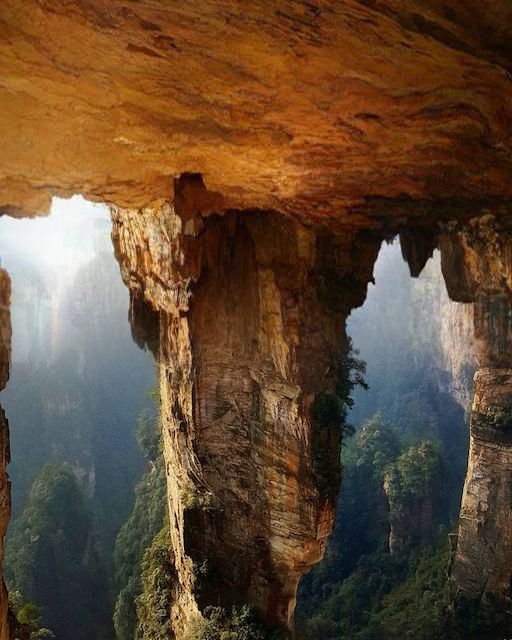
\includegraphics[width=\tmpwidth]{figures/supp_uncropgpt/2_top_ours2.jpeg}&
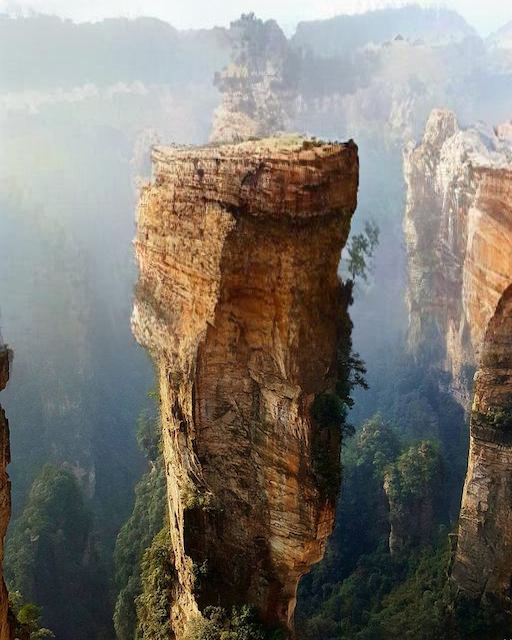
\includegraphics[width=\tmpwidth]{figures/supp_uncropgpt/2_top_ours5.jpeg}
 \\
% &\multicolumn{3}{c}{--- MaskGIT's Samples (Outpainting Bottom Half) ---} &\multicolumn{3}{c}{--- MaskGIT's Samples (Outpainting Top Half) ---}  
% \\ 
       
    \end{tabular}
    \caption{Outpainting comparisons with the pixel-based approach ImageGPT\cite{chen2020imagegpt} and the transformer-based approach VQGAN\cite{Esser21vqgan}.
    }
    % \vspace{-6mm}
    \label{fig:supp_uncropgpt-2}
\end{figure*}





\suppsection{Image Inpainting and Outpainting Comparisons with SOTA GAN-based Approaches}
\label{sec:supp_inpainting_and_outpainting_comparison_with_gans}

In this section, we show more qualitative comparisons with state-of-the-art GAN-based image completion methods in Figure~\ref{fig:supp_inpainting} and Figure~\ref{fig:supp_uncrop_comparison_right}. Quantitative results have been discussed in \ref{ssec:inpainting}. 

We find that compared to prior GAN-based methods, \model demonstrates a stronger capability of completing structures coherently, and its samples contain fewer artifacts. In Figure~\ref{fig:supp_uncrop_comparison_right}, \model completes the bridge in row two and the building in the second to last row, which all GAN methods struggle to do in comparison. 

\renewcommand{\tmpwidth}{27mm}
\setlength{\tabcolsep}{1pt}

\begin{figure*}[!ht]
    \centering
    \begin{tabular}{cccccc}

    Input & DeepFillv2\cite{yu2019free}  & HiFill\cite{yi2020contextual}  & CoModGAN\cite{zhao2021comodgan} & \textbf{\model (Ours)} & Groundtruth \\   
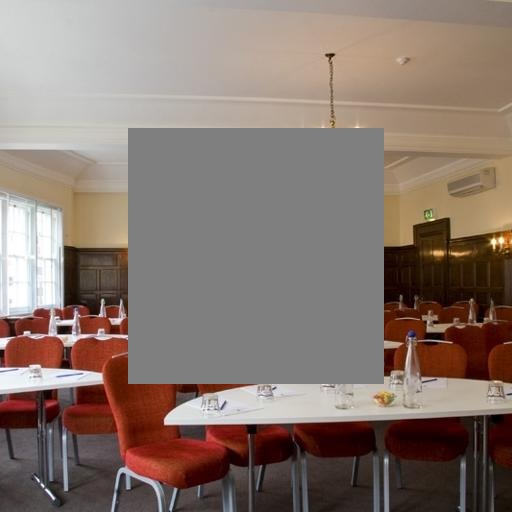
\includegraphics[width=\tmpwidth]{figures/inpaint/000248_input.jpeg}&
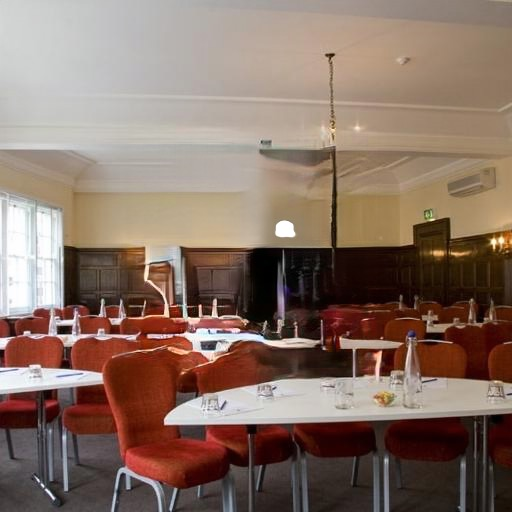
\includegraphics[width=\tmpwidth]{figures/inpaint/000248_deepfillv2.jpeg}&
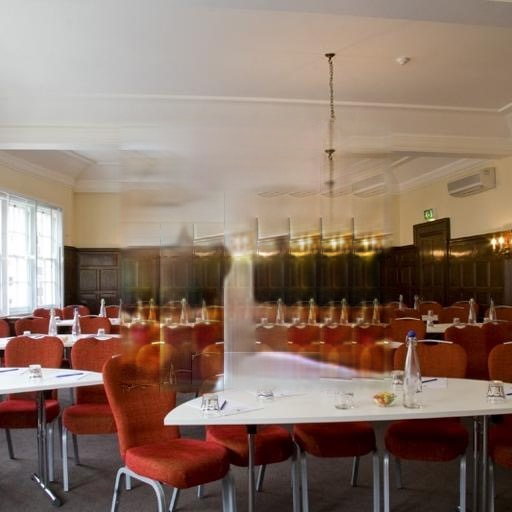
\includegraphics[width=\tmpwidth]{figures/inpaint/000248_hifill.jpeg}&
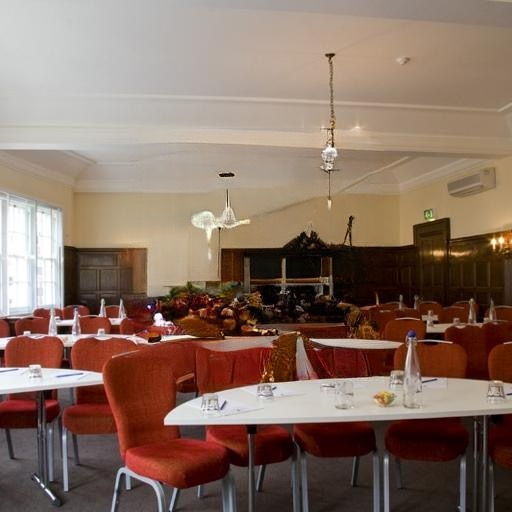
\includegraphics[width=\tmpwidth]{figures/inpaint/000248_comodgan.jpeg}&
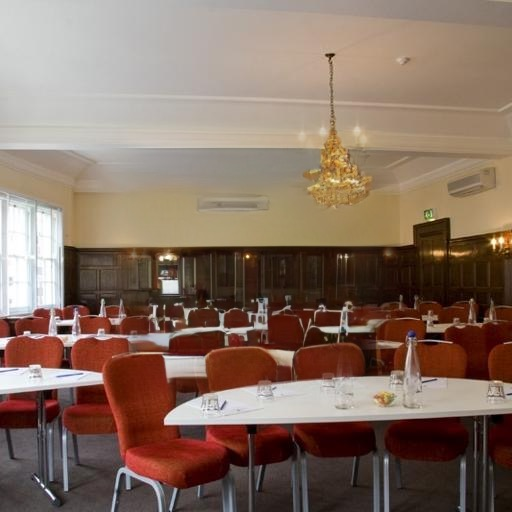
\includegraphics[width=\tmpwidth]{figures/inpaint/000248_ours.jpeg}&
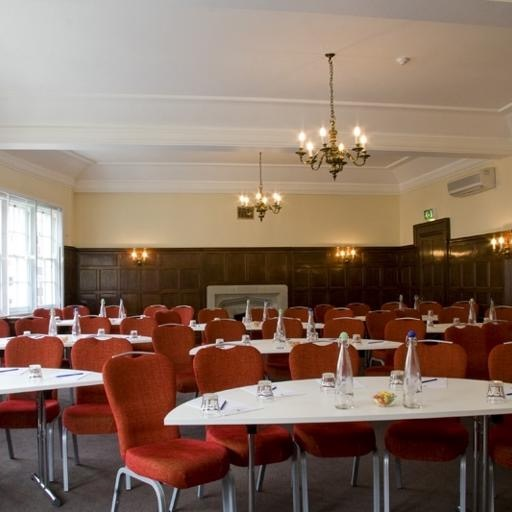
\includegraphics[width=\tmpwidth]{figures/inpaint/000248_gt.jpeg}
\\


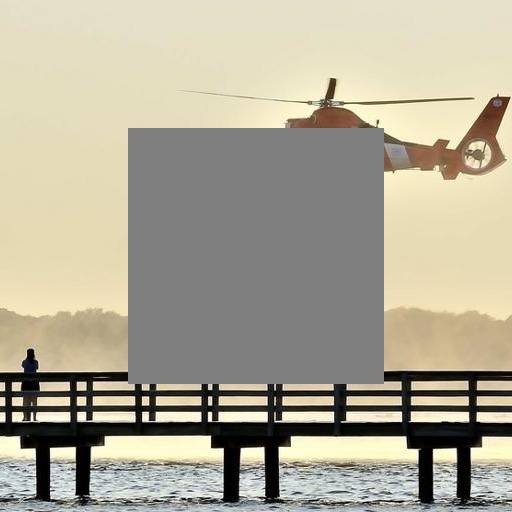
\includegraphics[width=\tmpwidth]{figures/inpaint/000213_input.jpeg}&
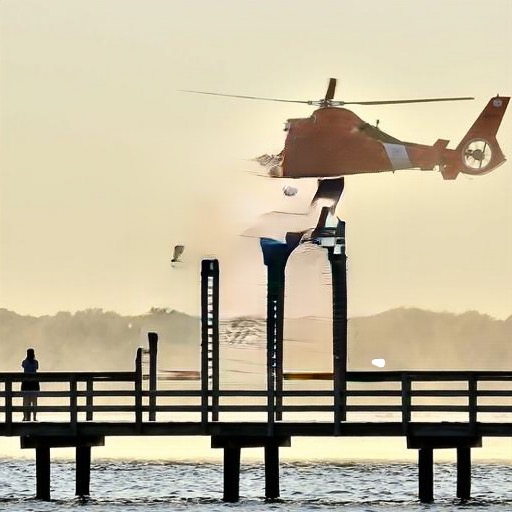
\includegraphics[width=\tmpwidth]{figures/inpaint/000213_deepfillv2.jpeg}&
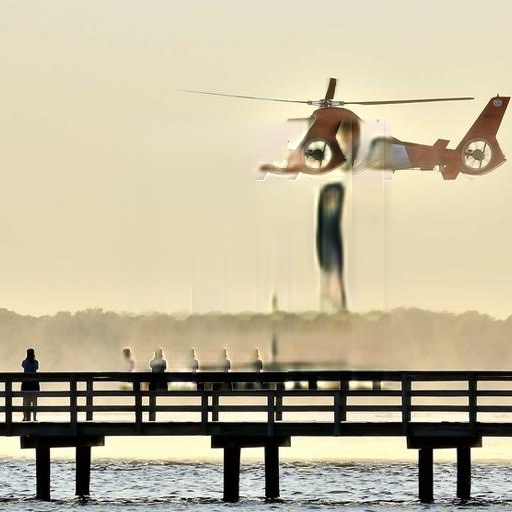
\includegraphics[width=\tmpwidth]{figures/inpaint/000213_hifill.jpeg}&
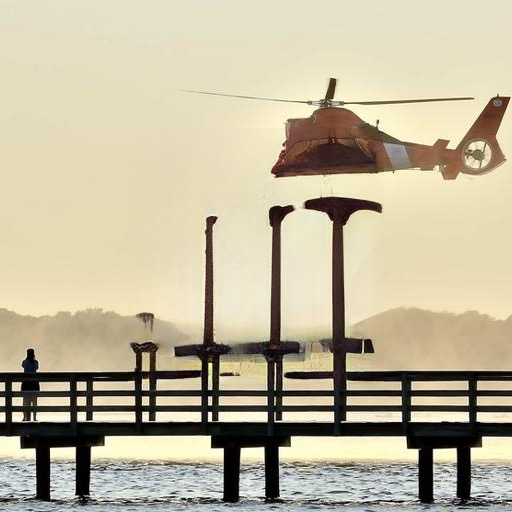
\includegraphics[width=\tmpwidth]{figures/inpaint/000213_comodgan.jpeg}&
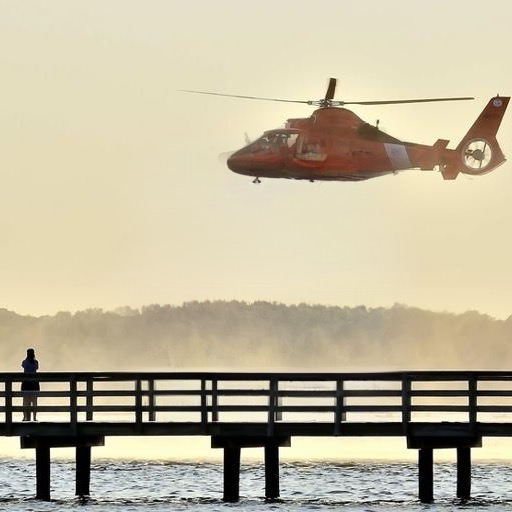
\includegraphics[width=\tmpwidth]{figures/inpaint/000213_ours.jpeg}&
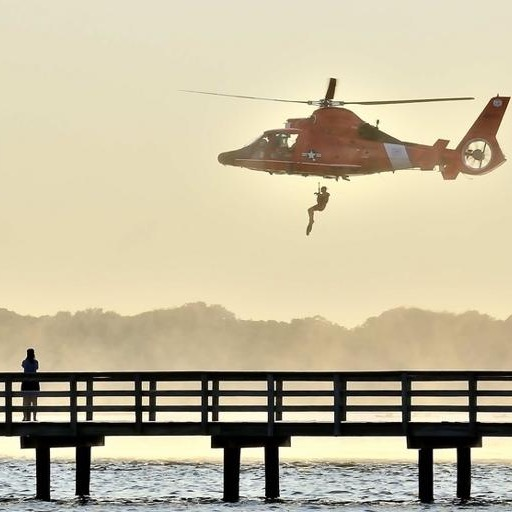
\includegraphics[width=\tmpwidth]{figures/inpaint/000213_gt.jpeg}
\\

% 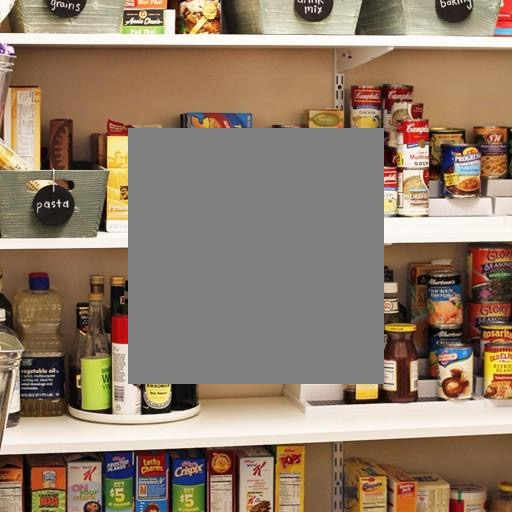
\includegraphics[width=\tmpwidth]{figures/inpaint/000990_input.jpeg}&
% 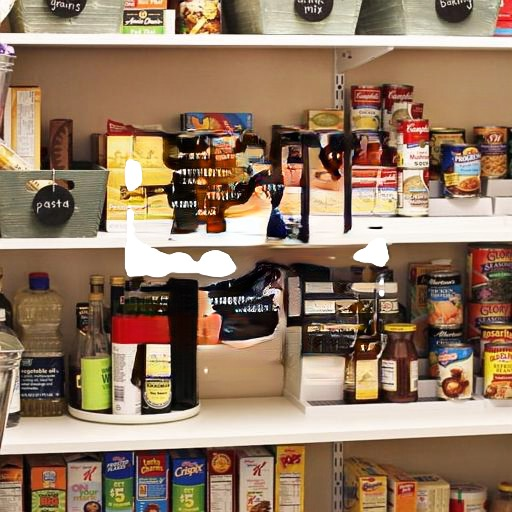
\includegraphics[width=\tmpwidth]{figures/inpaint/000990_deepfillv2.jpeg}&
% 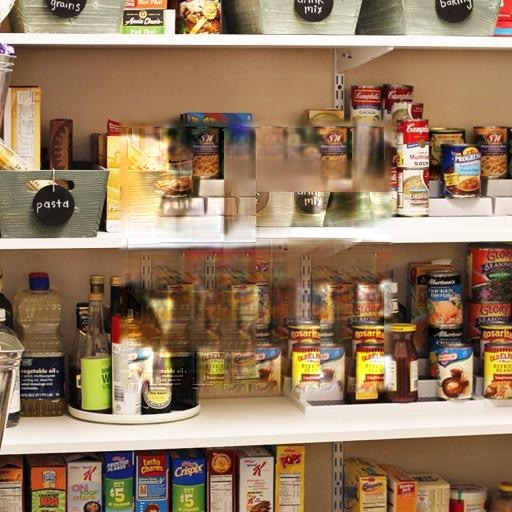
\includegraphics[width=\tmpwidth]{figures/inpaint/000990_hifill.jpeg}&
% 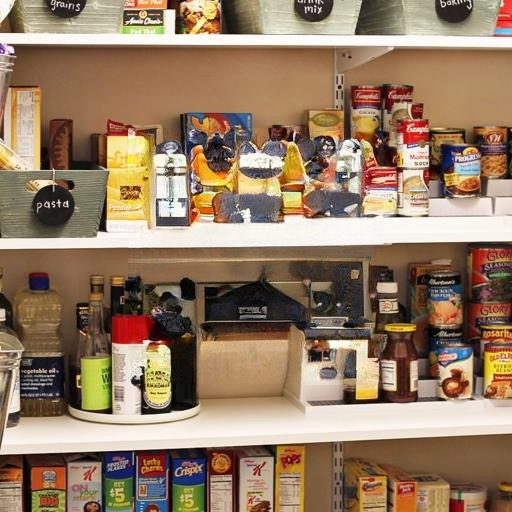
\includegraphics[width=\tmpwidth]{figures/inpaint/000990_comodgan.jpeg}&
% \includegraphics[width=\tmpwidth]{figures/inpaint/000990_ours.jpeg}&
% 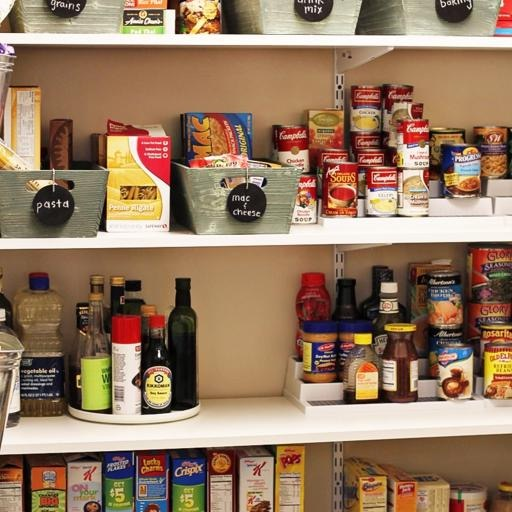
\includegraphics[width=\tmpwidth]{figures/inpaint/000990_gt.jpeg}
% \\

% 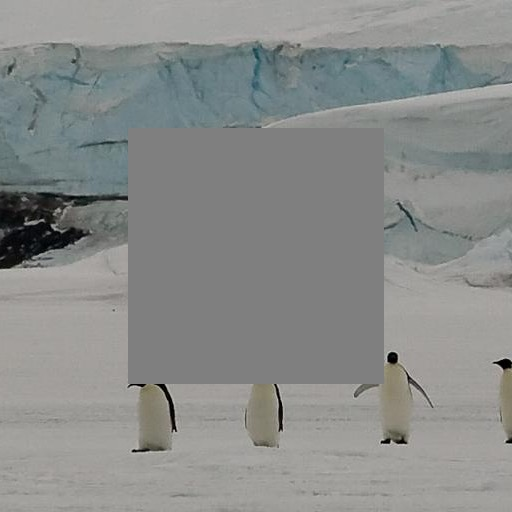
\includegraphics[width=\tmpwidth]{figures/inpaint/000158_input.jpeg}&
% 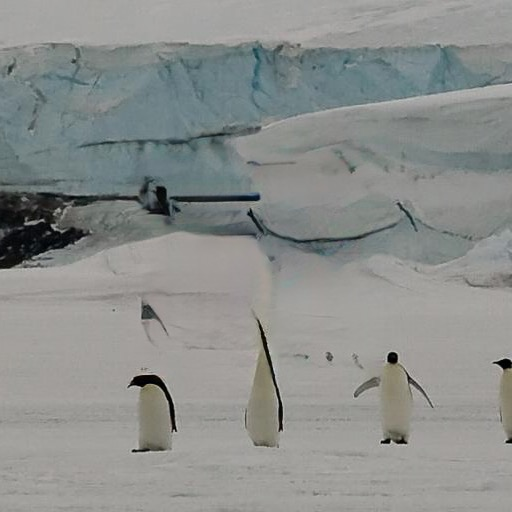
\includegraphics[width=\tmpwidth]{figures/inpaint/000158_deepfillv2.jpeg}&
% 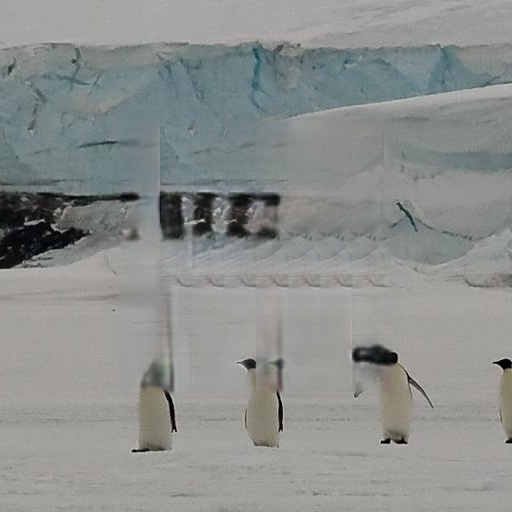
\includegraphics[width=\tmpwidth]{figures/inpaint/000158_hifill.jpeg}&
% 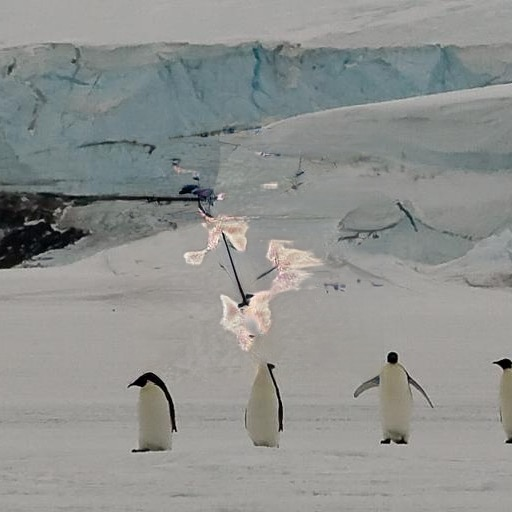
\includegraphics[width=\tmpwidth]{figures/inpaint/000158_comodgan.jpeg}&
% 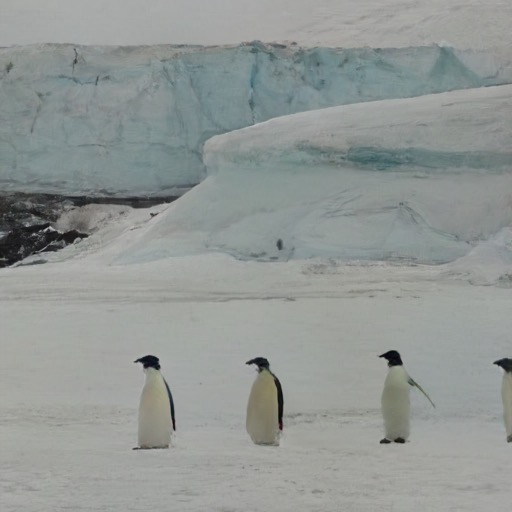
\includegraphics[width=\tmpwidth]{figures/inpaint/000158_ours.jpeg}&
% \includegraphics[width=\tmpwidth]{figures/inpaint/000158_gt.jpeg}
% \\


% \includegraphics[width=\tmpwidth]{figures/inpaint/000966_input.jpeg}&
% \includegraphics[width=\tmpwidth]{figures/inpaint/000966_deepfillv2.jpeg}&
% \includegraphics[width=\tmpwidth]{figures/inpaint/000966_hifill.jpeg}&
% \includegraphics[width=\tmpwidth]{figures/inpaint/000966_comodgan.jpeg}&
% \includegraphics[width=\tmpwidth]{figures/inpaint/000966_ours.jpeg}&
% \includegraphics[width=\tmpwidth]{figures/inpaint/000966_gt.jpeg}
% \\


\includegraphics[width=\tmpwidth]{figures/inpaint/000006_input.jpeg}&
\includegraphics[width=\tmpwidth]{figures/inpaint/000006_deepfillv2.jpeg}&
\includegraphics[width=\tmpwidth]{figures/inpaint/000006_hifill.jpeg}&
\includegraphics[width=\tmpwidth]{figures/inpaint/000006_comodgan.jpeg}&
\includegraphics[width=\tmpwidth]{figures/inpaint/000006_ours.jpeg}&
\includegraphics[width=\tmpwidth]{figures/inpaint/000006_gt.jpeg}
\\

\includegraphics[width=\tmpwidth]{figures/inpaint/000292_input.jpeg}&
\includegraphics[width=\tmpwidth]{figures/inpaint/000292_deepfillv2.jpeg}&
\includegraphics[width=\tmpwidth]{figures/inpaint/000292_hifill.jpeg}&
\includegraphics[width=\tmpwidth]{figures/inpaint/000292_comodgan.jpeg}&
\includegraphics[width=\tmpwidth]{figures/inpaint/000292_ours.jpeg}&
\includegraphics[width=\tmpwidth]{figures/inpaint/000292_gt.jpeg}
\\

\includegraphics[width=\tmpwidth]{figures/inpaint/000285_input.jpeg}&
\includegraphics[width=\tmpwidth]{figures/inpaint/000285_deepfillv2.jpeg}&
\includegraphics[width=\tmpwidth]{figures/inpaint/000285_hifill.jpeg}&
\includegraphics[width=\tmpwidth]{figures/inpaint/000285_comodgan.jpeg}&
\includegraphics[width=\tmpwidth]{figures/inpaint/000285_ours.jpeg}&
\includegraphics[width=\tmpwidth]{figures/inpaint/000285_gt.jpeg}
\\

% \includegraphics[width=\tmpwidth]{figures/inpaint/000060_input.jpeg}&
% \includegraphics[width=\tmpwidth]{figures/inpaint/000060_deepfillv2.jpeg}&
% \includegraphics[width=\tmpwidth]{figures/inpaint/000060_hifill.jpeg}&
% &
% \includegraphics[width=\tmpwidth]{figures/inpaint/000060_ours.jpeg}&
% \includegraphics[width=\tmpwidth]{figures/inpaint/000060_gt.jpeg}
% \\

\includegraphics[width=\tmpwidth]{figures/inpaint/000235_input.jpeg}&
\includegraphics[width=\tmpwidth]{figures/inpaint/000235_deepfillv2.jpeg}&
\includegraphics[width=\tmpwidth]{figures/inpaint/000235_hifill.jpeg}&
\includegraphics[width=\tmpwidth]{figures/inpaint/000235_comodgan.jpeg}&
\includegraphics[width=\tmpwidth]{figures/inpaint/000235_ours.jpeg}&
\includegraphics[width=\tmpwidth]{figures/inpaint/000235_gt.jpeg}
\\

\includegraphics[width=\tmpwidth]{figures/inpaint/000103_input.jpeg}&
\includegraphics[width=\tmpwidth]{figures/inpaint/000103_deepfillv2.jpeg}&
\includegraphics[width=\tmpwidth]{figures/inpaint/000103_hifill.jpeg}&
\includegraphics[width=\tmpwidth]{figures/inpaint/000103_comodgan.jpeg}&
\includegraphics[width=\tmpwidth]{figures/inpaint/000103_ours.jpeg}&
\includegraphics[width=\tmpwidth]{figures/inpaint/000103_gt.jpeg}
\\
    \end{tabular}
    \caption{\textbf{More visual comparisons on image inpainting} on Places2\cite{zhou2017places} with state-of-the-art GAN methods.}

    \label{fig:supp_inpainting}
\end{figure*}



In addition, we compare with CoModGAN on image completion tasks with large masking ratios, \ie conditioning on the center 50$\%\times$50\% and the center 31.25\%$\times$31.25\% respectively, which are challenging cases for traditional GANs. Examples are shown in Figure~\ref{fig:supp_uncrop_comparison}.

\setlength{\tabcolsep}{2pt}
\begin{figure*}[!ht]
    \centering
    \begin{tabular}{cccccc}
        Input & Boundless\cite{teterwak2019boundless} & InfinityGAN\cite{lin2021infinitygan}\footnotesize{\ding{83}} & CoModGAN & \textbf{\model  (Ours)} & Groundtruth \\

    \includegraphics[width=\tmpwidth]{figures/uncrop/5650_005_input.jpeg}&
    \includegraphics[width=\tmpwidth]{figures/uncrop/5650_005_3297_boundless.jpeg}&
    \includegraphics[width=\tmpwidth]{figures/uncrop/5650_005_003297_inf.jpeg}  &
    \includegraphics[width=\tmpwidth]{figures/uncrop/5650_005_comodgan_outpaint_right.jpeg}  &
    \includegraphics[width=\tmpwidth]{figures/uncrop/5650_005_output7.jpeg}&
     \includegraphics[width=\tmpwidth]{figures/uncrop/5650_005_gt.jpeg}

    \\
    \includegraphics[width=\tmpwidth]{figures/uncrop/3101_input.jpeg}&
    \includegraphics[width=\tmpwidth]{figures/uncrop/3101_boundless.jpeg}&
    \includegraphics[width=\tmpwidth]{figures/uncrop/3101_inf.jpeg}&
    \includegraphics[width=\tmpwidth]{figures/uncrop/3101_comodgan_outpaint_right.jpeg}&  
    \includegraphics[width=\tmpwidth]{figures/uncrop/3101_ours.jpeg} &
    % \includegraphics[width=\tmpwidth]{figures/uncrop/3101_output2.jpeg} &
    % \includegraphics[width=\tmpwidth]{figures/uncrop/3101_output4.jpeg} &
    \includegraphics[width=\tmpwidth]{figures/uncrop/3101_gt.jpeg} 
    \\
    \includegraphics[width=\tmpwidth]{figures/uncrop/5604_input.jpeg}&
    \includegraphics[width=\tmpwidth]{figures/uncrop/5604_boundless.jpeg}&
    \includegraphics[width=\tmpwidth]{figures/uncrop/5604_inf.jpeg} &
    \includegraphics[width=\tmpwidth]{figures/uncrop/005604_comodgan_outpaint_right.jpeg} 
    & 
     \includegraphics[width=\tmpwidth]{figures/uncrop/5604_output3.jpeg}&
     \includegraphics[width=\tmpwidth]{figures/uncrop/005604_gt.jpeg}

    \\
   

    %  \includegraphics[width=\tmpwidth]{figures/uncrop/3145_input.jpeg}&
    % \includegraphics[width=\tmpwidth]{figures/uncrop/3145_boundless.jpeg}&
    % \includegraphics[width=\tmpwidth]{figures/uncrop/3145_inf.jpeg}&
    % &
    % \includegraphics[width=\tmpwidth]{figures/uncrop/3145_output7.jpeg}&
    % % \includegraphics[width=\tmpwidth]{figures/uncrop/3145_output1.jpeg}&
    % %\includegraphics[width=\tmpwidth]{figures/uncrop/3145_output2.jpeg}&
    % % \includegraphics[width=\tmpwidth]{figures/uncrop/3145_output6.jpeg}&
    % \includegraphics[width=\tmpwidth]{figures/uncrop/3145_gt.jpeg}
    % \\
   
    
    \end{tabular}
%    \vspace{-3mm}
   % \vspace{-4mm}
    \vspace{-2mm}   
    \caption{\textbf{图像外推的更多视觉比较。}与最先进的 GAN 方法的比较。\ding{83} 样本由作者慷慨提供。
    }
    \label{fig:supp_uncrop_comparison_right}
    \vspace{-8mm}
\end{figure*}    


\begin{figure*}[!ht]
\centering
\begin{tabular}{cccccc}
Input & CoModGAN & \model  (Ours) & Input & CoModGAN & \model  (Ours) \\
\includegraphics[width=\tmpwidth]{figures/uncrop/007658_000_input.jpeg}&
\includegraphics[width=\tmpwidth]{figures/uncrop/007658_000_comodgan_outpaint_center.jpeg}&
\includegraphics[width=\tmpwidth]{figures/uncrop/007658_000_output_02.jpeg}&
\includegraphics[width=\tmpwidth]{figures/uncrop/007658_input_outpaint_center_extreme_larger.jpeg}&

\includegraphics[width=\tmpwidth]{figures/uncrop/007658_000_comodgan_outpaint_center_extreme_larger.jpeg}&

\includegraphics[width=\tmpwidth]{figures/uncrop/007658_024.jpeg} 
\\

\includegraphics[width=\tmpwidth]{figures/uncrop/002046_input.jpeg}&
\includegraphics[width=\tmpwidth]{figures/uncrop/002046_comodgan_outpaint_center.jpeg}&
\includegraphics[width=\tmpwidth]{figures/uncrop/002046_ours_5.jpeg}&
\includegraphics[width=\tmpwidth]{figures/uncrop/002046_input_extreme_larger.jpeg} &
\includegraphics[width=\tmpwidth]{figures/uncrop/002046_comodgan_outpaint_center_extreme_larger.jpeg}&
\includegraphics[width=\tmpwidth]{figures/uncrop/002046_104.jpeg}\\

\includegraphics[width=\tmpwidth]{figures/uncrop/007673_000_input.jpeg} &
\includegraphics[width=\tmpwidth]{figures/uncrop/007673_000_comodgan_outpaint_center.jpeg}&
\includegraphics[width=\tmpwidth]{figures/uncrop/007673_000_output_03.jpeg}&
\includegraphics[width=\tmpwidth]{figures/uncrop/007673_input_outpaint_center_extreme_larger.jpeg}&
\includegraphics[width=\tmpwidth]{figures/uncrop/007673_000_comodgan_outpaint_center_extreme_larger.jpeg}&
\includegraphics[width=\tmpwidth]{figures/uncrop/002046_051.jpeg} \\


\end{tabular}
\vspace{-3mm}
\caption{在大外推掩码上与 CoModGAN\cite{zhao2021comodgan} 的外推视觉比较。}
% \vspace{-4mm}
\label{fig:supp_uncrop_comparison}
\end{figure*}   

\suppsection{Limitations and Failure Cases}
\label{sec:supp_limitations}

In Figure~\ref{fig:supp_failure}, we show several limitations and failure cases of our approach. (A) and (B) are examples of semantic and color shifts in \model's outpainting results. Due to its limited attention size, \model may "forget" the synthesized semantics or color from one end when it's outpainting the other end. (C) and (D) show cases where our approach may sometimes ignore or modify objects on the boundary when applied to outpainting and inpainting. (E) showcases \model's failure mode in which it causes oversmoothing or creates undesired artifacts on complex structures such as human faces, text and symmetric objects. The improvement for these circumstances remains future work. 

\renewcommand{\tmpwidth}{15mm}
\newcommand{\tmpheight}{30mm}
\setlength{\tabcolsep}{4pt}
\begin{figure*}[!ht]
    \centering
    %\renewcommand{\arraystretch}{2}
    \begin{tabular}{m{10mm}c c}

% (A) & \parbox[c]{\tmpwidth}{\includegraphics[ height=\tmpheight]{figures/supp_failure/chelsea-gates-0653_wY0nRc-unsplash.jpg_input.jpeg}} &
% \parbox[c]{9\tmpwidth}{\includegraphics[ height=\tmpheight]{figures/supp_failure/chelsea-gates-0653_wY0nRc-unsplash.jpg_output0006_1.jpeg}}
% \\ 

& Input & \parbox[c]{8\tmpwidth}{Our Outpainting Samples}  \\

~~~~~(A) & \parbox[c]{\tmpwidth}{\includegraphics[ height=\tmpheight]{figures/supp_failure/christoph-schulz-7tb-b37yHx4-unsplash.jpg}}  & 
\parbox[c]{9\tmpwidth}{\includegraphics[ height=\tmpheight]{figures/supp_failure/christoph-schulz-7tb-b37yHx4-unsplash.jpg_output0006_1.jpeg}}
 \\ 
 
 
%  & Input & \parbox[c]{8\tmpwidth}{Our outpainting samples} \\ 
 
~~~~~(B) & \parbox[c]{\tmpwidth}{\includegraphics[ height=\tmpheight]{figures/panorama/janosch-diggelmann-qXzNdOfGnbw-unsplash.jpg}}  & 
\parbox[c]{9\tmpwidth}{\includegraphics[ height=\tmpheight]{figures/supp_failure/janosch-diggelmann-qXzNdOfGnbw-unsplash.jpg_input.jpeg}}
 \\ 
%  (C) & \parbox[c]{\tmpwidth}{\includegraphics[ height=\tmpheight]{figures/panorama/damiano-baschiera-hFXZ5cNfkOk-unsplash.jpg}}  & 
% \parbox[c]{9\tmpwidth}{\includegraphics[ height=\tmpheight]{figures/supp_failure/damiano-baschiera-hFXZ5cNfkOk-unsplash.jpg_output0001_1.jpeg}}
%  \\ 
 \end{tabular}
 \setlength{\tabcolsep}{1pt}
 \begin{tabular}{m{7mm}c c c c c }
    & Input & \multicolumn{3}{c}{------ Our Outpainting Samples ------} & Groundtruth
    \\
 (C) & 
     \parbox[c]{\tmpheight}{\includegraphics[height=\tmpheight]{figures/uncrop/2982_input.jpeg}}&
    % \parbox[c]{\tmpheight}{\includegraphics[height=\tmpheight]{figures/uncrop/2982_boundless.jpeg}}&
    % \parbox[c]{\tmpheight}{\includegraphics[height=\tmpheight]{figures/uncrop/2982_inf.jpeg}}&
    \parbox[c]{\tmpheight}{\includegraphics[height=\tmpheight]{figures/uncrop/2982_output5.jpeg}} &
    % \parbox[c]{\tmpheight}{\includegraphics[height=\tmpheight]{figures/uncrop/2982_output0.jpeg}} &
    \parbox[c]{\tmpheight}{\includegraphics[height=\tmpheight]{figures/uncrop/2982_output9.jpeg}} &
    \parbox[c]{\tmpheight}{\includegraphics[height=\tmpheight]{figures/uncrop/2982_output3.jpeg}} &
    % \parbox[c]{\tmpheight}{\includegraphics[height=\tmpheight]{figures/uncrop/2982_output10.jpeg}} &
   \parbox[c]{\tmpheight}{ \includegraphics[height=\tmpheight]{figures/uncrop/2982_gt.jpeg}}
  \\
   & Input & \multicolumn{3}{c}{------Our Inpainting Samples ------} & Groundtruth 
   \\
  (D) & 
     \parbox[c]{\tmpheight}{\includegraphics[height=\tmpheight]{figures/uncrop/2142_003_input.jpeg}}&
    % \parbox[c]{\tmpheight}{\includegraphics[height=\tmpheight]{figures/uncrop/2982_boundless.jpeg}}&
    % \parbox[c]{\tmpheight}{\includegraphics[height=\tmpheight]{figures/uncrop/2982_inf.jpeg}}&
    \parbox[c]{\tmpheight}{\includegraphics[height=\tmpheight]{figures/uncrop/2142_003_output6.jpeg}} &
    % \parbox[c]{\tmpheight}{\includegraphics[height=\tmpheight]{figures/uncrop/2982_output0.jpeg}} &
    \parbox[c]{\tmpheight}{\includegraphics[height=\tmpheight]{figures/uncrop/2142_003_output9.jpeg}} &
    \parbox[c]{\tmpheight}{\includegraphics[height=\tmpheight]{figures/uncrop/2142_003_output14.jpeg}} &
    % \parbox[c]{\tmpheight}{\includegraphics[height=\tmpheight]{figures/uncrop/2982_output10.jpeg}} &
   \parbox[c]{\tmpheight}{ \includegraphics[height=\tmpheight]{figures/uncrop/2142_003_gt.jpeg}}
  \\
   & \multicolumn{5}{c}{------Our Class-conditional Samples ------} \\
(E) & \parbox[c]{\tmpheight}{\includegraphics[height=\tmpheight]{figures/supp_failure/000417_0010_output.jpeg}} & 
%  \parbox[c]{\tmpheight}{\includegraphics[height=\tmpheight]{figures/supp_failure/000967_0009_output.jpeg}} & 
\parbox[c]{\tmpheight}{\includegraphics[height=\tmpheight]{figures/supp_failure/000454_0004_output.jpeg}} & 
\parbox[c]{\tmpheight}{\includegraphics[height=\tmpheight]{figures/supp_failure/000918_0031.jpeg}} &
\parbox[c]{\tmpheight}{\includegraphics[height=\tmpheight]{figures/supp_failure/000661_0006.jpeg}} &
\parbox[c]{\tmpheight}{\includegraphics[height=\tmpheight]{figures/supp_failure/000831_0036_output.jpeg}}
  
 \\
   \end{tabular}
    \caption{局限性和失败案例。}
    \vspace{-6mm}
    \label{fig:supp_failure}
\end{figure*}

